% !TeX TS-program = pdflatex

% PREAMBLE BU ECE template for MS thesis and PhD dissertation. Additions from
% https://github.com/scivision/phd-thesis-dissertation/blob/master/thesis.tex

% MAIN LAYOUT
\pdfminorversion=7
\documentclass[12pt,letterpaper]{report}
\usepackage[utf8]{inputenc}
\usepackage[T1]{fontenc}
\usepackage[toc,page]{appendix}
% \usepackage{subfiles}

% BIBLIOGRAPHY/REFERENCES
% \usepackage{biblatex}
% \addbibresource{thesis.bib}
% \addbibresource{ref.bib}
% \usepackage{natbib}
% \usepackage{apalike}
% \bibliographystyle{plain}

% BOSTON UNIVERSITY THESIS/DISSERTATION
\usepackage{bu_ece_thesis}

% FIGURES/GRAPHICS
\usepackage{graphicx}
\usepackage{float}
\graphicspath{ {figures/} {./figures/} {../figures/} }
\DeclareGraphicsExtensions{.jpg,.png,.eps,.pdf}

% CAPTIONS
\usepackage[bf]{caption}
\usepackage{subcaption}
% \usepackage[format=hang,justification=raggedright,singlelinecheck=0,labelsep=period]{caption}
% \usepackage[format=hang,justification=raggedright,singlelinecheck=0,labelsep=period]{subcaption}

% NOMENCLATURE
\usepackage[intoc, english]{nomencl}
\makenomenclature{}
% todo

% MATH and FONTS
\usepackage[intlimits]{amsmath}
\usepackage{amsfonts,amssymb}
\DeclareSymbolFontAlphabet{\mathbb}{AMSb}
\usepackage{fancyhdr}
\usepackage{fancybox}
\usepackage{ifthen}
\usepackage{lscape,afterpage}
\usepackage{xspace}
\usepackage{booktabs}
\usepackage{algorithm,algpseudocode}


% LINKS
\usepackage[unicode=true]{hyperref}
\hypersetup{breaklinks=true,bookmarks=true,pdfborder={0 0 0},colorlinks=false}
% pdfauthor=\author,pdftitle=\title

% FIG/TABLE/EQN REFERENcES
\usepackage{cleveref}
\usepackage{listings}
%==========================================================================%
\newcommand{\figref}[1]{Figure~\ref{#1}}
\newcommand{\chapref}[1]{Chapter~\ref{#1}}
\newcommand{\secref}[1]{Section~\ref{#1}}
\usepackage{enumitem}
\usepackage{pdfpages}

% CODE HIGHLIGHTING
\usepackage[]{minted}
\usemintedstyle{monokai}
\setminted{bgcolor=darkgray,breaklines=true,fontsize=\footnotesize}
\renewcommand\listoflistingscaption{List of source code}

% CHARTS
\usepackage{units}
\usepackage[section]{placeins}
\usepackage{flowchart}

% % PREAMBLE
% BU ECE template for MS thesis and PhD dissertation.
% Additions from https://github.com/scivision/phd-thesis-dissertation/blob/master/thesis.tex

% MAIN LAYOUT
\pdfminorversion=7
\documentclass[12pt,letterpaper]{report}
\usepackage[utf8]{inputenc}
\usepackage{appendix}
\usepackage{subfiles}

% BOSTON UNIVERSITY THESIS/DISSERTATION
\usepackage{bu_ece_thesis}

% FIGURES/GRAPHICS
\usepackage{graphicx,grffile}
\makeatletter
\let\@currsize\normalsize
\dev\maxwidth{\ifdim\Gin@nat@width>\linewidth\linewidth\else\Gin@nat@width\fi}
\dev\maxheight{\ifdim\Gin@nat@width>\textheight\textheight\else\Gin@nat@width\fi}
\makeatother
\setkeys{Gin}{width=\maxwidth,height=\maxheight,keepaspectratio}
\usepackage{float}
\usepackage{rotating}
\usepackage{subfig}
\setcaptionmargin{0.5in}
\usepackage{psfrag}

% CAPTIONS
\usepackage[bf]{caption}
\usepackage{subcaption}
\usepackage{floatrow}

% GRAPHICS PATHS
\graphicspath{ {figures/} {./figures/} {../figures/} }
\DeclareGraphicsExtensions{.jpg,.png,.eps,.pdf}


% MATH and FONTS
\usepackage[intlimits]{amsmath}
\usepackage{amsfonts,amssymb}
\DeclareSymbolFontAlphabet{\mathbb}{AMSb}
% \usepackage[T1]{fontenc}
% \usepackage[intlimits]{mathtools}
% \usepackage{mathrsfs} %enables formal \mathscr
% \usepackage{textcomp} % \textdegree  %gensymb $\degree$


% \usepackage{natbib}
\usepackage{apalike}
\usepackage{fancyhdr}
\usepackage{fancybox}
\usepackage{ifthen}
\usepackage{lscape,afterpage}
\usepackage{xspace}
\usepackage{booktabs}
\usepackage{algorithm,algpseudocode}

% LINKS
\usepackage[unicode=true]{hyperref}
\hypersetup{breaklinks=true,bookmarks=true,pdfborder={0 0 0},colorlinks=false}
% pdfauthor=\author,pdftitle=\title

% FIG/TABLE/EQN REFERENcES
\usepackage{cleveref}
% \usepackage{listings}
% \usepackage[format=hang,justification=raggedright,singlelinecheck=0,labelsep=period]{caption}
% \usepackage[format=hang,justification=raggedright,singlelinecheck=0,labelsep=period]{subcaption}

%==========================================================================%
% customized commands can be placed here
\newcommand{\figref}[1]{Figure~\ref{#1}}
\newcommand{\chapref}[1]{Chapter~\ref{#1}}
\newcommand{\latex}{\LaTeX\xspace}

\usepackage{xargs}
\usepackage[colorinlistoftodos,prependcaption,textsize=small]{todonotes}
\newcommandx{\unsure}[2][1=]{\todo[linecolor=red,backgroundcolor=red!25,bordercolor=red,#1]{#2}}
\newcommandx{\change}[2][1=]{\todo[linecolor=blue,backgroundcolor=blue!25,bordercolor=blue,#1]{#2}}
\newcommandx{\info}[2][1=]{\todo[linecolor=OliveGreen,backgroundcolor=OliveGreen!25,bordercolor=OliveGreen,#1]{#2}}
\newcommandx{\improvement}[2][1=]{\todo[linecolor=Plum,backgroundcolor=Plum!25,bordercolor=Plum,#1]{#2}}
%==========================================================================%

% % % % %
\DeclareMathOperator*{\argmin}{\arg\!\min}
\DeclareMathOperator*{\argmax}{\arg\!\max}

% % % % % % % % % % % % % % % % % % % % % % % % % % % %
\usepackage{units} %necessary for \nicefrac
\usepackage{epigraph}
\usepackage[section]{placeins}
\usepackage{tikz}

\usepackage{flowchart}

%\usepackage[clean]{svg} doesn't work in linux or windows for this style...
% % % % % % % % % %
\usepackage{marginnote}
% % % % % % % % % % % % % % % %
\usepackage{harpoon} %my favorite vector
\newcommand*{\vect}[1]{\overrightharp{\ensuremath{#1}}}
% % % % % % % % % % % % % % %
\usetikzlibrary{shapes.geometric,arrows}
%
\tikzstyle{startstop} = [rectangle, rounded corners, text centered, draw=black, fill=blue!10]
\tikzstyle{process} = [rectangle, minimum width=2cm,  text centered, draw=black, fill=orange!10]
\tikzstyle{decision} = [diamond, aspect=3, minimum width=3cm, minimum height=1cm, text centered, draw=black, fill=red!10]
% define arrow style
\tikzstyle{compute} = [rectangle, minimum width=2cm, minimum height=1cm, text centered, draw=black, fill=green!10]
\tikzstyle{estimate} = [rectangle, rounded corners, minimum width=2cm, minimum height=1cm, text centered, draw=black, fill=yellow!10]
\tikzstyle{arrow} = [thick,->,>=stealth]
% % % % % % % % % % %
%\usetikzlibrary{matrix,positioning} % math matrices
% % % % % % % % % % % % % % %
\usepackage{enumitem}
\usepackage{pdfpages}
% % % % % % % % % % %


\begin{document}

%%%%%%%%%%%%%%%%%%%%%%%%%%%%%%%%%%%%%%%%%%%%%%%%%%%%%%%%%%%%%%%%
% INFO
%%%%%%%%%%%%%%%%%%%%%%%%%%%%%%%%%%%%%%%%%%%%%%%%%%%%%%%%%%%%%%%%

\title{
    Tools for interfacing, extracting, and analysing neural signals using wide-field fluorescence imaging and optogenetics in awake behaving mice}

\author{Mark E. Bucklin}

\degree=2

\prevdegrees{B.S., Columbia University, 2009\\ M.S., Boston University, 2016}

\department{Department of Biomedical Engineering}

\defenseyear{2019} \degreeyear{2019}

\reader{First}{Xue Han, Ph.D.
}{% the title in with the name.% because it will overflow to a new page. You may try to put part of% Warning: If you have more than five readers you are out of luck,% or you will be asked to reprint and get new signatures.%   Professor, Department of Electrical and Computer Engineering"% or similar, but it MUST NOT be:%   "Professor of Electrical and Computer Engineering",% then name, and title. IMPORTANT: The title should be:% For each reader, specify appropriate label {First, Second, Third},% January of year X+1% will be in the fall of year X, and your graduation will be in% will be the same, except for January graduation, when your defense% the year the dissertation is written up and defended. Often, these% Degree year is the year the diploma is expected, and defense year is%   3 = Master of Science thesis and Doctor of Philisophy dissertation.%   2 = Doctor of Philisophy dissertation.%   1 = Master of Science thesis,% Type of document prepared for this degree:
    Associate Professor of Biomedical Engineering} \reader{Second}{David Boas, Ph.D.
}{
    Professor of Biomedical Engineering} \reader{Third}{Ian Davison, Ph.D.
}{
    Assistant Professor of Biology} \reader{Fourth}{Jerome C.
    Mertz, Ph.D.
}{
    Professor of Department of Biomedical Engineering} \reader{Fifth}{Kamal Sen, Ph.D.
}{
    Associate Professor of Biomedical Engineering}

\numadvisors=1 \majorprof{Xue Han, Ph.D.
}{{Associate Professor of Biomedical Engineering}}% (advisors) can be defined. % specified again for the abstract page. Up to 4 Major Professors% The Major Professor is the same as the first reader, but must be
%\majorprofb{First M. Last, PhD}{{Professor of Computer Science}}
%\majorprofc{First M. Last, PhD}{{Professor of Astronomy}}
%\majorprofd{First M. Last, PhD}{{Professor of Biomedical Engineering}}


% Order
% - title
% - copyright
% - approval
% - dedication
% - acknowledgements
% - abstract
% - preface
% - table-of-contents
% - list-of-tables
% - list-of-figures
% - list-of-source-code
% - list-of-abbreviations
% - glossary

% - chapter1
% - chapter2
% - chapter3
% - chapter4

% - appendices
% - bibliography
% - curriculum-vita

%%%%%%%%%%%%%%%%%%%%%%%%%%%%%%%%%%%%%%%%%%%%%%%%%%%%%%%%%%%%%%%%
% PRE (preliminary pages in before body)
%%%%%%%%%%%%%%%%%%%%%%%%%%%%%%%%%%%%%%%%%%%%%%%%%%%%%%%%%%%%%%%%

% TITLE
\maketitle
\clearpage{}

% COPYRIGHT
\copyrightpage
\clearpage{}

% APPROVAL-PAGE
\approvalpage
\clearpage{}

% DEDICATION
\newpage
\begin{center}
\centerline{for pickle}
\end{center}

\clearpage{}

% ACKNOWLEDGEMENTS
\newpage
\chapter*{Acknowledgements}\label{acknowledgements}

The support and patience I have received from my committee has gone far beyond what should be expected of anyone.
I can't thank you enough.
\begin{itemize}
	\item Xue Han, Ph.D.
	\item David Boas, Ph.D.
    \item Kamal Sen Ph.D.
	\item Jerome Mertz, Ph.D.
	\item Ian Davison, Ph.D.
	\item Vickery Trinkaus-Randall, Ph.D.
	\item Steven Borkan, M.D.
\end{itemize}

\vskip 1in

\clearpage{}

% ABSTRACT
\begin{abstractpage}
% ABSTRACT

Imaging of multiple cells has rapidly multiplied the rate of data acquisition as well as our knowledge of the complex dynamics within the mammalian brain.
The process of data acquisition has been dramatically enhanced with highly affordable, sensitive image sensors enable high-throughput detection of neural activity in intact animals.
Genetically encoded calcium sensors deliver a substantial boost in signal strength and in combination with equally critical advances in the size, speed, and sensitivity of image sensors available in scientific cameras enables high-throughput detection of neural activity in behaving animals using traditional wide-field fluorescence microscopy.
However, the tremendous increase in data flow presents challenges to processing, analysis, and storage of captured video, and prompts a reexamination of traditional routines used to process data in neuroscience and now demand improvements in both our hardware and software applications for processing, analyzing, and storing captured video.
This project demonstrates the ease with which a dependable and affordable wide-field fluorescence imaging system can be assembled and integrated with behavior control and monitoring system such as found in a typical neuroscience laboratory.

An Open-source MATLAB toolbox is employed to efficiently analyze and visualize large imaging data sets in a manner that is both interactive and fully automated.
This software package provides a library of image pre-processing routines optimized for batch-processing of continuous functional fluorescence video, and additionally automates a fast unsupervised ROI detection and signal extraction routine.
Further, an extension of this toolbox that uses GPU programming to process streaming video, enabling the identification, segmentation and extraction of neural activity signals on-line is described in which specific algorithms improve signal specificity and image quality at the singe cell level in a behaving animal.
This  project describes the strategic ingredients for transforming a large bulk flow of raw continuous video into proportionally informative images and knowledge.


%

\end{abstractpage}
\clearpage{}

% PREFACE
\newpage
\chapter*{Preface}\label{preface}

I have structured this document to roughly coincide with a chronological account of 6 years spent in a neuro-oriented biomedical engineering lab.
My role in the lab was centered around exploratory device design and development, mostly targeting application in neuroscience research, with intended users being neuroscientist colleagues.
One of the lab's most remarkable assets is the breadth and diversity of its constituents in terms of their skills and experience, both within and between the engineering/development and the science/medical sides of the lab.
All efforts stood to benefit from the close proximity to skilled colleagues, most notably for the complementary guide and provide roles that assisted the development process of new devices and the experiments they were intended for.

My initial experience in optoelectronic device development was as an undergrad at Columbia University where I was advised by Elizabeth Hillman, and developed a device that combined thermography and near-infrared spectroscopy in a portable and inexpensive device intended to provide early detection of adverse neoplastic changes through at-home daily monitoring, particularly targeting use by patients with high-risk for breast cancer.
I then went to the Das Lab where I developed macroscopic imaging systems used for intrinsic imaging in the visual cortex of awake primates.
As a MD/PhD student, I attempt to maintain a potential to adapt the end-products of each development for clinical applicability.
The story presented here is rather unusual in that success precedes failure.
The volume of tangible presentable results is greatest toward the beginning stages of the work described here.
This unusual inversion is what make this story worth hearing, however.
Thank you for taking the time to read this.
I hope that at least the technical information provided herein, if not the procedural insight, is valuable in your current or future endeavors.

\clearpage{}

% TABLE OF CONTENTS
\tableofcontents
\clearpage{}

% LIST OF TABLES
% \newpage
% \listoftables
% \clearpage{}

% LIST OF FIGURES
\newpage
\listoffigures
\clearpage{}

% LIST OF CODE
\newpage
\listoflistings
\clearpage{}

% LIST OF ABBREVIATIONS
\newpage
\chapter*{List of Abbreviations}\label{list-of-abbreviations}

\begin{center}
    \begin{tabular}{lll}
        \hspace*{2em}    & \hspace*{1in} & \hspace*{4.5in}                        \\
      AAV               & \dotfill      & Adeno-Associated Virus  \\
      ALU               & \dotfill      & Arithmetic Logic Unit \\
      BLAS               & \dotfill      & Basic Linear Algebra Subprograms \\
      CMOS               & \dotfill      & Complementary Metal Oxide Semiconductor  \\
      CUDA               & \dotfill      & Compute Unified Device Architecture \\
      DVS               & \dotfill      & Dynamic Vision Sensor \\
      FFT               & \dotfill      & Finite Fourier Transform  \\
      GCaMP6               & \dotfill      & Green Calmodulin Protein 6 \\
      GECI               & \dotfill      & Genetically Encoded Calcium Indicator  \\
      GFP               & \dotfill      & Green Fluorescent Protein \\
      GPU               & \dotfill      & Graphics Processing Unit  \\
      IFFT               & \dotfill      & Inverse Finite Fourier Transform \\
      LED               & \dotfill      & Light Emitting Diode  \\
      LINPACK               & \dotfill      & Linear Algebra Package  \\
      PCA               & \dotfill      & Principal Component Analysis  \\
      PMI               & \dotfill      & Pointwise Mutual Information  \\
      POS               & \dotfill      & Point of Sale \\
      REPL               & \dotfill      & Read Evaluate Print Loop \\
      ROI               & \dotfill      & Region of Interest  \\
      SIMD               & \dotfill      & Single Instruction Multiple Data \\
      SPMD               & \dotfill      & Single Program Multiple Data \\
      nPMI               & \dotfill      & Normalized Pointwise Mutual Information  \\
      sCMOS               & \dotfill      & Scientific Complementary Metal Oxide Semiconductor \\
    \end{tabular}
\end{center}


\clearpage{}

% \newpage
% \endofpre

%%%%%%%%%%%%%%%%%%%%%%%%%%%%%%%%%%%%%%%%%%%%%%%%%%%%%%%%%%%%%%%%
% CHAPTERS (MAIN BODY OF DOCUMENT)
%%%%%%%%%%%%%%%%%%%%%%%%%%%%%%%%%%%%%%%%%%%%%%%%%%%%%%%%%%%%%%%%

% CHAPTER 1: INTRODUCTION
% \documentclass[../main.tex]{subfiles}
% \begin{document}

\thispagestyle{myheadings}

\chapter{Introduction: Background and Literature Review}
\label{sec:introduction}


\section{Optical Imaging of Neural Activity}\label{sec:optical-imaging-of-neural-activity}

Optical techniques for observing neural activity have recently advanced owing to both an evolution of digital imaging technology, and the development of engineered proteins that act as fluorescent indicators of neural activity.
Image sensors, like those found in scientific-CMOS (sCMOS) cameras are larger, faster, and more sensitive than prior scientific grade cameras.
Meanwhile, the latest generation of Genetically Encoded Calcium Indicators (GECIs), collectively called GCaMP6, report fluctuations in neural activation with extremely high fidelity.
This combination of developments enables neuroscientists to open a wider channel to the brain than previously possible using conventional epifluorescence microscopy techniques that enable simultaneous recording from hundreds to thousands of neurons.
Expanding the fraction of the observable neurons in an interconnected network could improve understanding of neural coding and provide insight into mechanistic properties of neural disease.
Additionally, feeding a large set of neural response information to a machine learning algorithm in a neuro-prosthetic application may provide improved predictive performance even when the exact mechanism of prediction is difficult to discern.
However, several major challenges currently antagonize the potential benefits of these new technologies:

\begin{enumerate}
	\def\labelenumi{\arabic{enumi}.}
	\itemsep1pt\parskip0pt\parsep0pt
	\item
	      The increased size of raw data from a single imaging session can
	      easily overwhelm the computational resources typically used to process
	      similar but smaller sets of data.
	\item
	      The accumulation of raw data on disk over multiple imaging sessions
	      quickly exceeds the data-storage capacity of most lab-scale servers,
	      forcing researchers to halt data collection to process and delete,
	      potentially creating a ``nightmare scenario''.
	\item
	      The experimental design and data analysis procedures familiar to
	      neuroscientists for network activity data for 5 to 10 cells produce
	      highly biased spurious results in the absence of numerous
	      stimulus-response repetitions, i.e., trials.
	      The number of repeated trials sufficient to produce an accurate description of the neural response to any stimulus is on the order of 2N, where N is the number of neurons being measured.
\end{enumerate}

In the chapters that follow I provide background on the general procedure for offline video processing.
I also discuss some of the issues that limit execution of these procedures on a large data-set, and the variety of approaches that I and others have attempted to address this issue.
I then introduce the streaming approach that is capable of directly processing video during acquisition and extracting signals, thereby saving relevant signals only while also discarding or compressing the raw video.
This approach relies on GPU programming and therefore I also provide background on the application of graphics cards for computationally demanding tasks.
Using a graphics card for programming in the MATLAB environment is also discussed.

Capturing wide-field fluorescence images at high spatial and temporal resolution enables us to measure functional dynamic changes in multiple cells within a large interconnected network.
Extracting a measure for each cell in a way that preserves spatial and temporal continuity with uniform/unbiased sampling of the observed signal is achievable but several factors complicate procedures intended to accomplish this task.
One class of computer-vision procedure commonly applied to this task is image-segmentation (cell-segmentation in histology applications), a procedure that attempts to represent distinct objects in an image by association of each image pixel with one of any number of abstract objects or with the background.
A variety of algorithms exist for efficiently performing this operation on single images.
Most methods can be extended to operate in a 3rd dimension, applied to stacks of image frames to enable tracking cells at multiple depths, or equivalently over time.

However, motion induced by physiologic changes and animal movement necessitates the correct alignment of all frames in the sequence.
Moreover, the massive fluctuations in signal intensity from individual and spatially overlapping cells often breeds unstable solutions for alignment that radically complicate cell identification routines by disrupting temporal continuity.
Implementing a reliable procedure for identifying and tracking the same cells in each frame throughout the sequence thus becomes non-trivial.

\section{Procedures for Calcium Imaging}\label{sec:procedures-for-calcium-imaging}

The general goal of processing image data from functional fluorescence imaging experiments is to restructure raw image data in a way that maps pixels in each image frame to distinct individual cells or subcellular components, called `Regions-Of-Interest' (ROI).
Pixel-intensity values from mapped pixels are often reduced by combination to single dimensional `trace' time-series.
These traces indicate the fluorescence intensity of an individual neuron over time, and the collection approximates the distinct activity of all individual neurons in the microscope's field of view.
However, this task is made difficult by motion of the brain throughout the experiment and by the apparent overlap of cells in the single image plane due to limitations of the camera's 2-dimensional perspective.
These issues can be partially mitigated with a few image pre-processing steps.
Most importantly is the alignment of images to correct for motion.
These options are described in the Methods \& Approaches section below.
Most software packages specifically geared toward functional imaging implement either of two basic classes of pixel-\textgreater{}cell mapping algorithms.
One approach is to use image-segmentation routines for computer vision that seeks to combine adjacent pixels into distinct spatially segregated regions representing objects in the image.

The other common approach is to perform an eigenvalue decomposition on the covariance matrix from a stack of image frames (also called spectral decomposition, or Principal Component Analysis, PCA), resulting in an assembly of basis vectors that define the weighting coefficients for each pixel.
Multiplying the basis-vectors (i.e., ``components'') with all frames produces a one-dimensional trace for each component.
The linear combination is similar to the weighted image-segmentation method in that it assigns fractional coefficients to pixels.
However, the procedure for computing the covariance matrix employed by PCA operates on as many pixels as exist in the image, multiplying each with every other pixel that creates a problem with NP2 complexity, where p is the number of pixels in the image.
I mention these issues inherent to PCA not because this project addresses them but because this project was initiated following substantial difficulty attempting to use PCA-based cell sorting methods with large data-sets.

\section{Computer Software Environments for Image Processing}\label{sec:computer-software-environments-for-image-processing}

The widespread usage of MATLAB in neuroscience communities lends potential for greater usability and easier adaptation to software developed in this environment.
While software development environments focused on ``ease-of-use'' traditionally presume crippling sacrifices to computational performance, this assumption is now less accurate.

Standard programs include ImageJ, the built-in routines in MATLAB's Image Processing Toolbox, Sci-Kits Image for Python, and a remarkable diversity of miscellaneous applications.
MATLAB is a commercial software development platform that is geared toward fast production and the prototyping of data processing routines in a high-level programming language.
It implements several core libraries (LINPACK, BLAS, etc.)
that make multi-threaded operations on matrix type data highly
efficient.
While MATLAB has traditionally been considered the standard across neuroscience research labs, it is well recognized that its performance was lackluster for ``vectorized'' routines as compared to applications developed using lower-level languages like FORTRAN, C, and C++.
Nevertheless, it remained in common use, and recent releases have added features that can drastically mitigate its poor performance issues, particularly through the development of a ``Just-In-Time'' compiler that automatically optimizes the deployment of computation accelerator resources for standard MATLAB functions.
This feature enables code that performs repeated operations using for-loops or while-loops nearly as fast as equivalent code written in C.
Additionally, code can be compiled into executable format using the MATLAB Compiler toolbox, or used to generate equivalent C or C++ code using MATLAB Coder.

\section{Computational Resources for Processing Large Data Sets}\label{sec:computational-resources-for-processing-large-data-sets}

Routines for extracting the activity in each cell from a collection of raw imaging data rely on simultaneous access to many pixels separated over space and time (and consequently, are separated on a disk).
For long recording sessions however, the size of the collection of stored image data dramatically grows.
This substantial increase in data size easily exceeds the capacity of system memory in the typical workstation computer available to most researchers.
Thus, performing the necessary processing performance enhancing routines using standard programs is often unfeasible.

Another popular approach to this challenge is the migration of processing routines to a cluster-based system.
In this way, image data can be distributed across many interconnected computer nodes capable of performing all locally restricted image processing procedures in parallel and then passing data to other nodes in the cluster for tasks that rely on comparisons made across time.
Access to clusters capable of performing in this way has been historically restricted to researchers in universities or other large organization, and the diversity of cluster types is sizeable, with clusters often having very particular configuration requirements for efficiently implementing data processing jobs.
These issues pose difficulty to the use and shared development of software libraries for image processing routines, although the growth of ``cloud computing'' services such as Amazon's EC2 and the Google Compute Engine, as well as collaborative computing facilities such as the Massachusetts Green High-Performance Computing Center minimize several of these processing issues.
Additionally, efforts to produce a standardized interface for accessing and distributing data and for managing computing resources across diverse computing environments have seen appreciable success.
Apache's release of the open-source cluster computing framework, Hadoop, and a companion data-processing engine called Spark, have encouraged a massive growth in collaborative development projects, and consequently increased the availability of robust shared libraries for data processing in a variety of applications.
The Spark API can be accessed using the open-source programming Python or other languages including Java, Scala, or R.
The Thunder library, a Spark package released by the Freeman lab and developed in collaboration with a number of other groups at Janelia Farm and elsewhere is specifically geared for image processing of neural imaging data.

Many applications will find that the recent improvements in accessibility and standardization make cluster computing an attractive and worthwhile option for processing large sets of reusable data.
However, this strategy imposes harsh limitations for a neuroscientist engaged in a project that is continuously generating new data, as the time required to transfer entire imaging data sets across the internet may be prohibitive.
Unfortunately, storage capacity on the cloud is also quite finite.
The required capacity to store the accumulated output from continuous high throughput devices such as image sensors.
This rate imbalance is a central motivating issue in this project and is discussed in detail below.

The generation of sCMOS cameras available at the start of this work capture full-frame resolution video at either 30 fps or 100 fps depending on the data interface between camera and computer (USB3.0 or CameraLink).
At 16-bits per pixel and 2048x2048 pixels, the maximum data rate for the USB3.0 camera is 240 MB/s.
Imaging sessions typically last 30-minutes or less.
Pixels are typically binned down 2x2, and frame rate is often reduced to work within the constraints our laboratory workstations impose on processing speed and storage.
However, the effect of doubling resolution on processing time when using the graphics card is virtually negligible.
Identifying ROIs online and extracting the traces of neural activity allows us to discard acquired images and instead, only store the relevant pixels for later analysis.

\subsection{Graphics Processing Units for Video Processing}\label{sec:graphics-processing-units-for-video-processing}

Graphics Processing Units were traditionally developed for the consumer gaming market.
They are optimized for the process that involves translating a continuous stream of information into a two-dimensional image format for transfer to a computer monitor.
In the context of gaming, the stream of information received by a GPU describes the state of objects in a dynamic virtual environment and is typically produced by a video game engine.
These processors are highly optimized for this task.
However, they are equally efficient at performing the same procedure type in reverse, reducing a stream of images to structured streams of information about dynamic objects in the image.
These features render them popular for video processing and computer vision applications.

All GPU architectures consists of a hierarchy of parallel processing elements.
NVIDIA's CUDA architecture refers to the lowest level processing element as ``CUDA Cores'' and the highest level as ``Symmetric Multiprocessors.''
Typically, data is distributed across cores and multiprocessors by specifying a layout in C-code using
different terminology, ``threads'' and ``blocks.'' Blocks are then termed to be organized in a ``grid.''
Adapting traditional image processing or computer vision algorithms to quickly run on a GPU involves efficiently distributing threads and ideally minimizes communication between blocks.

\begin{figure}[b]
\centering
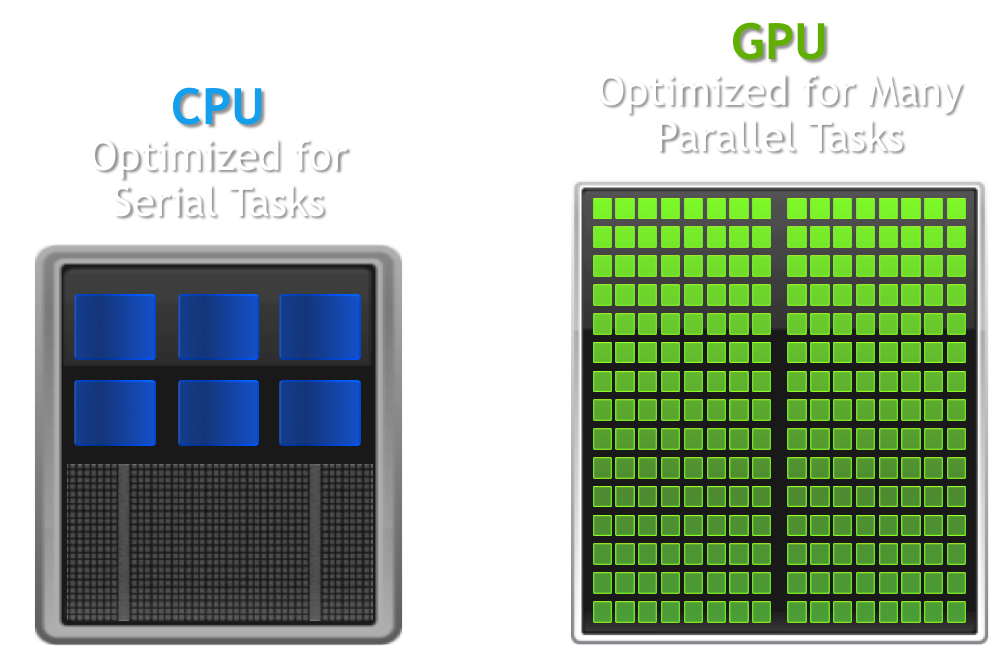
\includegraphics[width=\linewidth]{figures/cpu_vs_gpu.png}
\caption[Comparison of processor architectures]{Comparison of processor architectures: CPU (left) and GPU (right) differ tremendously in the number of ALUs packed on a chip [\url{https://www.datascience.com/blog/cpu-gpu-machine-learning}]}
\label{fig:gpu-comparison}
\end{figure}

MATLAB makes processing data using the GPU seemingly trivial by overloading a large number of built in functions.
Performance varies however.
Writing a kernel-type subfunction is often the fastest way to implement a routine written as if it operates on single (scalar) element only that can be called on all pixels at once or employs all pixel-subscripts used by the function to retrieve the pixel value at a given subscript.
The kernel-type function is compiled into a CUDA kernel the first time it's called, then repeated calls directly contact the kernel with minimal overhead.
Calls typically use the arrayfun() function.

Data transfers between system memory and graphics memory is often a major bottle-neck.
Therefore, this operation is best performed only once.
However, once data is available to the GPU, many complex operations can be performed to extract information from the image without exceeding the processing-time limit imposed by the frame-rate of the camera sending the images.

In total, this project employs advances in both software and hardware that facilitate rapid accurate image analysis of living organisms with the ultimate goals of simplifying the acquisition and analysis of neural activity indicators in both normal and pathological states.

% \clearpage

% \end{document}

\clearpage{}


% CHAPTER 2: THE BODY OF THESIS
\documentclass[../main.tex]{subfiles}
\begin{document}

\thispagestyle{myheadings}

\chapter{Neural Interfaces: Fabrication, programming, and assembly}
\label{sec:neural-interfaces}

This chapter describes several projects that were started early during my graduate studies.
Each project is similar in that they are outside the realm of optical imaging of neural activity, which is the focus of the rest of this dissertation.
Nevertheless, they are included here because the issues they bring up will later inform the approach I take in the work described in later chapters.
The projects described in the following sections are also tied together by a common goal: to enable research in the neurosciences with translation potential for clinical applications.

\section{Animal Tracking}\label{sec:animal-tracking}

\subsection{PD mouse model:}\label{sec:pd-mouse-model}

You can induce a quantifiable PD-like state in mice with a unilateral injection of the neurotoxin 6-hydroxydopamine (6-OHDA) into the striatum, and subsequent administration of apomorphine to provoke side-biased motor deficits \cite{iancu_behavioral_2005}
Side-biased ``turning'' behavior is quantified autonomously on two distinct platforms, a computer-vision system that allows free movement, and a virtual-reality spherical treadmill platform that simulates free movement.

\subsection{Metrics of Behavior}\label{sec:metrics-of-behavior}

Two testing platforms are used to assess changes in behavior over time.
Behavior is analyzed and quantified in real-time, and are synchronized with electrophysiology and made available as stream of events synchronized with imaging and/or electrophysiology.
The quantification routine creates a signal that is representative of symptom severity.
For our unilaterally lesioned mouse model of PD the most readily observable impairment is the inability to walk straight;
mice would turn in circles
contralateral to the lesion when given intraperitoneal apomorphine.

\subsection{Behavior Box}\label{sec:behavior-box}

I built an experiment apparatus for mice to enable a study being run by Jia-Min Zhuo.
The goal of the study was to elucidate the role of adult-born neurons on mouse behavior, specifically their performance in discrimination tasks.
We called the apparatus the ``Behavior Box'' and modeled it after a commercially available but grossly over-priced box that itself came from other labs (see \cite{McLelland2015}).
%\cite{creer2010}

The chamber was constructed with black plastic walls, extruded aluminum framing, and a perforated metal mesh floor 1 cm above a plastic waste tray.
A 10-inch infrared touchscreen (ITouch Systems) was mounted over a 10-inch LCD monitor forming one wall of the chamber.
An opaque mask with seven windows was placed over the screen to limit where the mouse could touch.
A water pump with infrared detector was located at the other end of the chamber to provide reward for the water-deprived mice in the study.
A white LED strip encircled the chamber from the top, and multiple speakers positioned outside to deliver sound cues.
A web camera was fixed above the chamber to record and monitor mouse activity.
My contribution to this project was the program that facilitated interaction between all the system components.
This program controlled and recorded experiment progress.
I developed the program in MATLAB, and the main components of its function are described below.
This system would eventually be used for a study investigating the development of adult-born neurons in the hippocampus (\cite{Zhuo_2016}).

\begin{figure}
	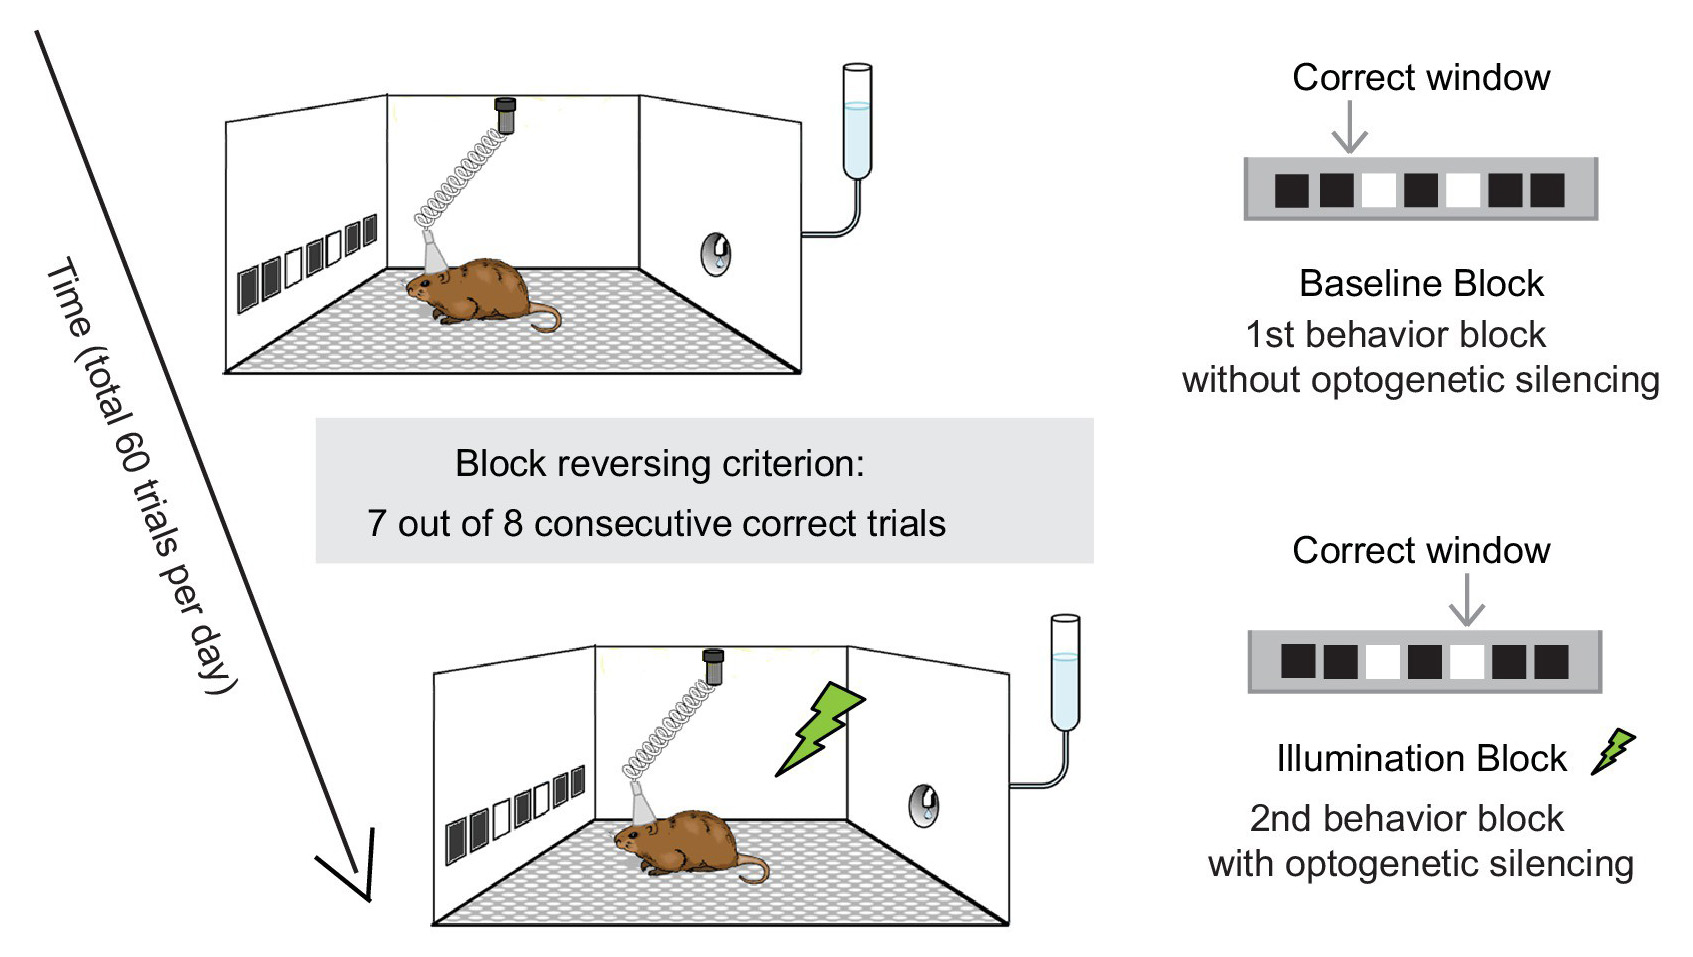
\includegraphics[width=15cm]{task-schematic.jpg}
	\caption{behavior-box schematic}
	\label{fig:behaivorbox schematic}
\end{figure}

\subsection{IR Touchscreen}\label{sec:ir-touchscreen}

The IR touchscreen provided a robust measure of the location of any contact with the animal's paws or nose.
The screen was more reliable than either \emph{resistive} or \emph{capacitive} touchscreens, which are much more common in devices like POS systems and mobile phones respectively.

The scientists users interact with the device through command-line manipulation of a ``BehaviorBox'' object in the MATLAB REPL.
This approach provides access to features for easily customizable control of physical components including the infrared touchscreen and LCD display along with speakers, water-ports, lights, essentially anything that can be controlled electronically.
The approach also enables suggestions and autocomplete options for users new to the environment.

\subsection{FrameSynx Toolbox}\label{sec:framesynx-toolbox}

The FrameSynx toolbox for MATLAB was built to synchronize continuous image acquisition with experiments conducted in the neuroscience laboratory setting.
While the experiments are conducted in separate software (and potentially on a different computer), FrameSynx listens for messages to start/stop the experiment, start a trial, etc. and responds accordingly by controlling one or multiple cameras and illumination devices, and synchronizing this information with the data acquired.
The major contribution to the ``Behavior Box'' package, and also to later image processing packages is the procedure for definition and storage and of experimental data files, which will be touched on briefly in chapter 3.
% todo

\subsection{Using Computer Vision to track Position and Orientation}\label{sec:using-computer-vision-to-track-position-and-orientation}

\subsection{Mouse in a Bowl}\label{sec:mouse-in-a-bowl}

A webcam-based motion tracking box constructed to analyze the movement of our unilaterally lesioned PD mouse model.
Video is recorded at 15 frames per second and processed on-line or off-line using a function written in MATLAB.
Briefly, this function converts each frame to a black and white image (logical matrix), uses morphological filtering functions to isolate the mouse (remove mouse excrement) and identify its body (remove the tail), then finds the center of mass in cartesian coordinates (maximum center of projection on x- and y-axes), and the rostral-caudal orientation measured in degrees off the x-axis.
Orientation is determined by the index of maximum of a radon transform of the binary image.
Processing is accomplished at a rate of 15-16 fps, using a single core, or 64 fps using parallel processing on a quad-core processor with multi-threading enabled.
The advantage of this apparatus over the virtual-reality system is that it allows free movement of an untrained mouse, with real-time movement metrics at nearly the same rate as the spherical treadmill.
This apparatus would go on to be used to investigate the oscillatory dynamics of cholinergig interneurons in the striatum and their association with parkinson's-like motor deficits [\cite{Kondabolu_2016}].

\begin{figure}[htb]
	\begin{minipage}[t]{0.32\linewidth}\centering
		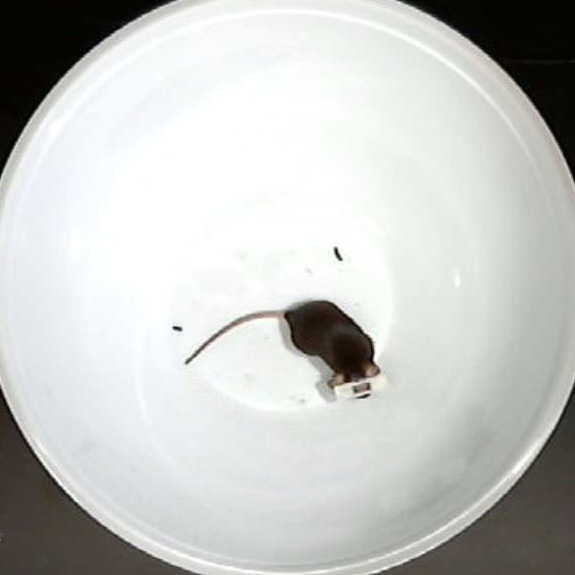
\includegraphics[width=4cm]{01raw.jpg}
		\centerline{(a)}
	\end{minipage}
	\hfill
	\begin{minipage}[t]{0.32\linewidth}\centering
		
\includegraphics[width=4cm]{02black-and-white.jpg}
		\centerline{(b)}
	\end{minipage}
	\begin{minipage}[t]{0.32\linewidth}\centering
		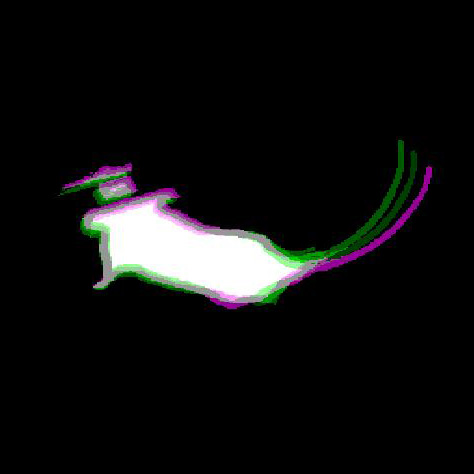
\includegraphics[width=4cm]{03twoframes.jpg}
		\centerline{(c)}
	\end{minipage}
	\caption{
		Automated animal Tracking for ``Mouse in a bowl'' type experiments (a) Raw frame of video being tracked;
		(b) area of detected mouse; (c) overlay of 3 consecutive frames of mouse between each}
	\label{fig:Sampling}
\end{figure}

\begin{figure}[htb]
	\begin{minipage}[t]{0.24\linewidth}\centering
		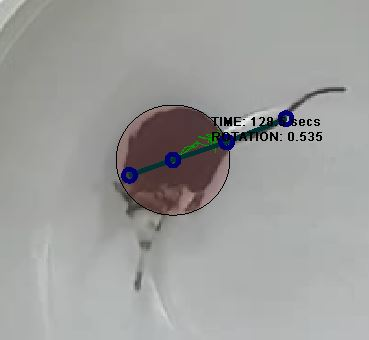
\includegraphics[height=3cm]{07mousedata1close.jpg}
		\centerline{(a)}
	\end{minipage}
	\hfill
	\begin{minipage}[t]{0.24\linewidth}\centering
		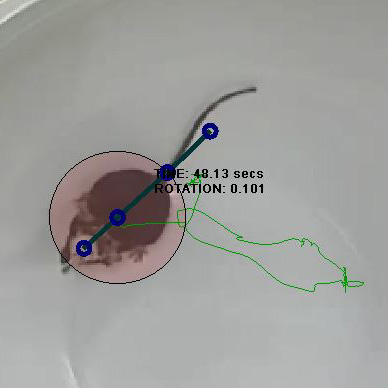
\includegraphics[width=3cm]{06mousedata1.jpg}
		\centerline{(b)}
	\end{minipage}
	\begin{minipage}[t]{0.24\linewidth}\centering
		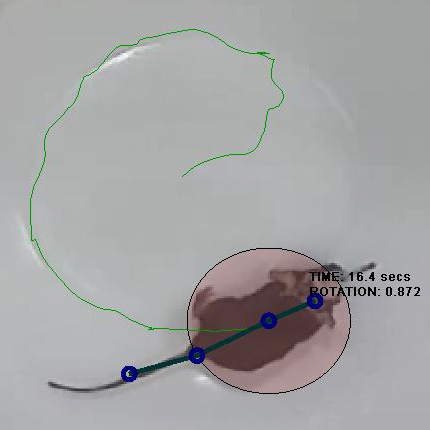
\includegraphics[width=3cm]{08mousedata2.jpg}
		\centerline{(c)}
	\end{minipage}
	\begin{minipage}[t]{0.24\linewidth}\centering
		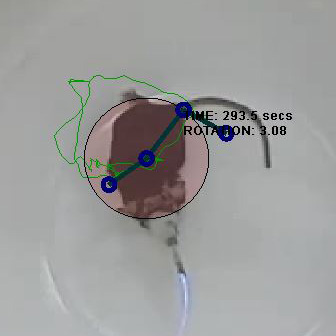
\includegraphics[width=3cm]{09mousedata1fiberon1.jpg}
		\centerline{(d)}
	\end{minipage}
	\caption{
		Automated animal Tracking for ``Mouse in a bowl'' type experiments: (a-d) video overlay showing tracked points} \label{fig:Sampling}
\end{figure}

\subsection{Spherical Treadmill}\label{sec:spherical-treadmill}

A virtual reality system was assembled, adopting methods from the Harvey lab lab \cite{harvey_intracellular_2009}.
This system allows placement of a head-restrained mouse on an 8-inch diameter polystyrene foam ball supported by a cushion of compressed air, surrounded by a toroidal projection screen.
Ball rotation is tracked with two optical computer mice placed orthogonal to each other.
Movement vectors are fed into a virtual-reality engine that updates the image projected onto a toroidal screen surrounding the ball, simulating movement through any arbitrary virtual world.
Movement vectors are recorded as an arbitrarily scaled translation in the mouse-relative X and Y axes and rotation around the Z axis, at approximately 30 ms intervals.
This behavioral apparatus has the advantage of allowing trivial measurement of the mouse's movement ability while the mouse is head-fixed.
The disadvantage is the time and potential confounds involved with training individual mice to use the system.

\begin{figure}[htb]
	\begin{minipage}[t]{0.32\linewidth}\centering
		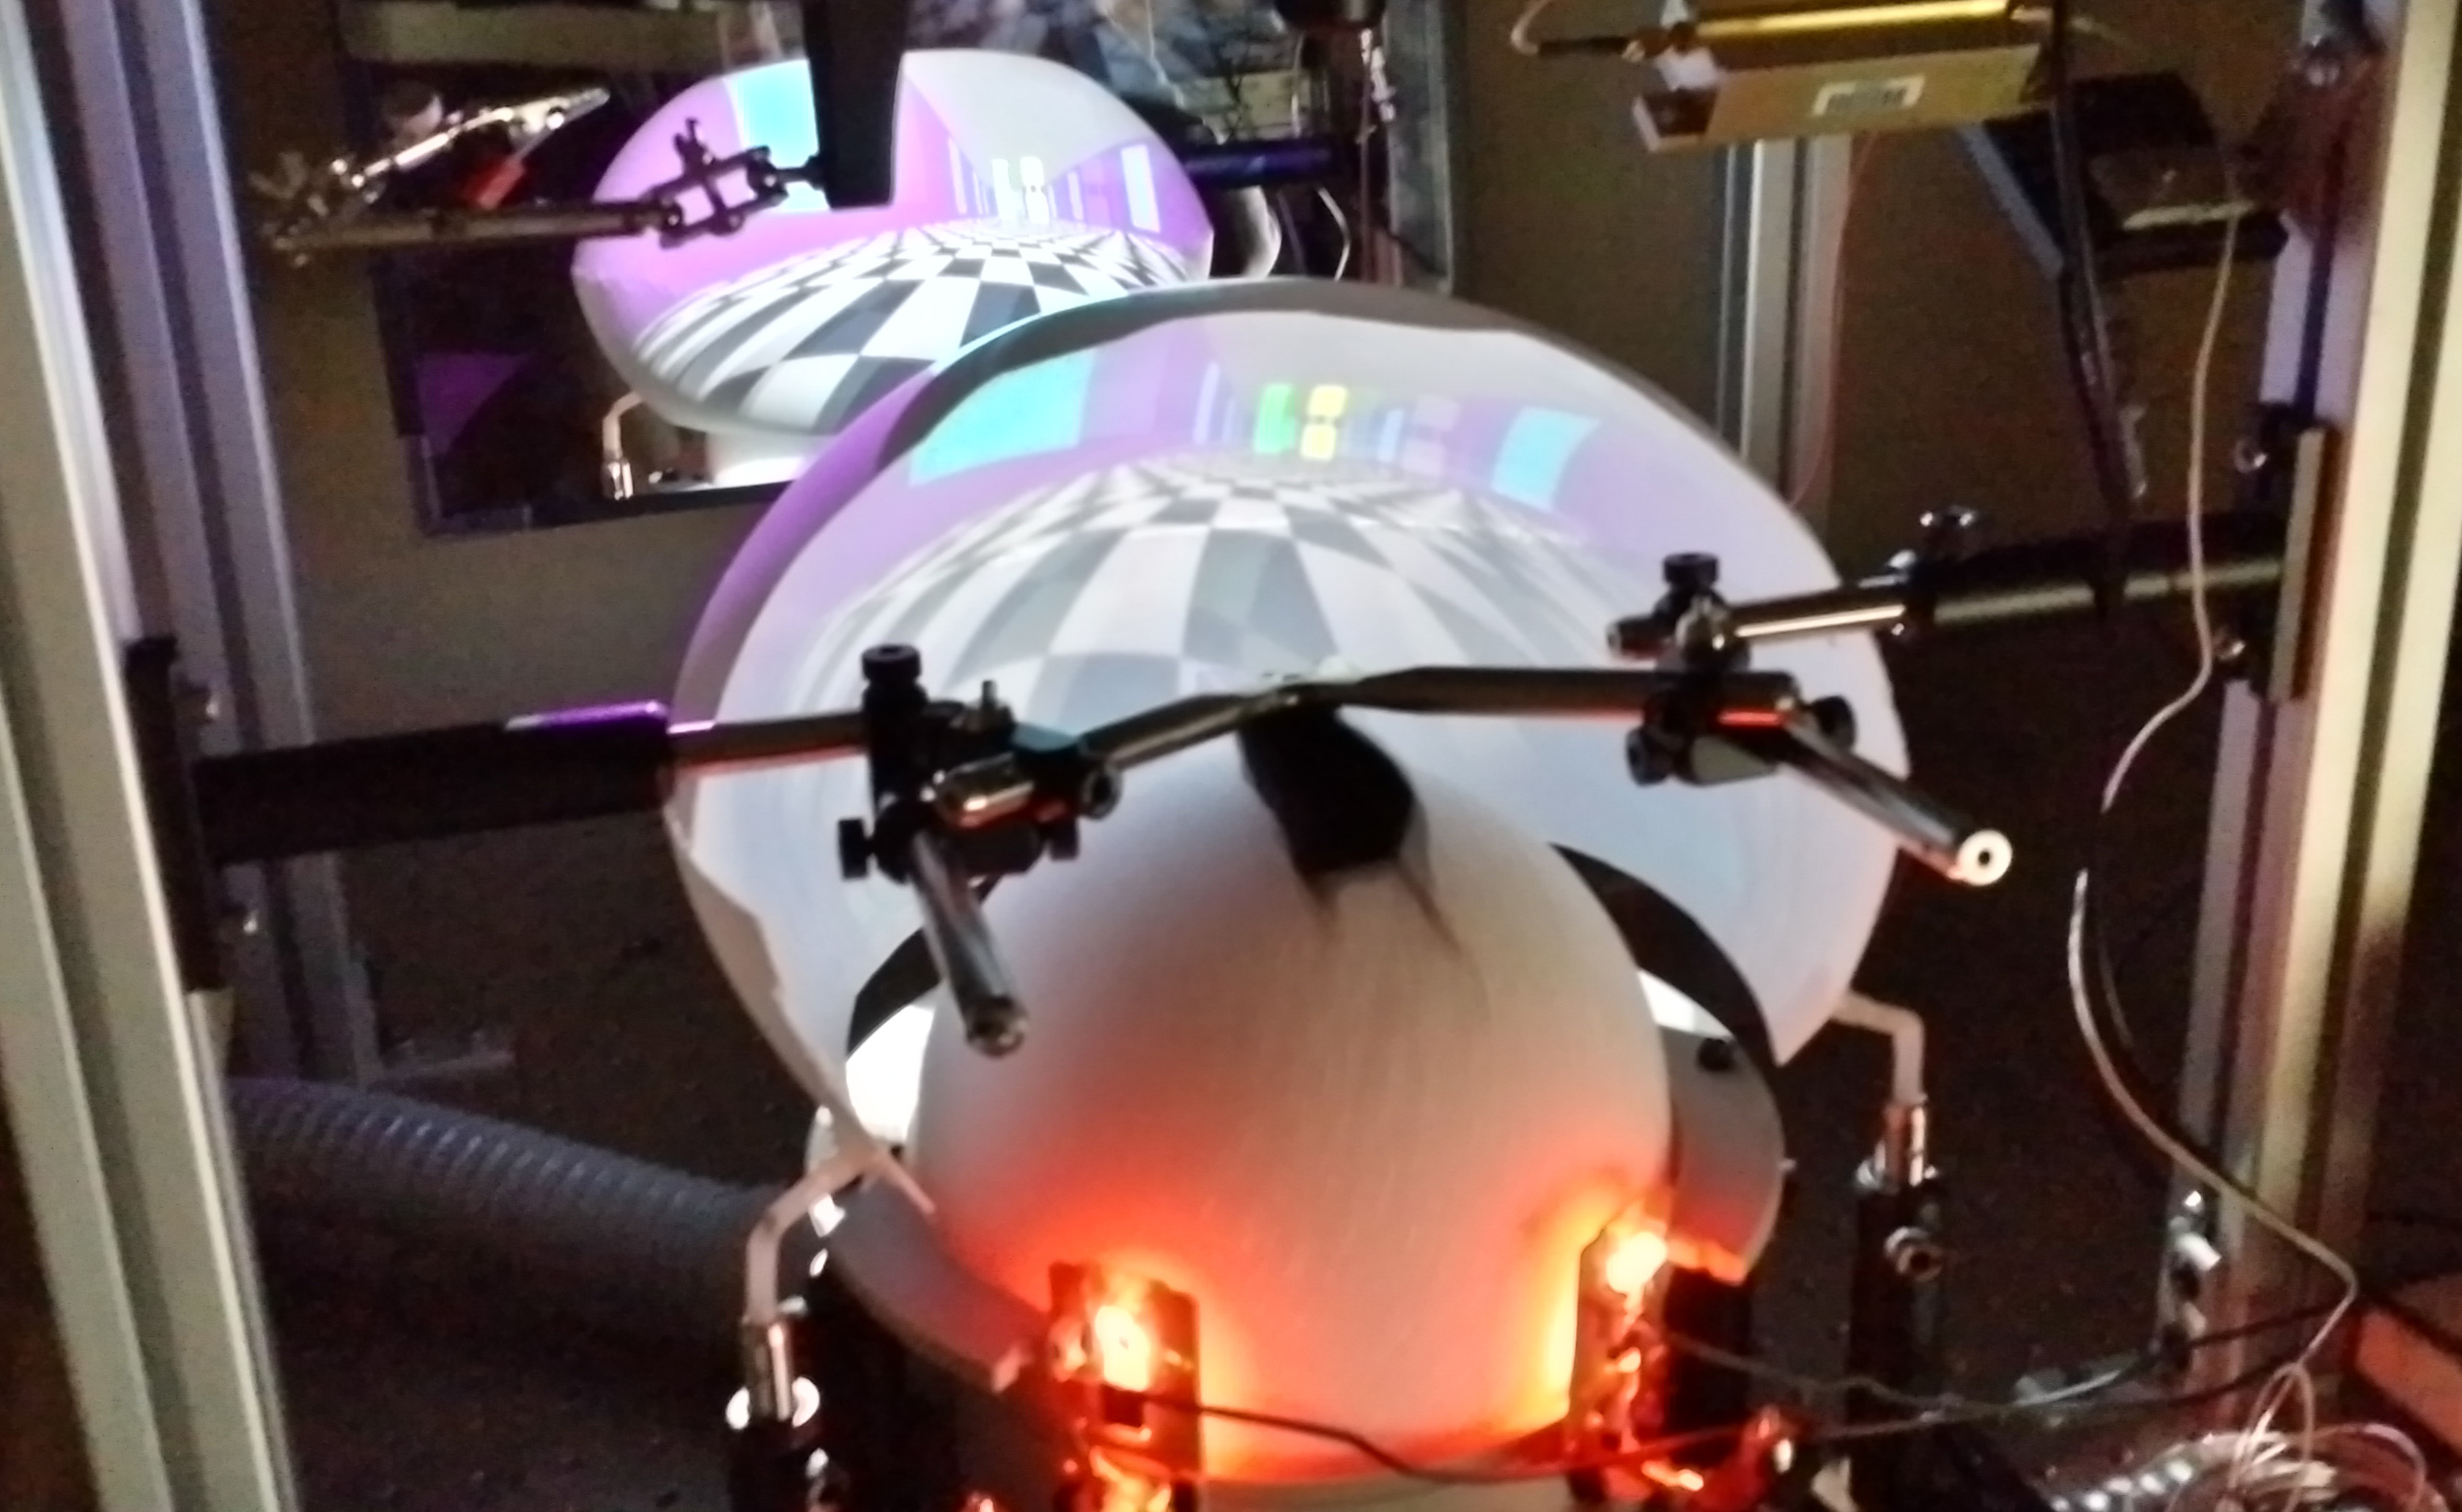
\includegraphics[height=3.5cm]{01-treadmill-mouse-running.jpg}
		\centerline{(a)}
	\end{minipage}
	\hfill
	\begin{minipage}[t]{0.15\linewidth}\centering
		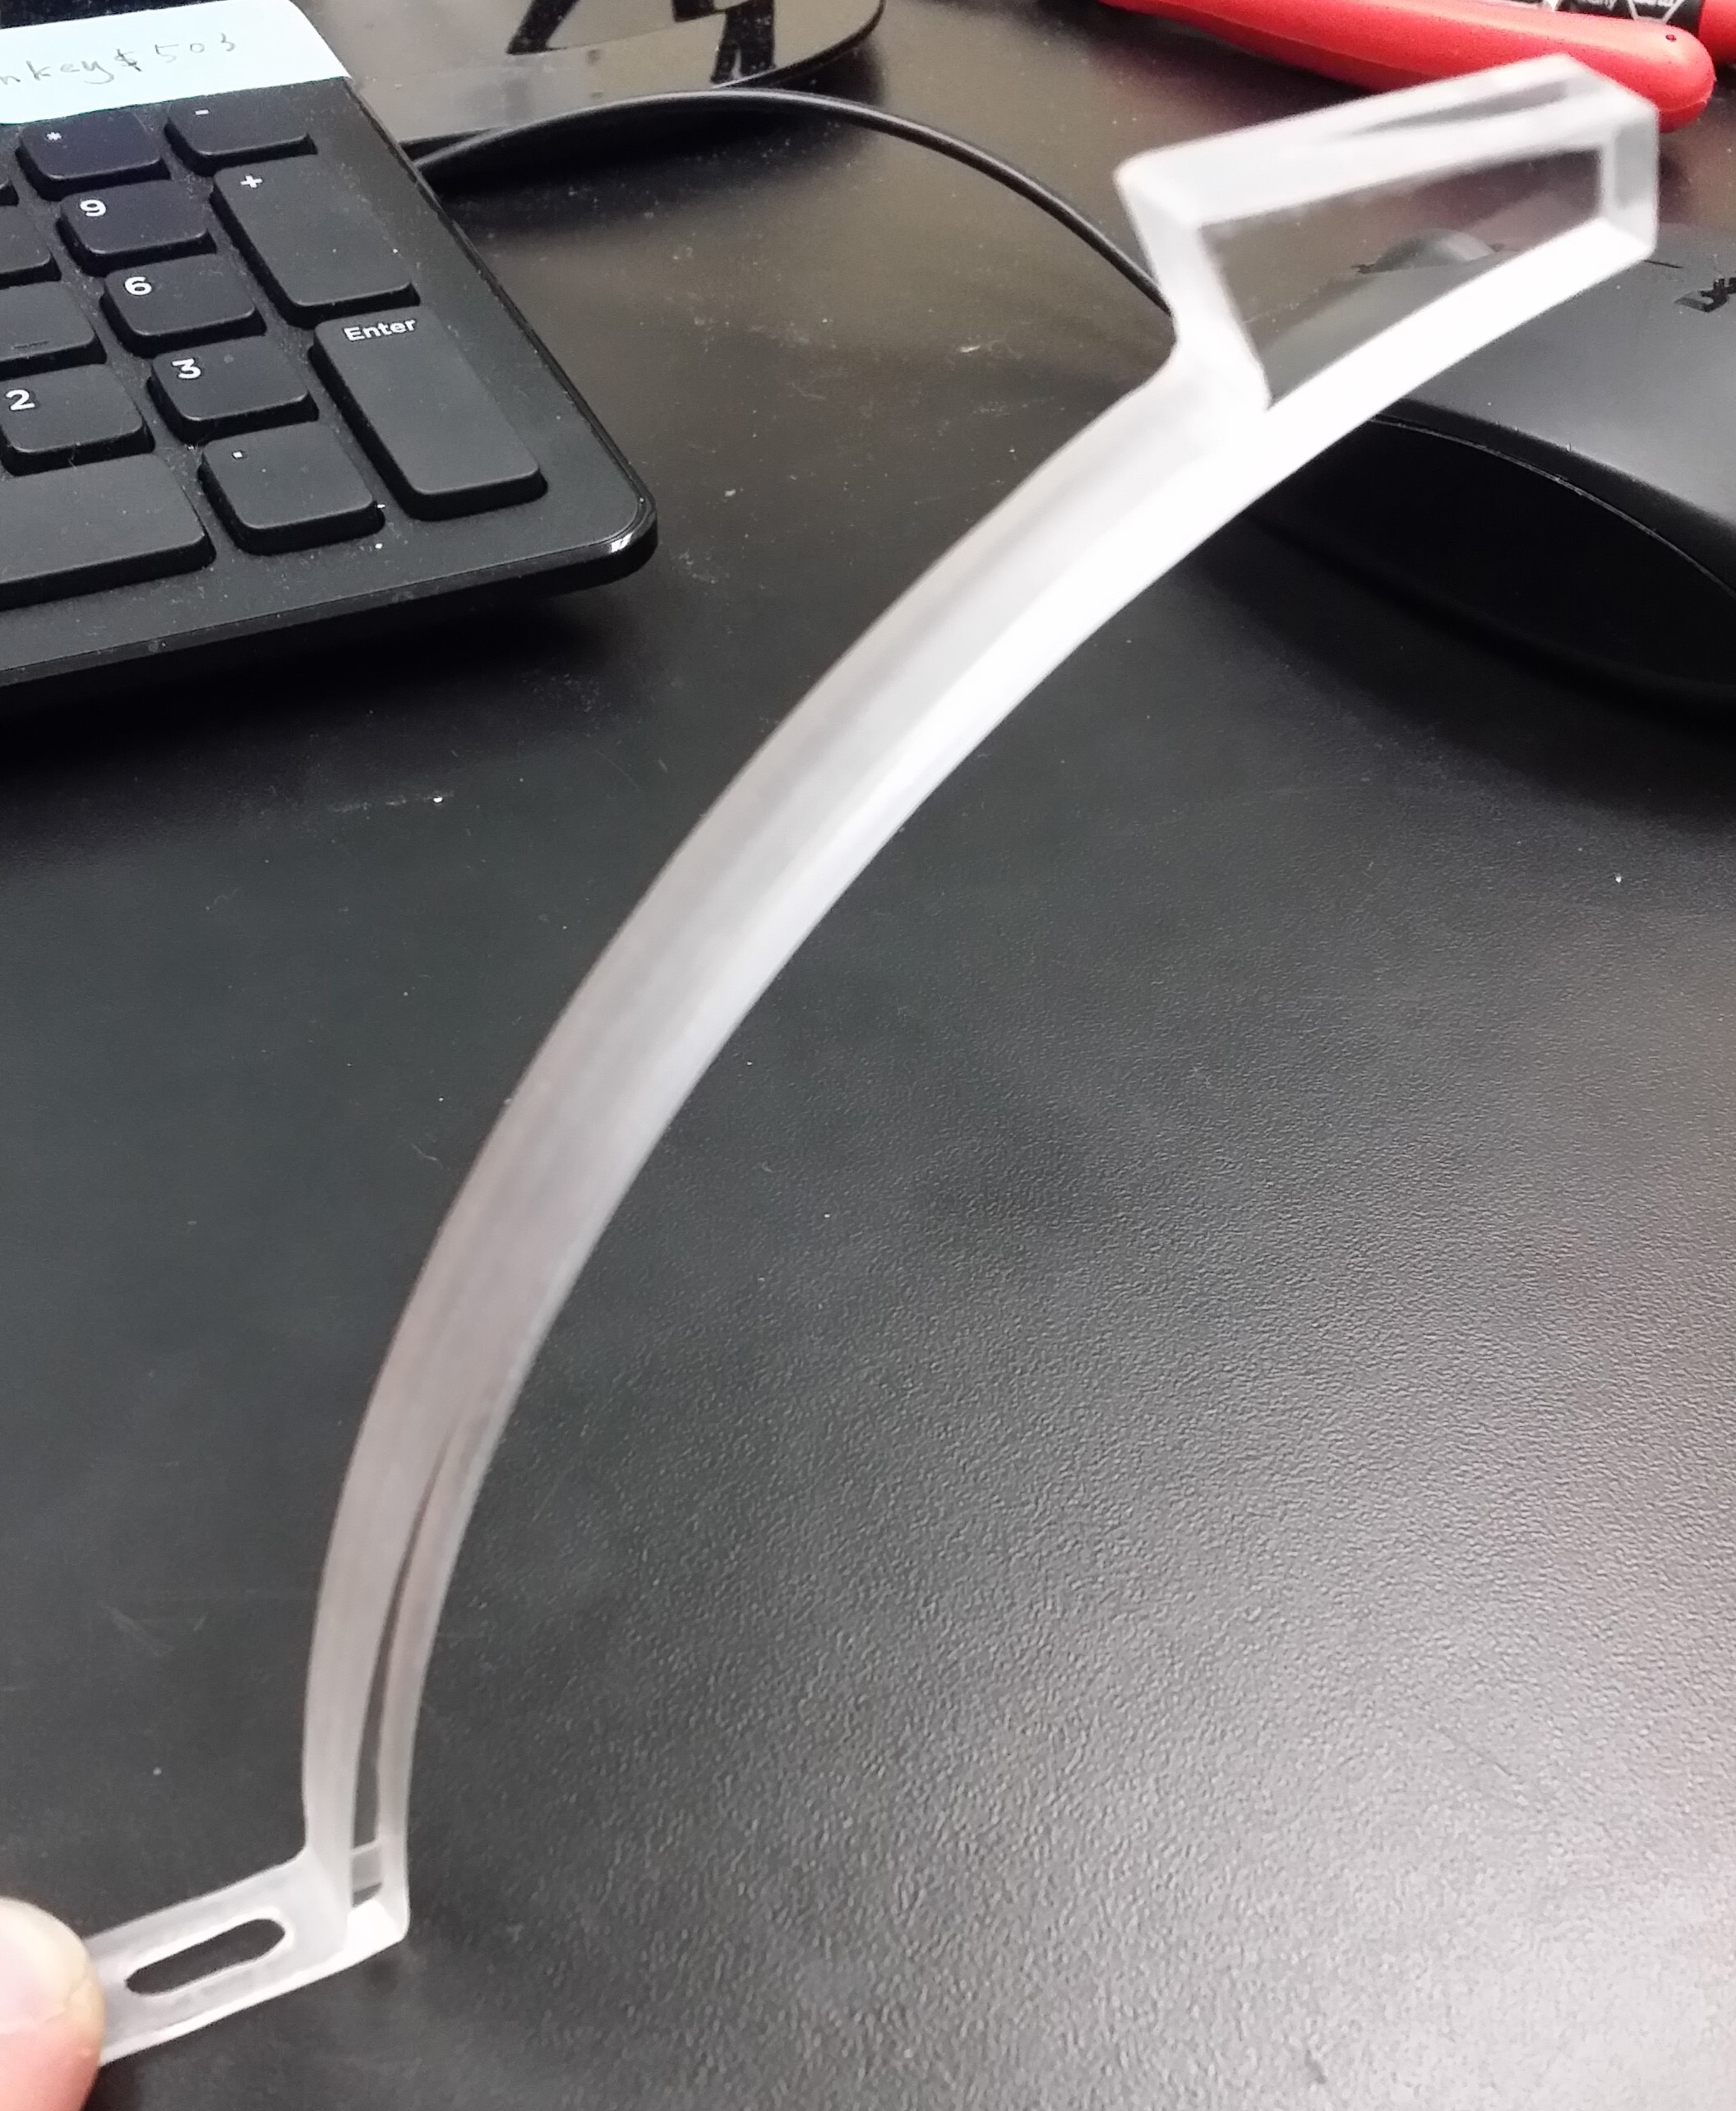
\includegraphics[height=3.5cm]{01-water-port.jpg}
		\centerline{(b)}
	\end{minipage}
	\begin{minipage}[t]{0.45\linewidth}\centering
		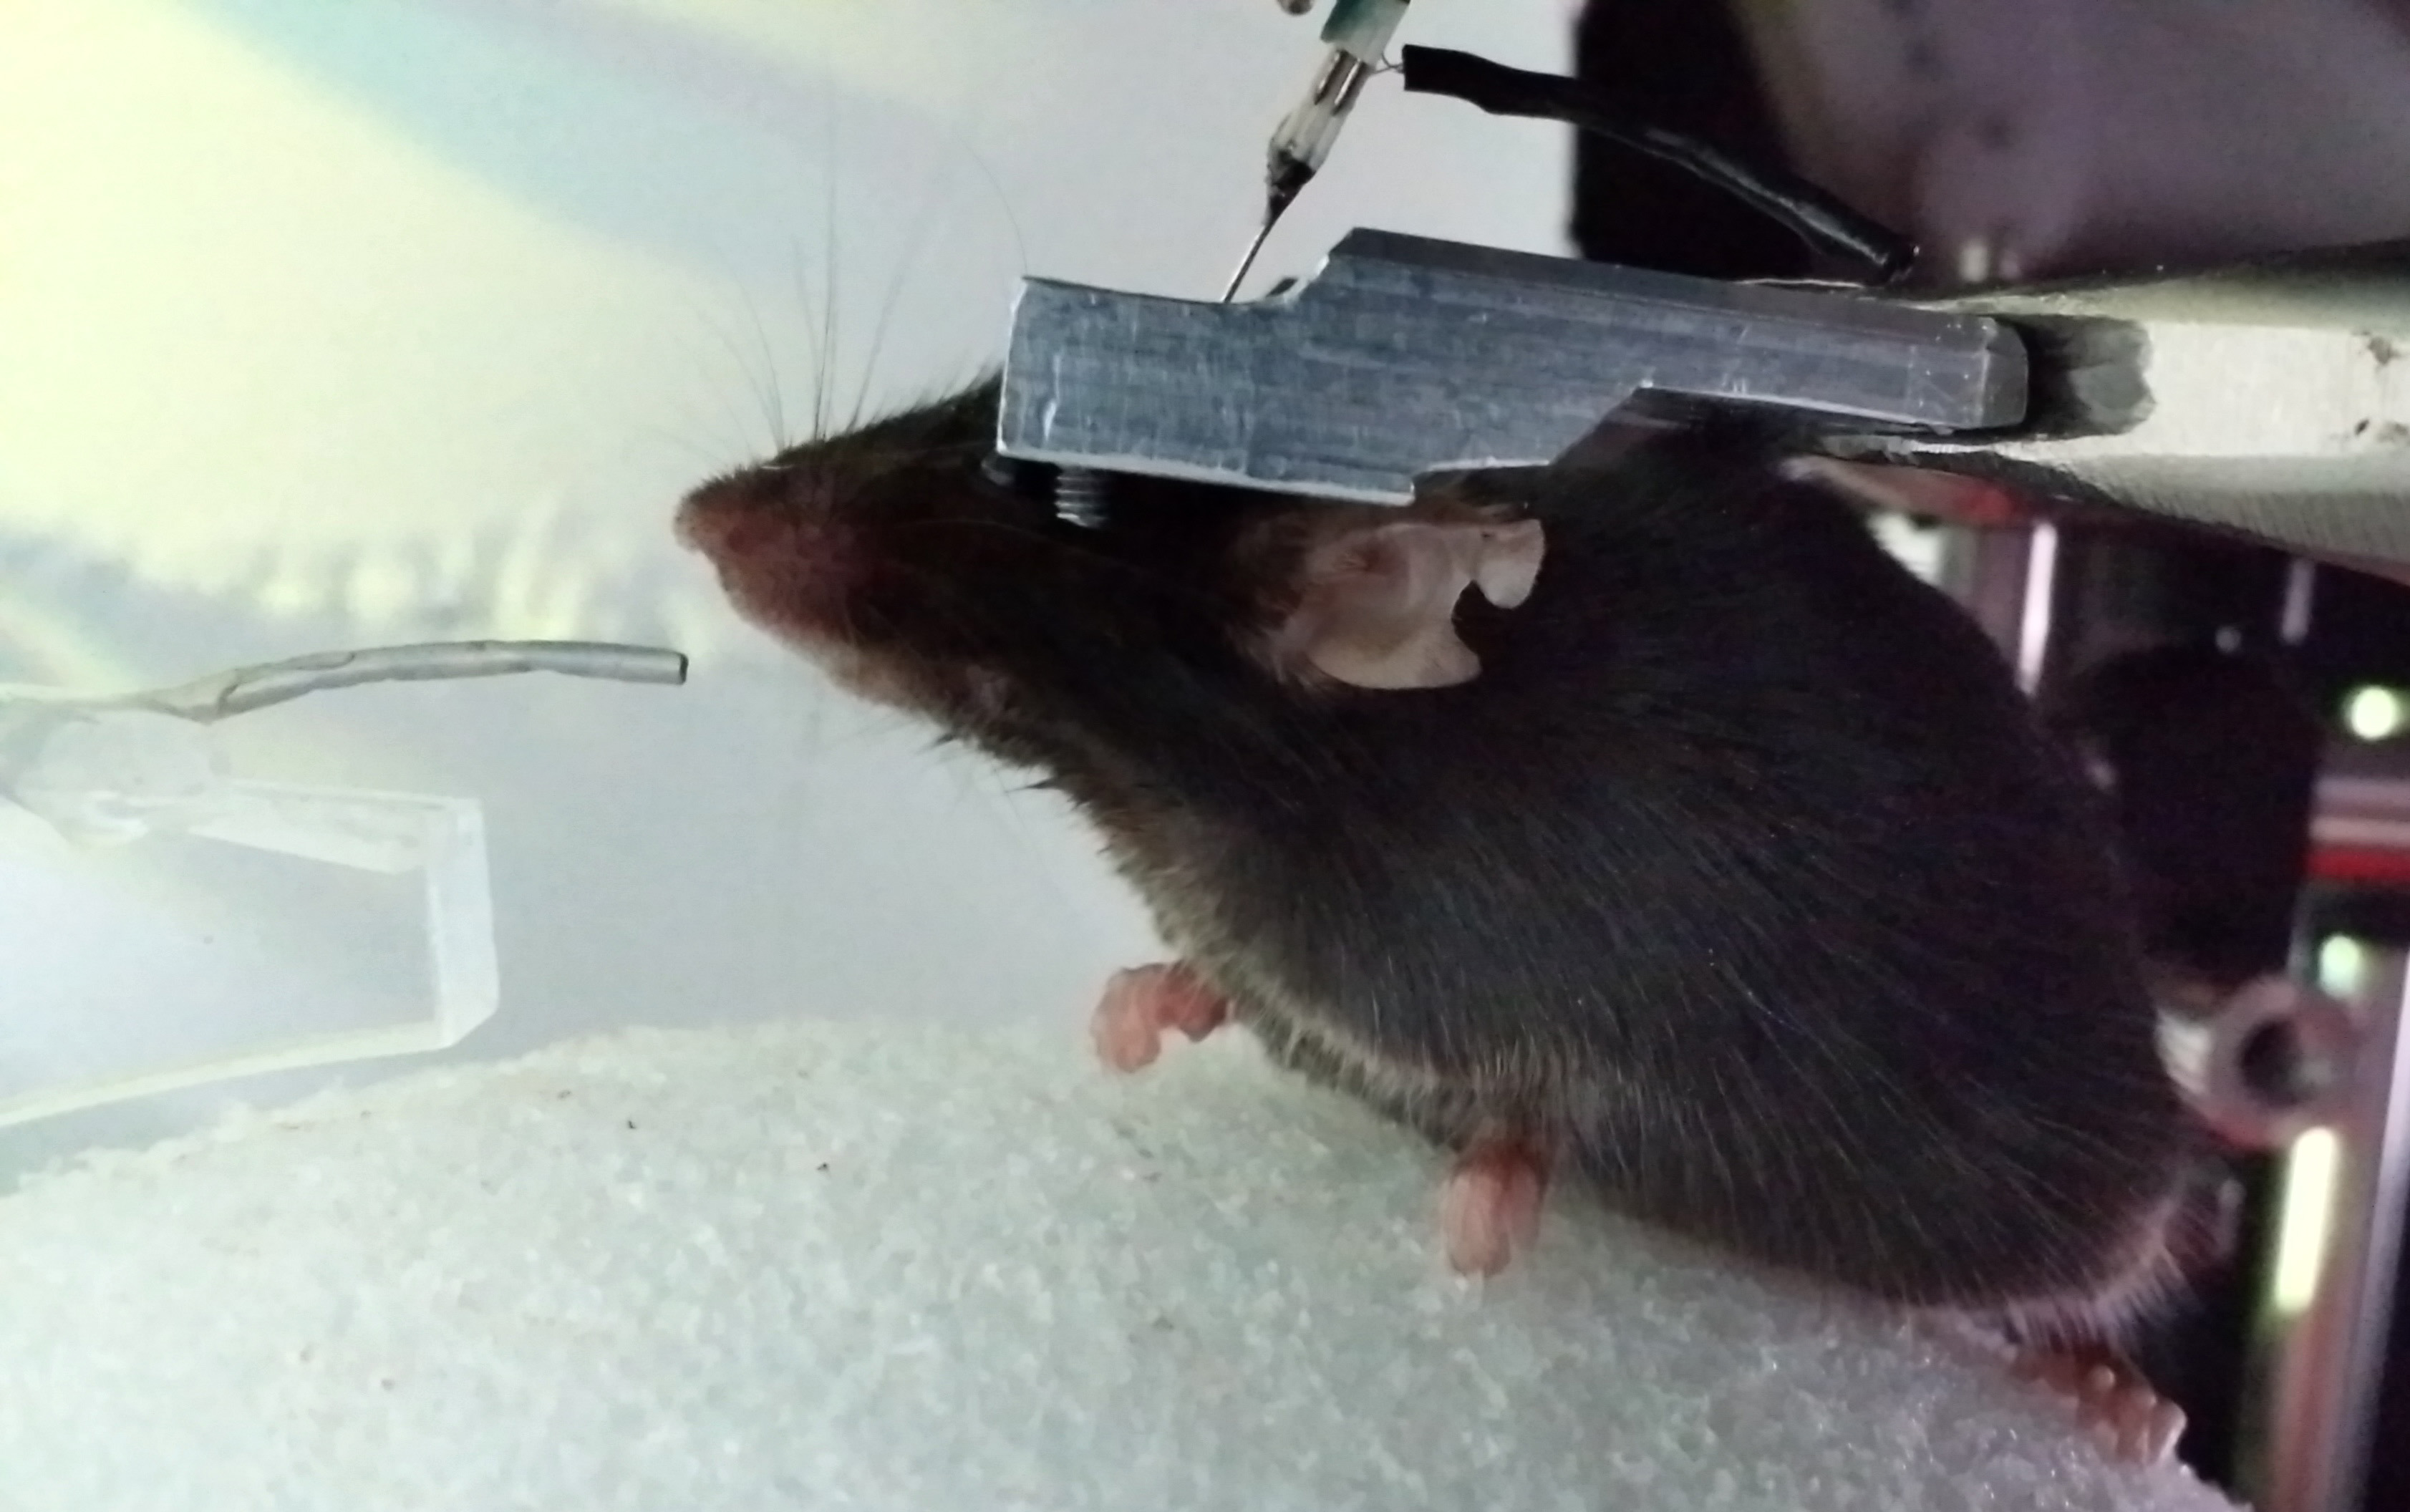
\includegraphics[height=3.5cm]{03-water-delivery-zoom.jpg}
		\centerline{(c)}
	\end{minipage}
	\caption{
		Spherical treadmill (a) Mouse running on a treadmill equpipped with virtual reality;
		(b) water port; (c) application of the water delivery system }
	\label{fig:Spherical treadmill}
\end{figure}

\subsection{Headplate Holder}\label{sec:headplate-holder}

\begin{figure}[htb]
	\begin{minipage}[t]{0.32\linewidth}\centering 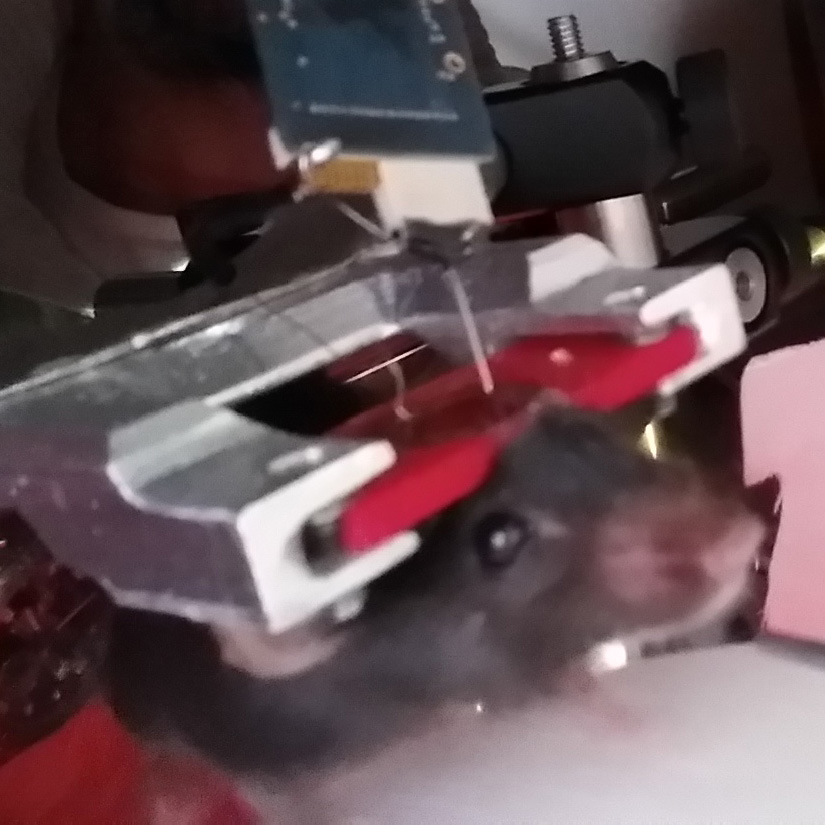
\includegraphics[width=4.5cm]{photo-front.jpg} \centerline{(a)}
	\end{minipage}
	\hfill
	\begin{minipage}[t]{0.32\linewidth}\centering 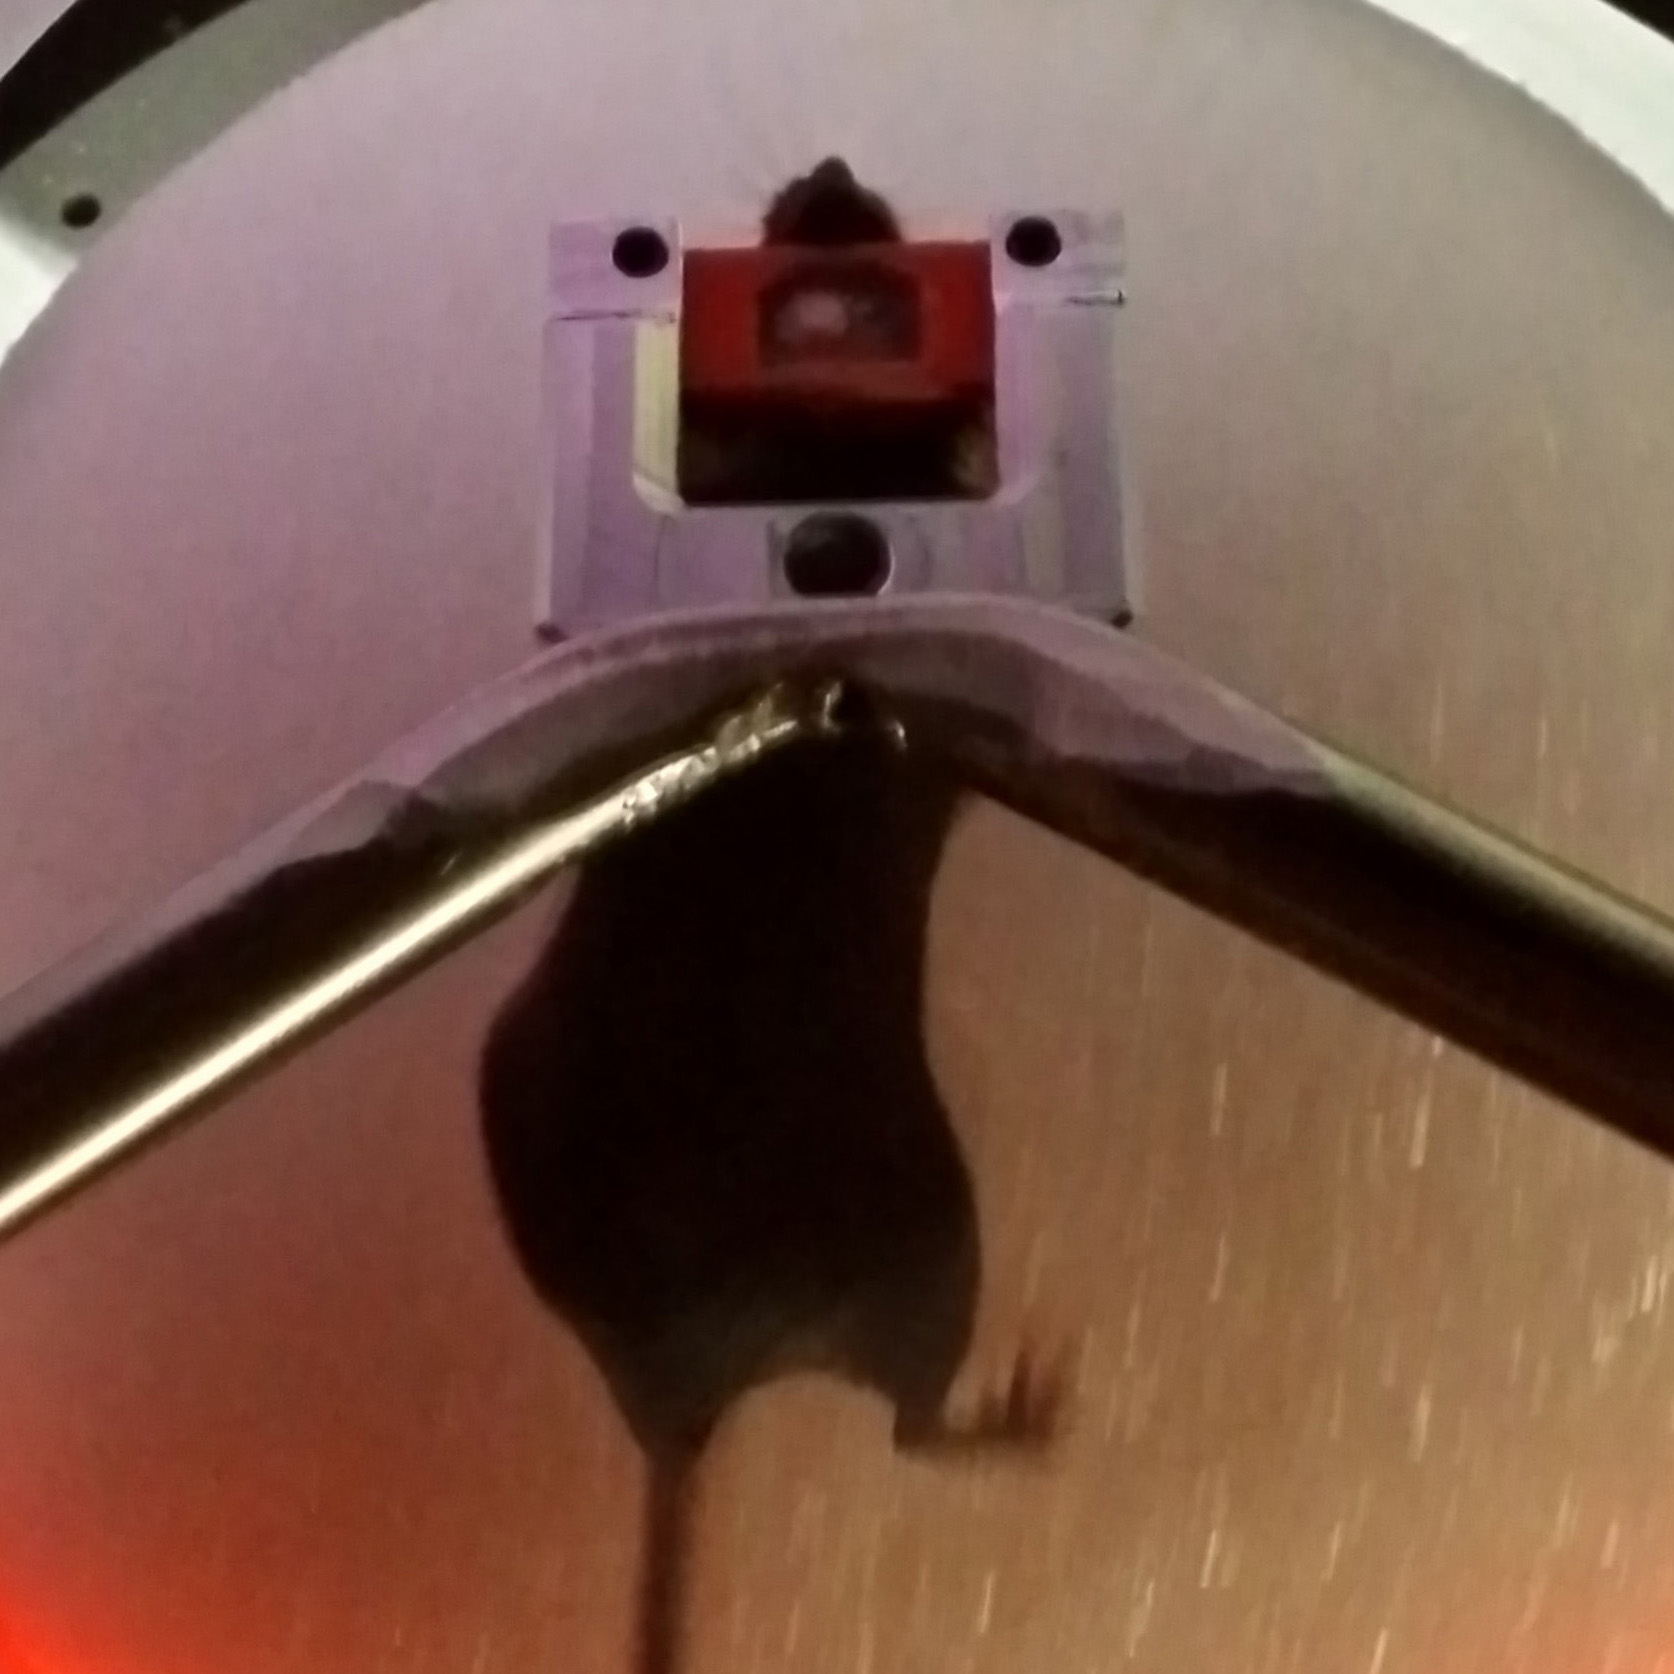
\includegraphics[width=4.5cm]{photo-top.jpg} \centerline{(b)}
	\end{minipage}
	\begin{minipage}[t]{0.32\linewidth}\centering 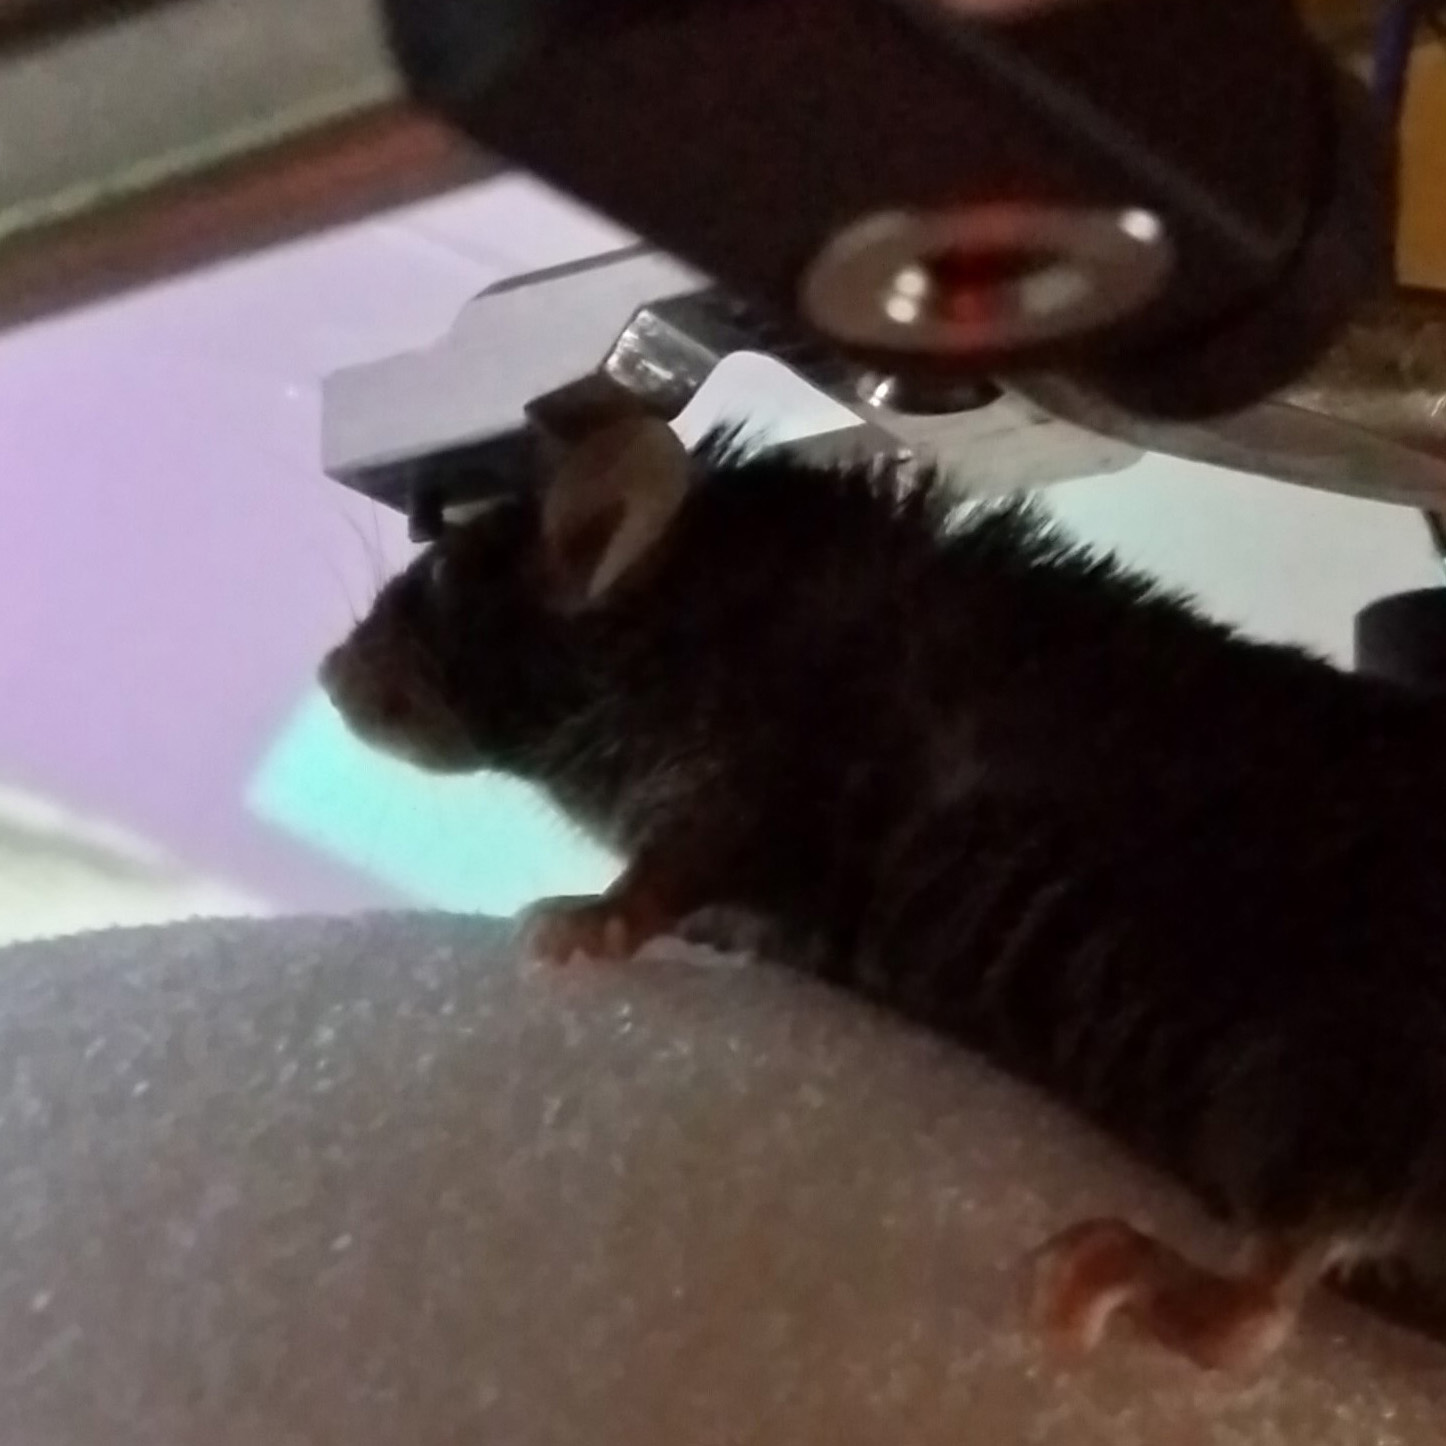
\includegraphics[width=4.5cm]{photo-bottom.jpg} \centerline{(c)}
	\end{minipage}
	\caption{Headplate holder (a) front view;
		(b) top view; (c) bottom view}
	\label{fig:Spherical treadmill}
\end{figure}

\subsection{Motion Sensors}\label{sec:motion-sensors}

Motion sensing was implemented using a linux computer and standard mice at first, and later using precision laser navigation sensors for ``gaming'' mice and custom firmware written to work with any arduino-compatible microcontroller.

\subsection{Generic USB Computer Mouse with Minimal Linux}\label{sec:generic-usb-computer-mouse-with-minimal-linux}

Run ``mouse\_relay.py'' on any computer running linux to send xy-data from 2 USB optical computer mice to another computer over an RS-232 serial-port connection.
The receiving computer (in this implementation) uses MATLAB to read the values and translate the xy-values from 2 mice on the surface of a sphere into 3 values corresponding to rotation of that sphere around 3 orthogonal axes (XYZ) with their origin at the sphere's center.

RECEIVING FUNCTIONS: The MATLAB class that receives the serial input (xy-values from both mice) is called ``VrMovementInterface''

The MATLAB function that translates the double-stream of xy-values from the sphere's surface into rotation around its center is called ``moveBucklin.m'' and is located in the VIRMEN ``movements'' folder.

SERIAL FORMAT: XY-Values are transmitted in `packets' using an ascii formatted string terminated by a newline.
Each packet contains the Sensor Number (s) that the reading is coming from, followed by the X-Value (dx), then the Y-Value (dy).
The python code looks like the following:

A single reading is received at the other end of the serial connection looking something like the following:

\begin{quote}
	s1x34y-3
\end{quote}

\subsection{Navigation Sensor Chip with Arduino}\label{sec:navigation-sensor-chip-with-arduino}

The system was later improved.
%\begin{Shaded}%\begin{Highlighting}[]%\NormalTok{> datastring = s + }\StringTok{'x'}\NormalTok{+dx + %}\StringTok{'y'}\NormalTok{+dy + %}\StringTok{'}\CharTok{\textbackslash{}n}\StringTok{'}%\end{Highlighting}%\end{Shaded}
Works with ADNS library to pass {[}dx,dy{]} measurements from two ADNS-9800 laser mouse sensors (placed 45-degrees apart on surface of Styrofoam ball).

\begin{figure}[htb]
	\begin{minipage}[t]{0.45\linewidth}\centering
		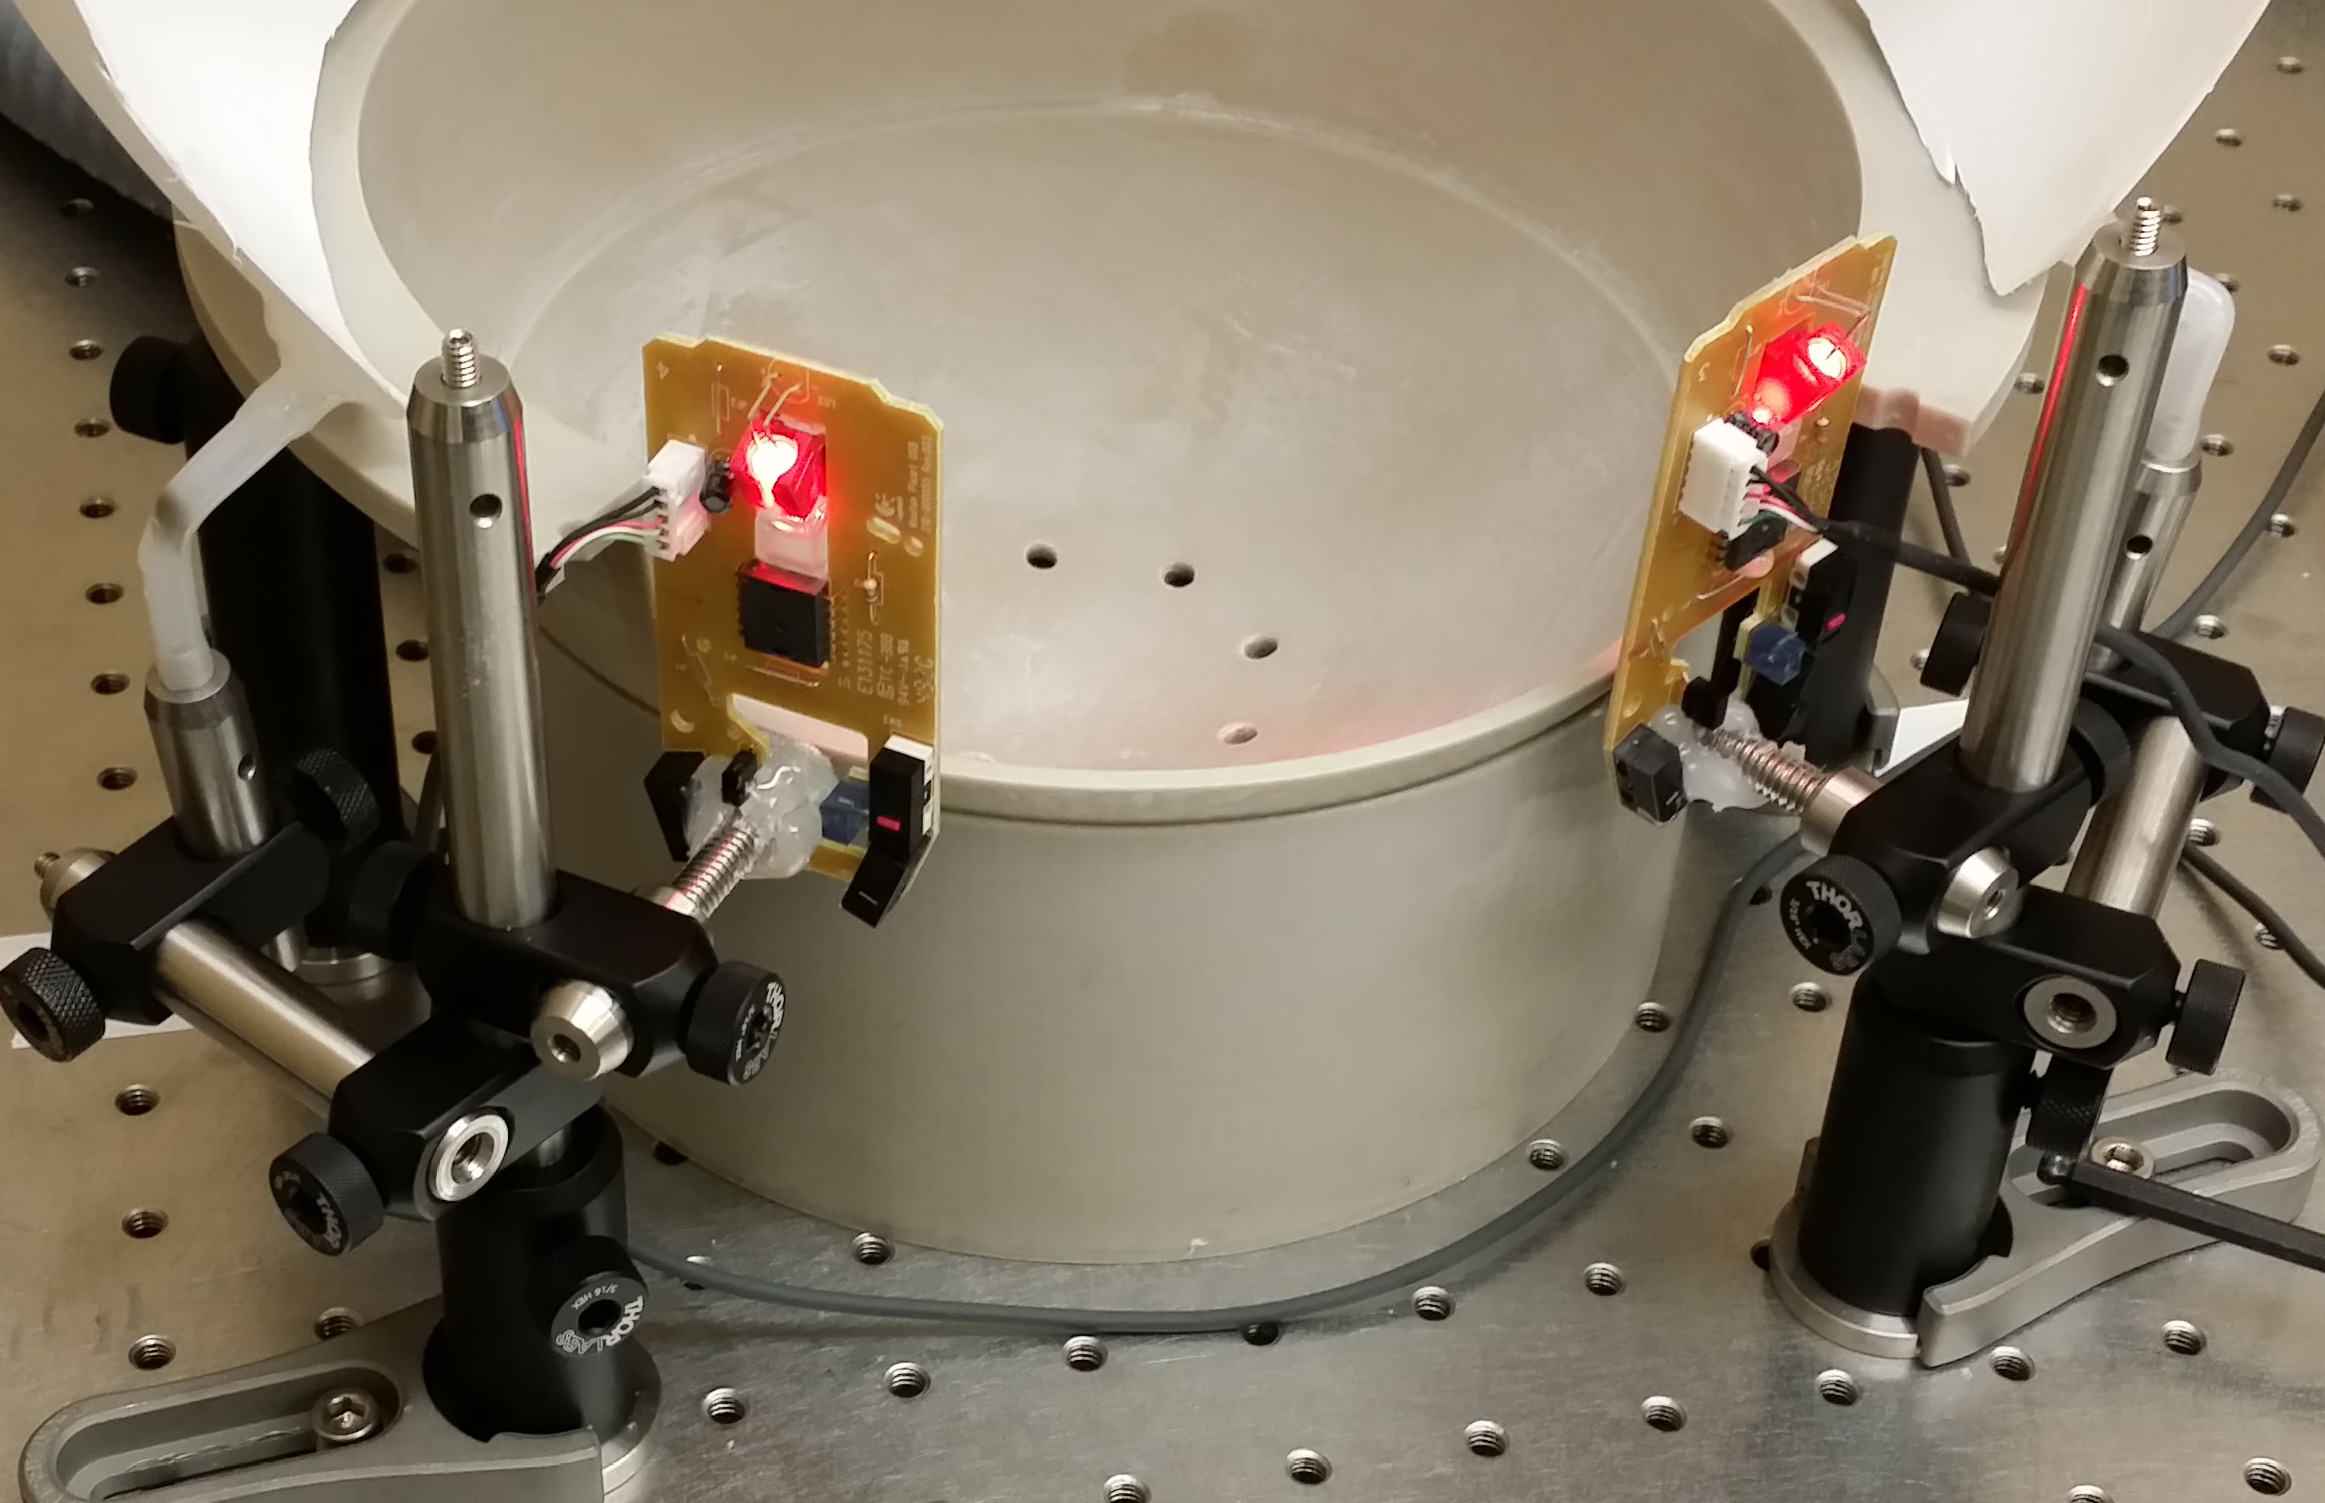
\includegraphics[height=4.5cm]{01-motion-sensors-installed.jpg}
		\centerline{(a)}
	\end{minipage}
	\hfill
	\begin{minipage}[t]{0.45\linewidth}\centering
		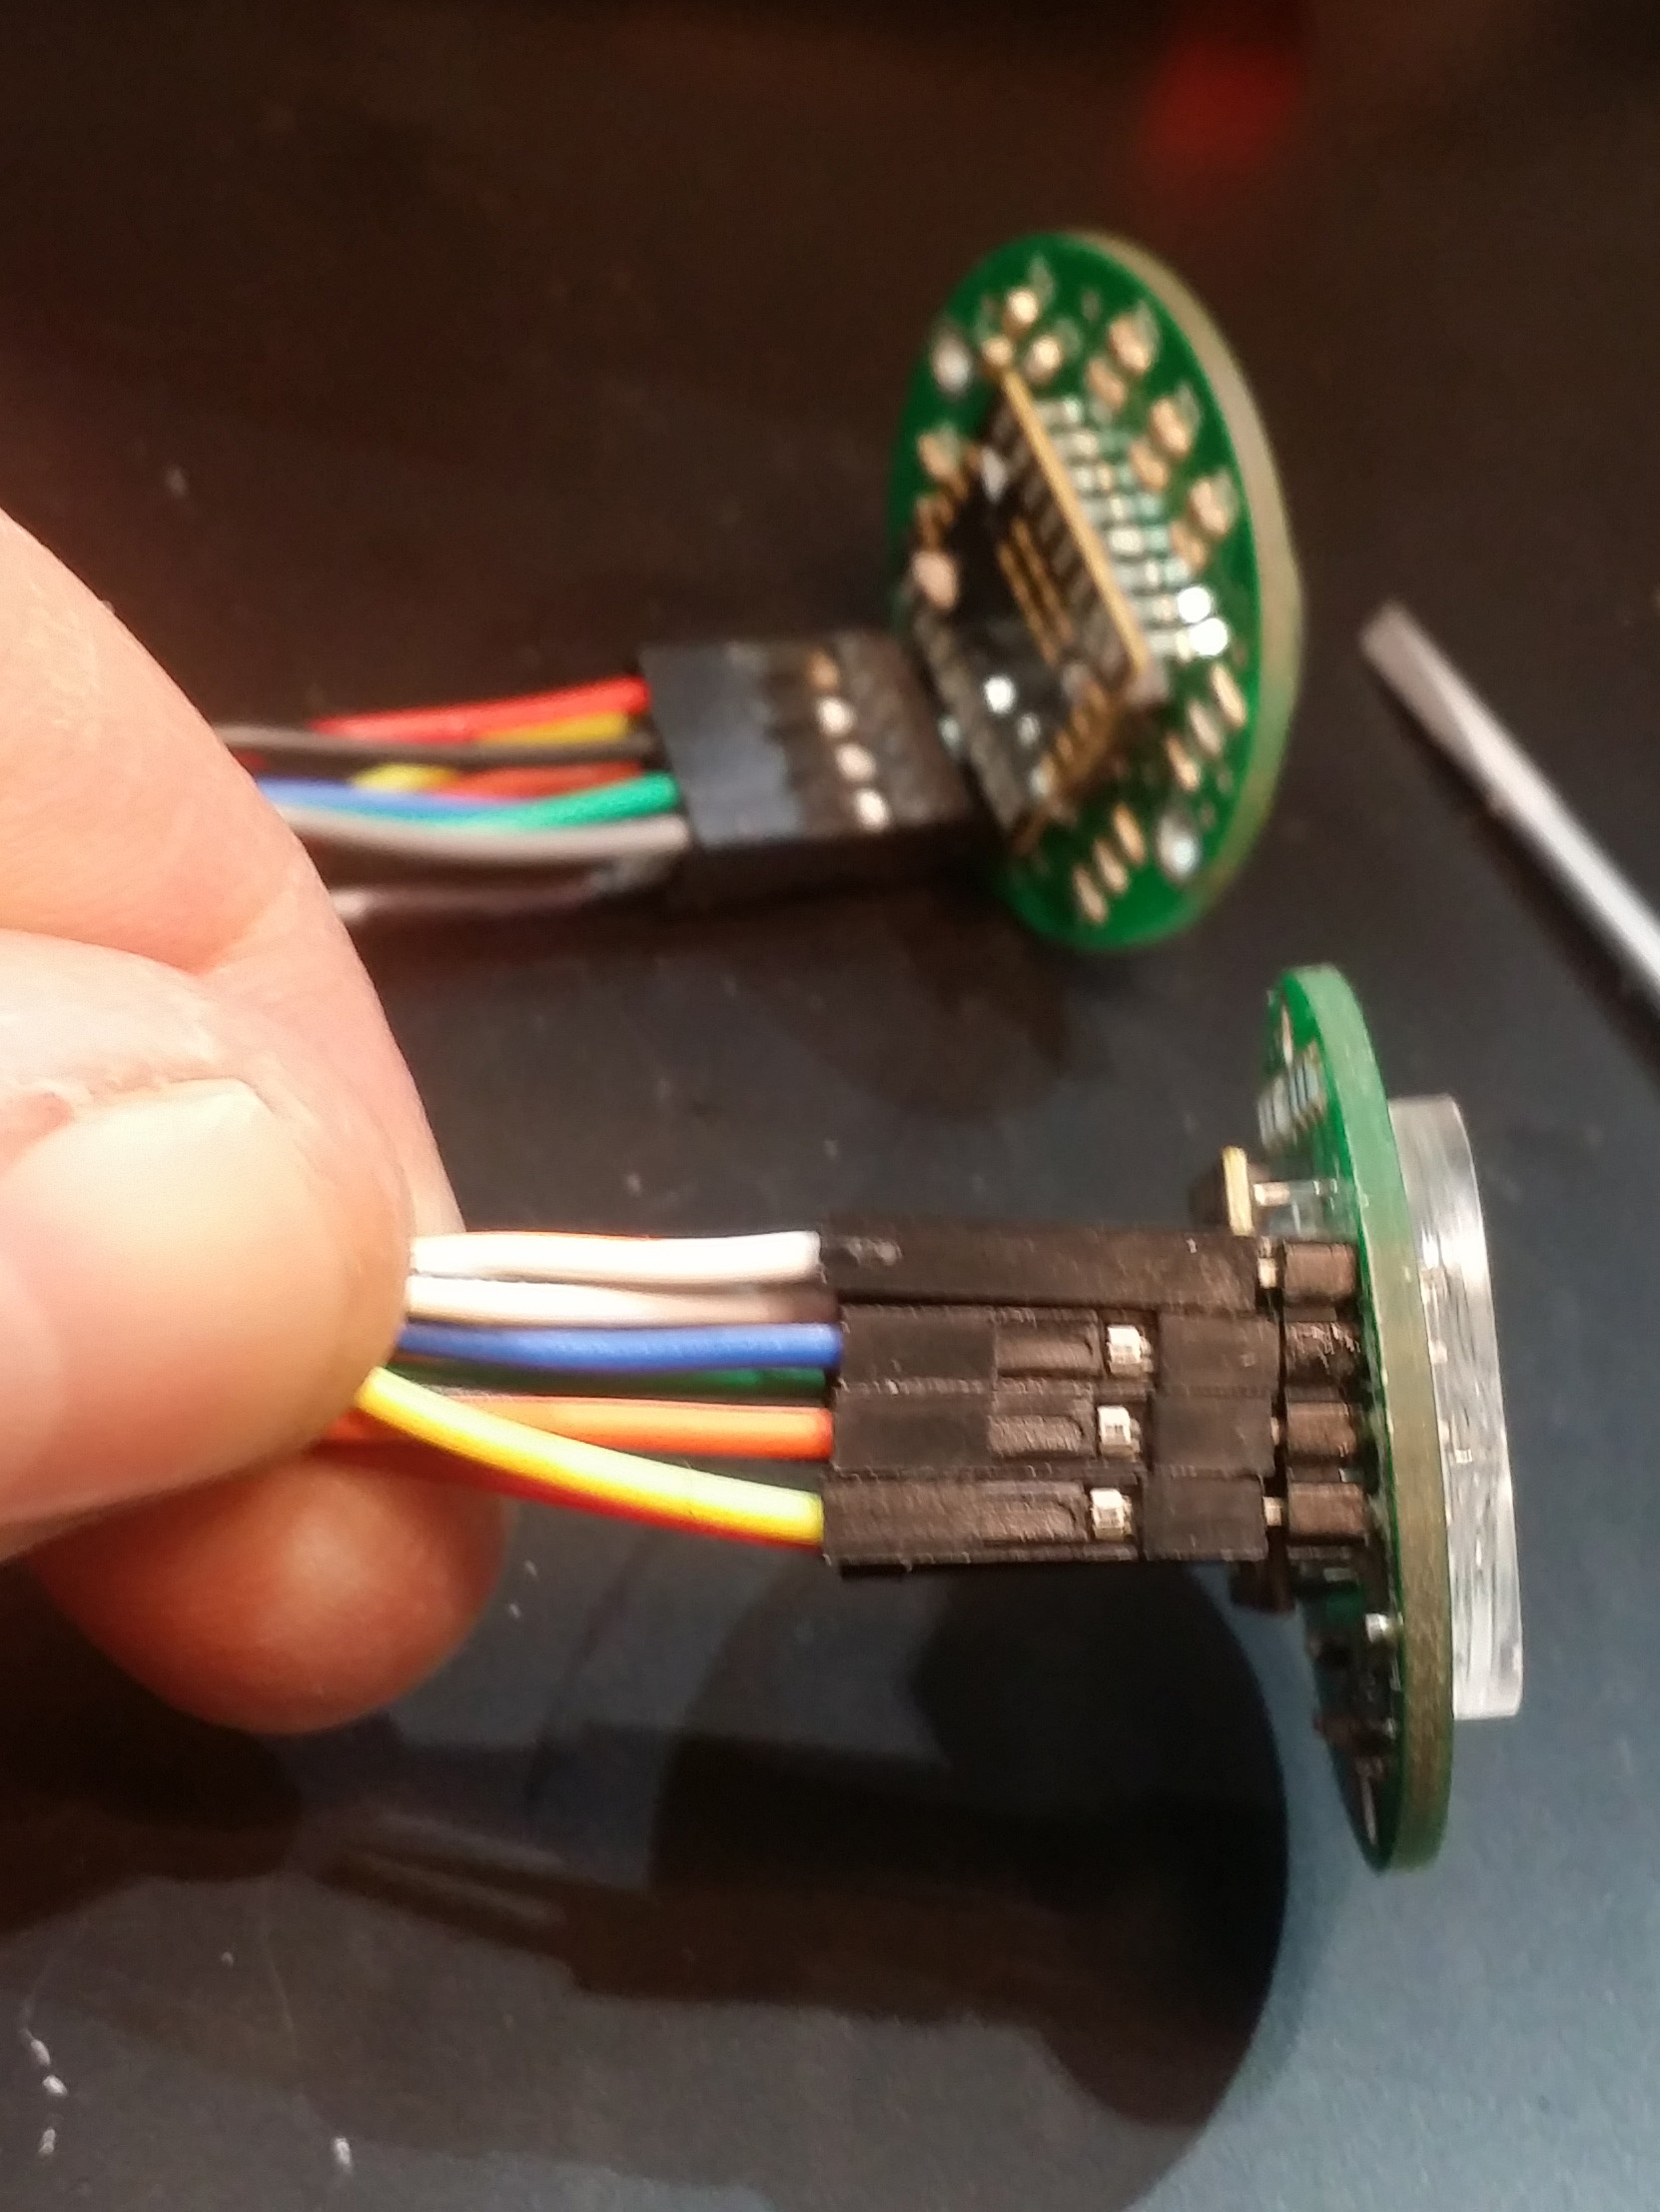
\includegraphics[height=4.5cm]{02-motion-sensors.jpg}
		\centerline{(b)}
	\end{minipage}
	\begin{minipage}[t]{\linewidth}\centering
		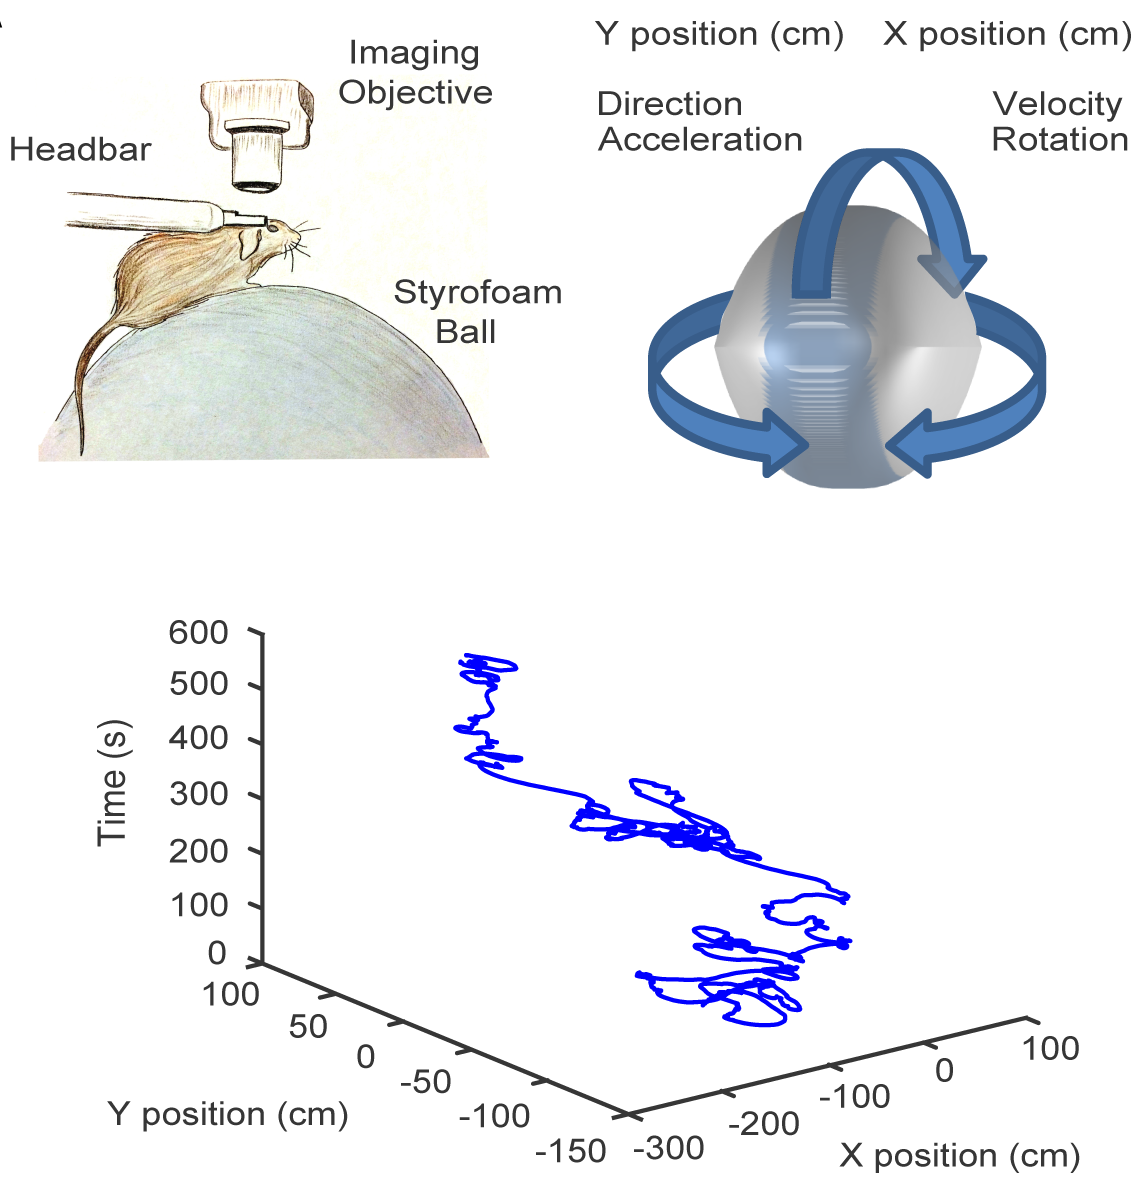
\includegraphics[height=7cm]{striatum_figure2.png}
		\centerline{(c)}
	\end{minipage}
	\caption{
		Motion sensors (a) mention sensors installed;
		(b) motion sensors; (c) tracking mouse movement}
	\label{fig:motion sensors}
\end{figure}

\section{Microscopes}\label{sec:microscopes}

This section describes the background in microscopy in the neurosciences, and also how it relates to imaging in healthcare and electrophysiology in neuroscience.
It will also describe the basic elements necessary for the construction of a microscope in a laboratory where calcium imaging in an animal is available.
It will also refer to later sections which cover the design and construction of mechanical elements for animal handling and optical access (i.e.~the headplate and a chronic optical window).

\subsection{Background: Brain Imaging and Microscopy in Neuroscience}\label{sec:background-brain-imaging-and-microscopy-in-neuroscience}

Optical imaging has traditionally involved wide-field imaging or two photon imaging, each with their own distinctive advantages and disadvantages.
In recent years, two photon microscopy has been a preeminent choice for imaging in tissue, because of its high spatial resolution, and tissue penetrating features.
Two photon calcium imaging has been broadly applied to individual cells or subcellular components of neurons including spines and axons.

Because two photon microscopy uses a scanning mechanism, the signal to noise ratio is influenced by the time spent imaging each point, and the spatial resolution is determined by the number of points scanned to obtain each image.
As a result, the size of the imaging field is inversely correlated with the overall temporal resolution while maintaining a relatively high signal-to-noise ratio, thus, two photon calcium imaging is often performed on a small area or on a sparse network of cells, when dynamic responses with high temporal fidelity is necessary.

Wide-field imaging has been used in various forms for several decades and was first used to characterize the functional architecture and hemodynamic responses in brain tissue.
However, this technique has seen a renaissance recently due to its simple instrumentation, relatively inexpensive cost, and the improvements in neural signal indicators.
Optical imaging and two photon microscopy have traditionally been performed in head-fixed preparations, but recent advances have also made it possible to perform wide-field calcium imaging in freely moving animals, through miniaturized and wearable microendoscope systems

While wide-field imaging lacks the spatial resolution to resolve fine subcellular structure or the penetrating properties available with two-photon, it is possible to obtain clear neurites and somatic features, including spike detection

Because a single photon microscope does not rely on scanning features, it can be used to sample a larger field of view without sacrificing sampling rates.
Additionally, recording sessions may be less sensitive to fluorophore bleaching than other techniques, which makes it possible to perform sustained illumination and subsequent imaging for an extended period of time - a desired feature for analyzing neural networks during some behavior paradigms (e.g., repeated trial learning paradigms).
Thus, wide-field imaging offers an advantage if the objective is to simultaneously recording hundreds of neurons in the brain of a living and behaving animal with high temporal fidelity.

\subsection{Cameras for Widefield Microscopy}\label{sec:cameras-for-widefield-microscopy}

Traditional widefield microscope or macroscope builds incorporate `scientific grade' cameras.
Compared to cameras built for other markets (e.g.~consumer, industrial, studio, etc.)
, these cameras are often well
tested and certified to offer low or well-characterised noise at
moderate speeds, and a linear photo-response profile.
Unlike consumer or studio cameras which are invaribaly configured for RGB color, they are preferably configured with `monochrome' sensors - essentially identical to the analagous color sensor, without the bayer filter.
Of much greater importance, one must consider the unique connectivity and control interface that scientific cameras come with.
Standards exist, but are typically unique to this segment of the industry, with poorly defined specifications for translation to other electronic communication and connection interface standards, such as those used in studio and broadcast video, or those used with consumer cameras.
The trait that is the most worthy of consideration, however, is the cost.
See @discussion-cost-consumer for details.

The in-vivo instrinsic-signal or fluorescent-dye imaging camera of 1 decade ago had a 0.5``-1'' monochrome CCD sensor with 0.1-1 MegaPixels, a large well-depth, and moderately low noise at speeds around 30 to 60 fps.
Connection was often LVDS, with custom electrial connectors unique to each camera.
A particularly popular and long-running model was the Dalsa 1M30, followed by the 1M60 in later years \cite{takahashi_vivo_2006}.

\subsection{Microscope Construction}\label{sec:microscope-construction}

\begin{figure}[htb]
	\begin{minipage}[t]{0.49\linewidth}\centering 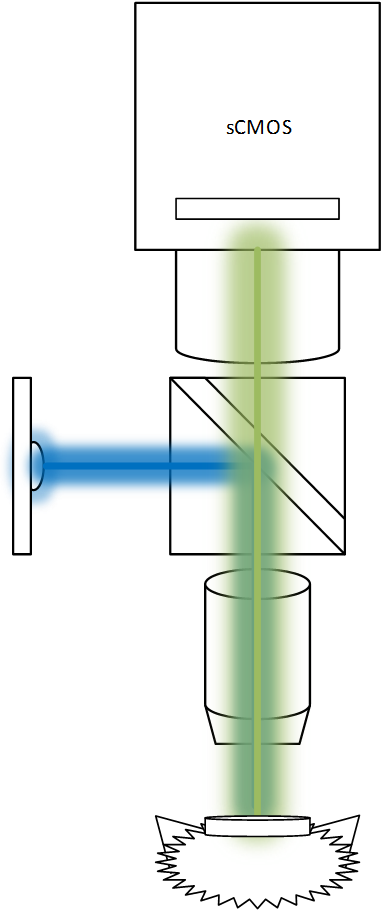
\includegraphics[height=8cm]{widefield_microscope_diagram.png} \medskip \centerline{(a)}
	\end{minipage}
	\hfill
	\begin{minipage}[t]{0.49\linewidth}\centering 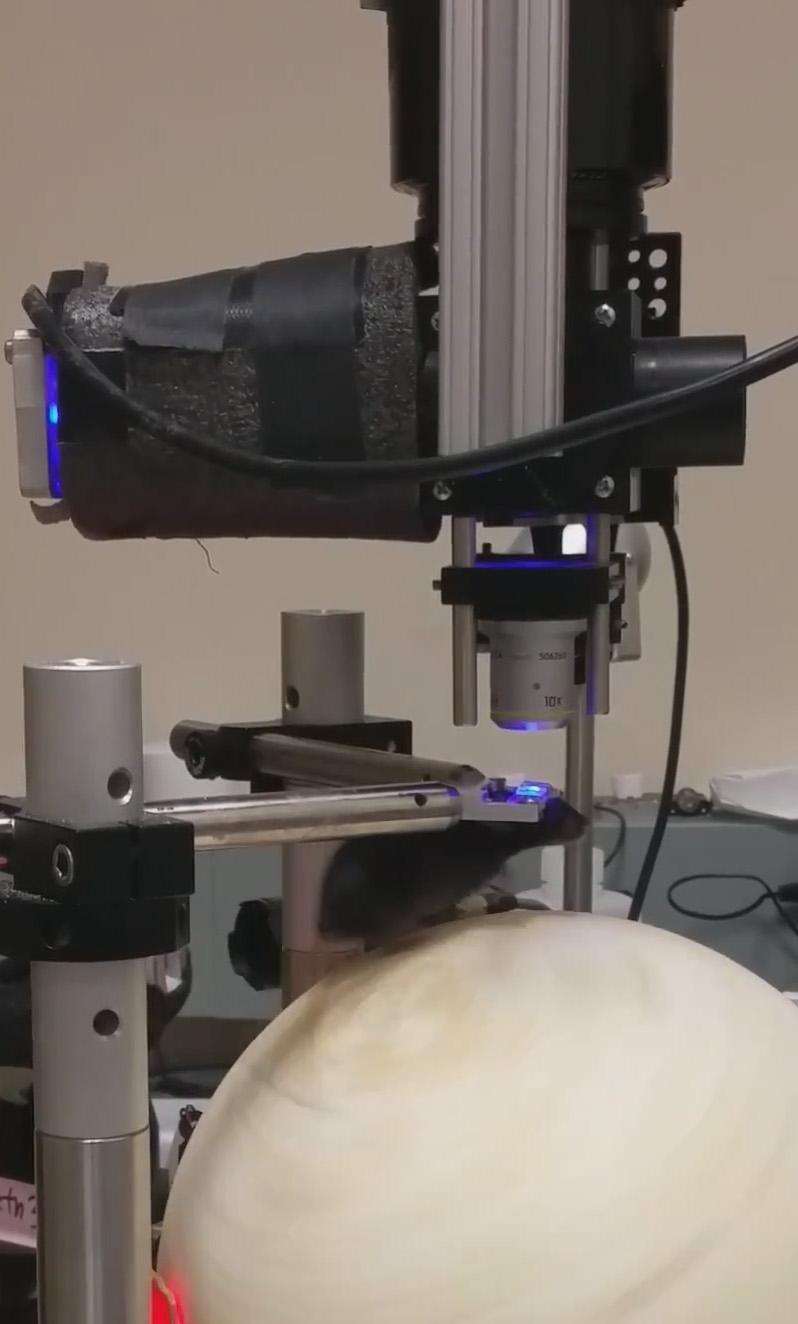
\includegraphics[height=8cm]{setup1.jpg} \medskip \centerline{(b)}
	\end{minipage}
	\caption{Basic configuration for a widefield epifluorescence microscope for in-vivo imaging.
		This first configuration used a phase contrast lens borrowed from an inverted microscope (not recommended).
		(a) Schematic showing relation of microscope and mouse on spherical treadmill; (b) Setup 1: the LED used for extending to the left (black covering to block light)}
	\label{fig:Sampling}
\end{figure}

\begin{figure}[htb]
	\begin{minipage}[t]{0.45\linewidth}\centering
		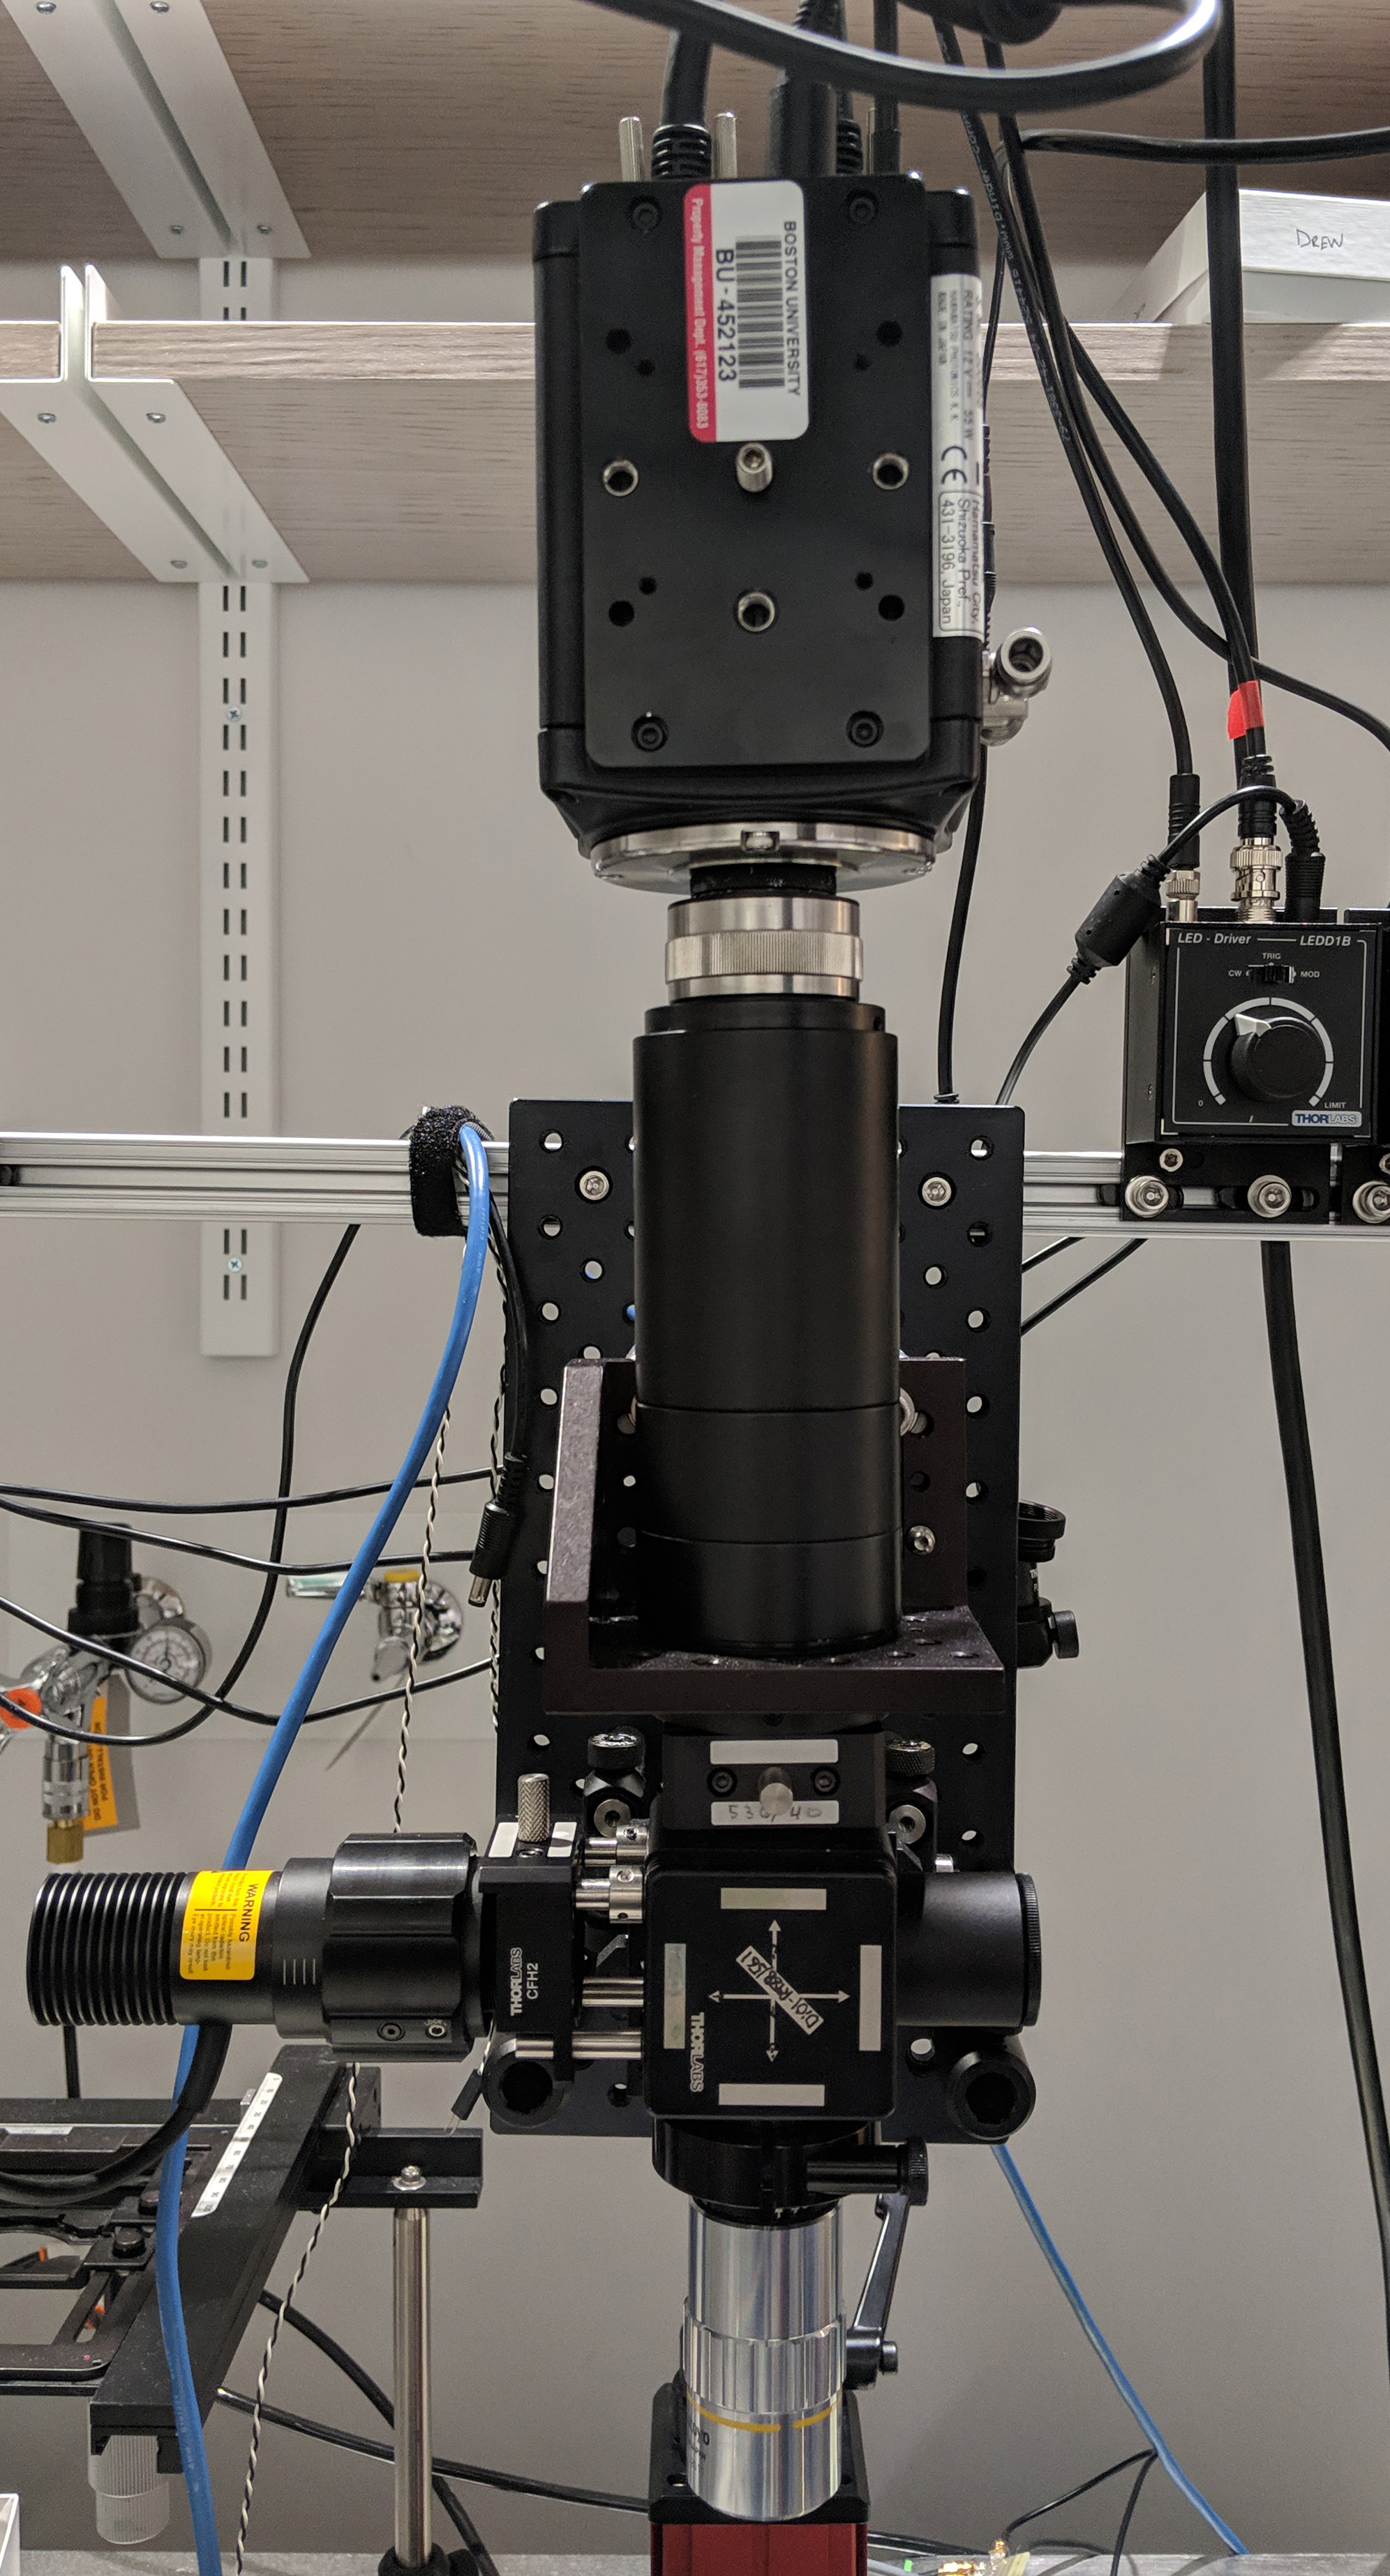
\includegraphics[height=10cm]{setup3-front.jpg}
		\centerline{(a)}
	\end{minipage}
	\hfill
	\begin{minipage}[t]{0.45\linewidth}\centering
		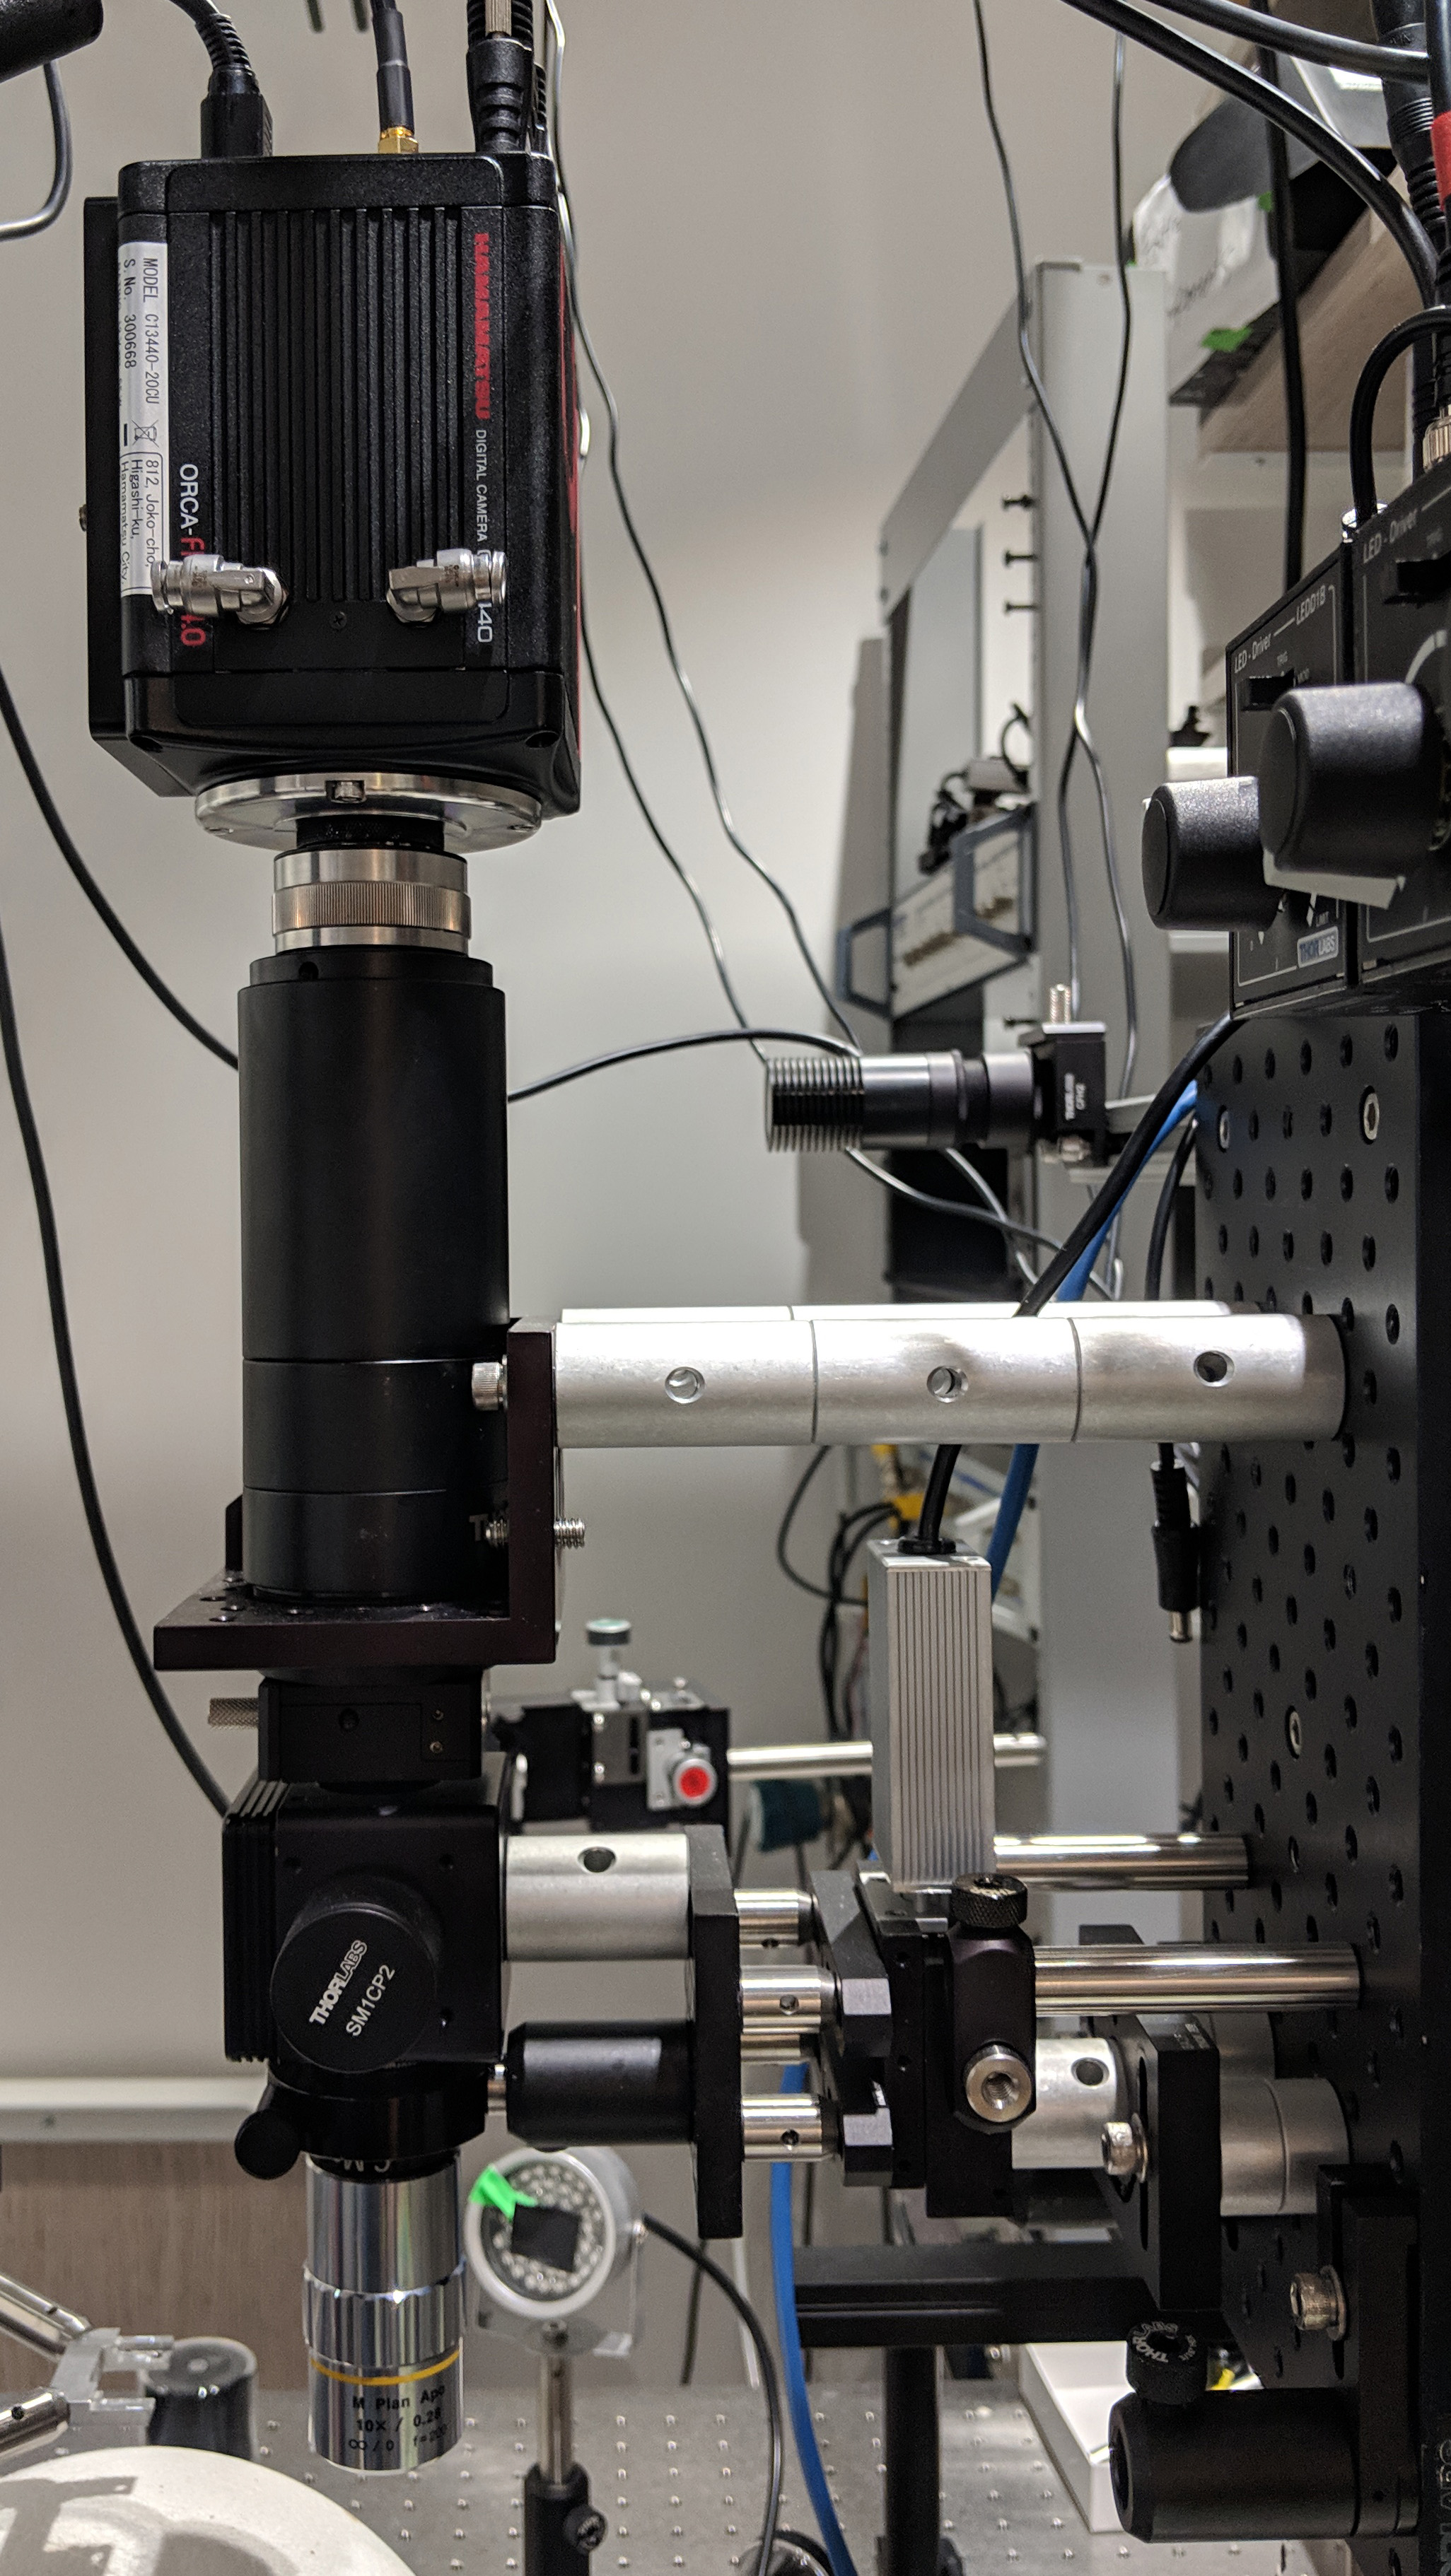
\includegraphics[height=10cm]{setup3-side.jpg}
		\centerline{(b)}
	\end{minipage}
	\begin{minipage}[t]{\linewidth}\centering
		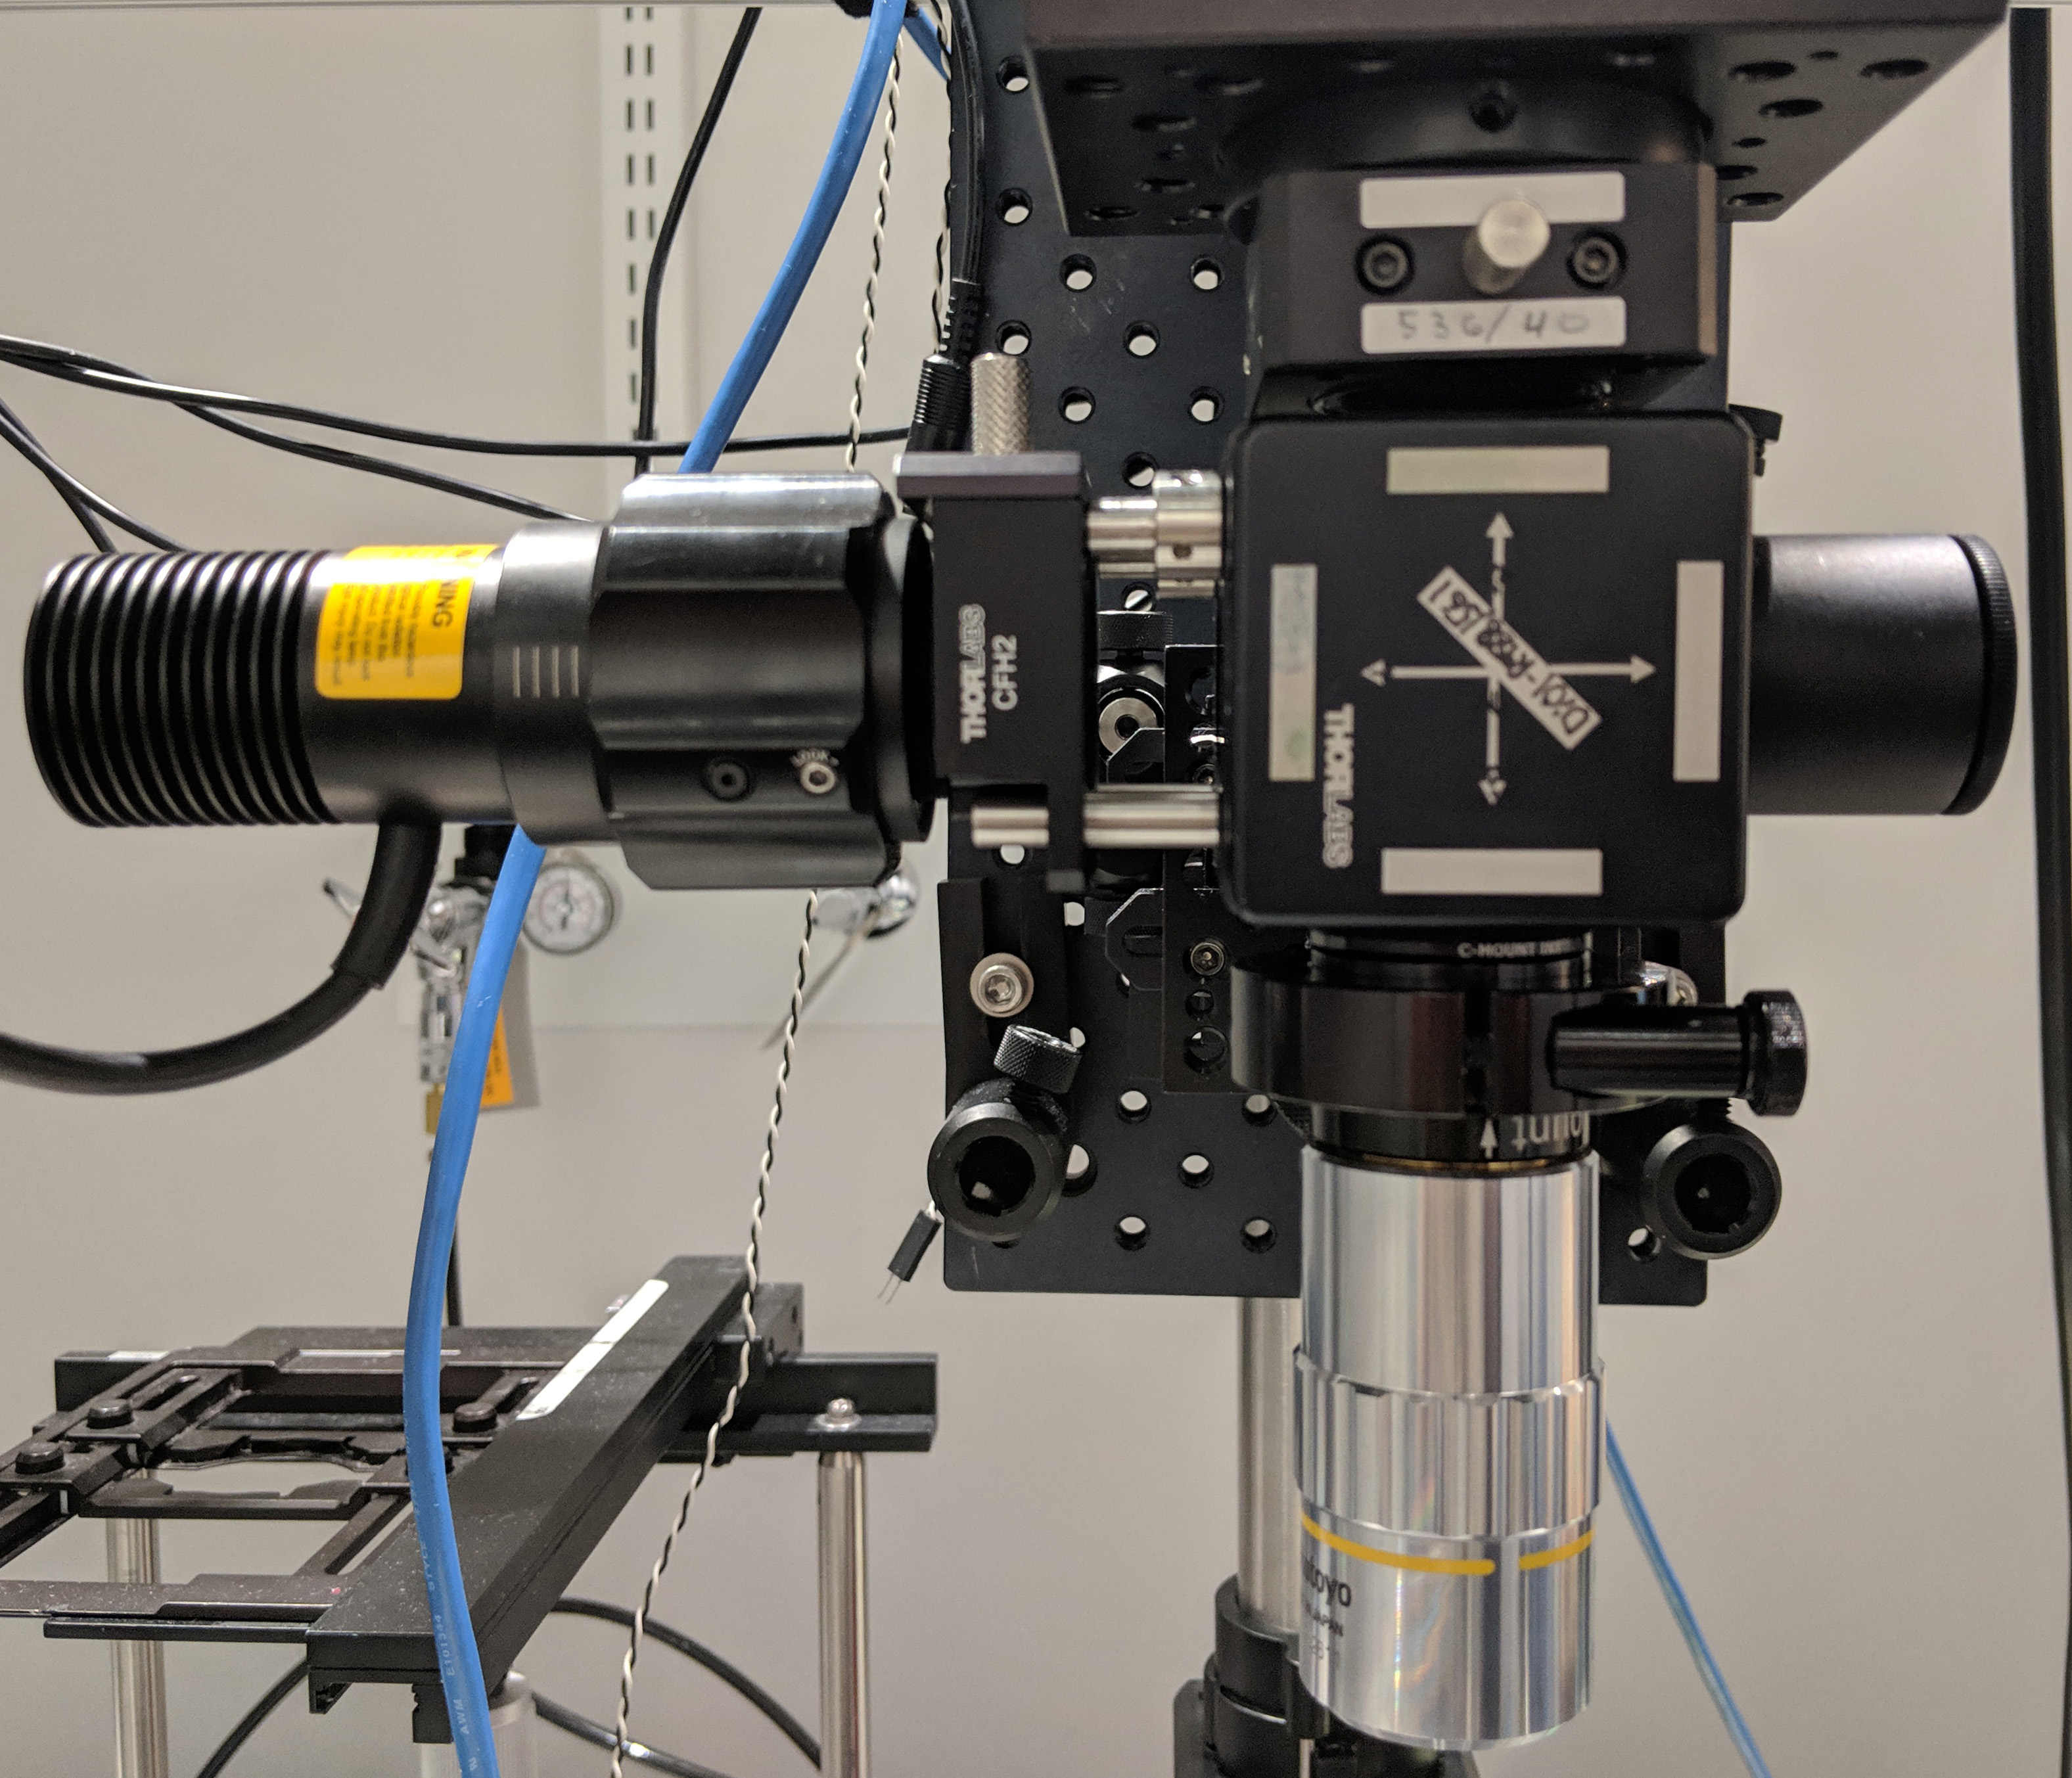
\includegraphics[width=7cm]{setup3-closeup.jpg}
		\centerline{(c)}
	\end{minipage}
	\caption{
		Microscope Setup 2 (a) front;
		(b) close up; (c) side}
	\label{fig:motion sensors}
\end{figure}

\begin{figure}[htb]
	\begin{subfigure}[t]{0.32\textwidth}\centering
		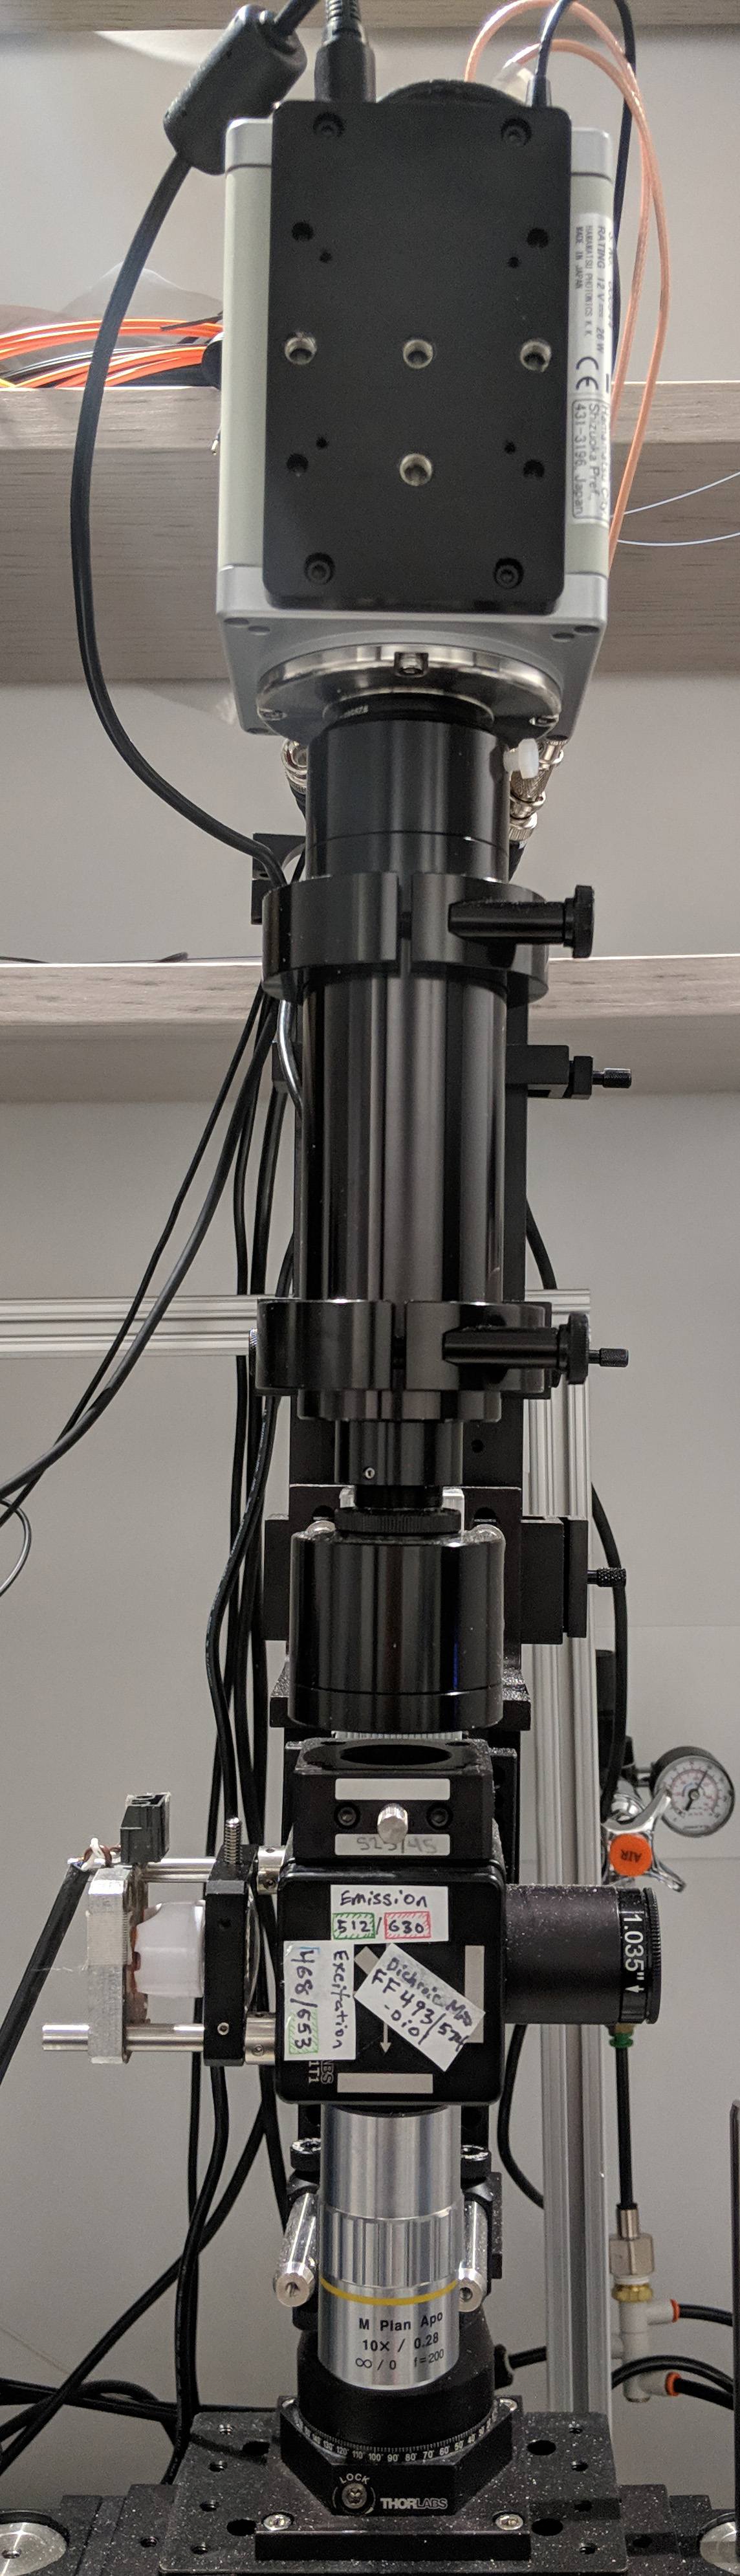
\includegraphics[width=4cm]{setup4-front.jpg}
		% \centerline{(a)}
        \caption{front}
	\end{subfigure}
	\hfill
	\begin{subfigure}[t]{0.32\textwidth}\centering
		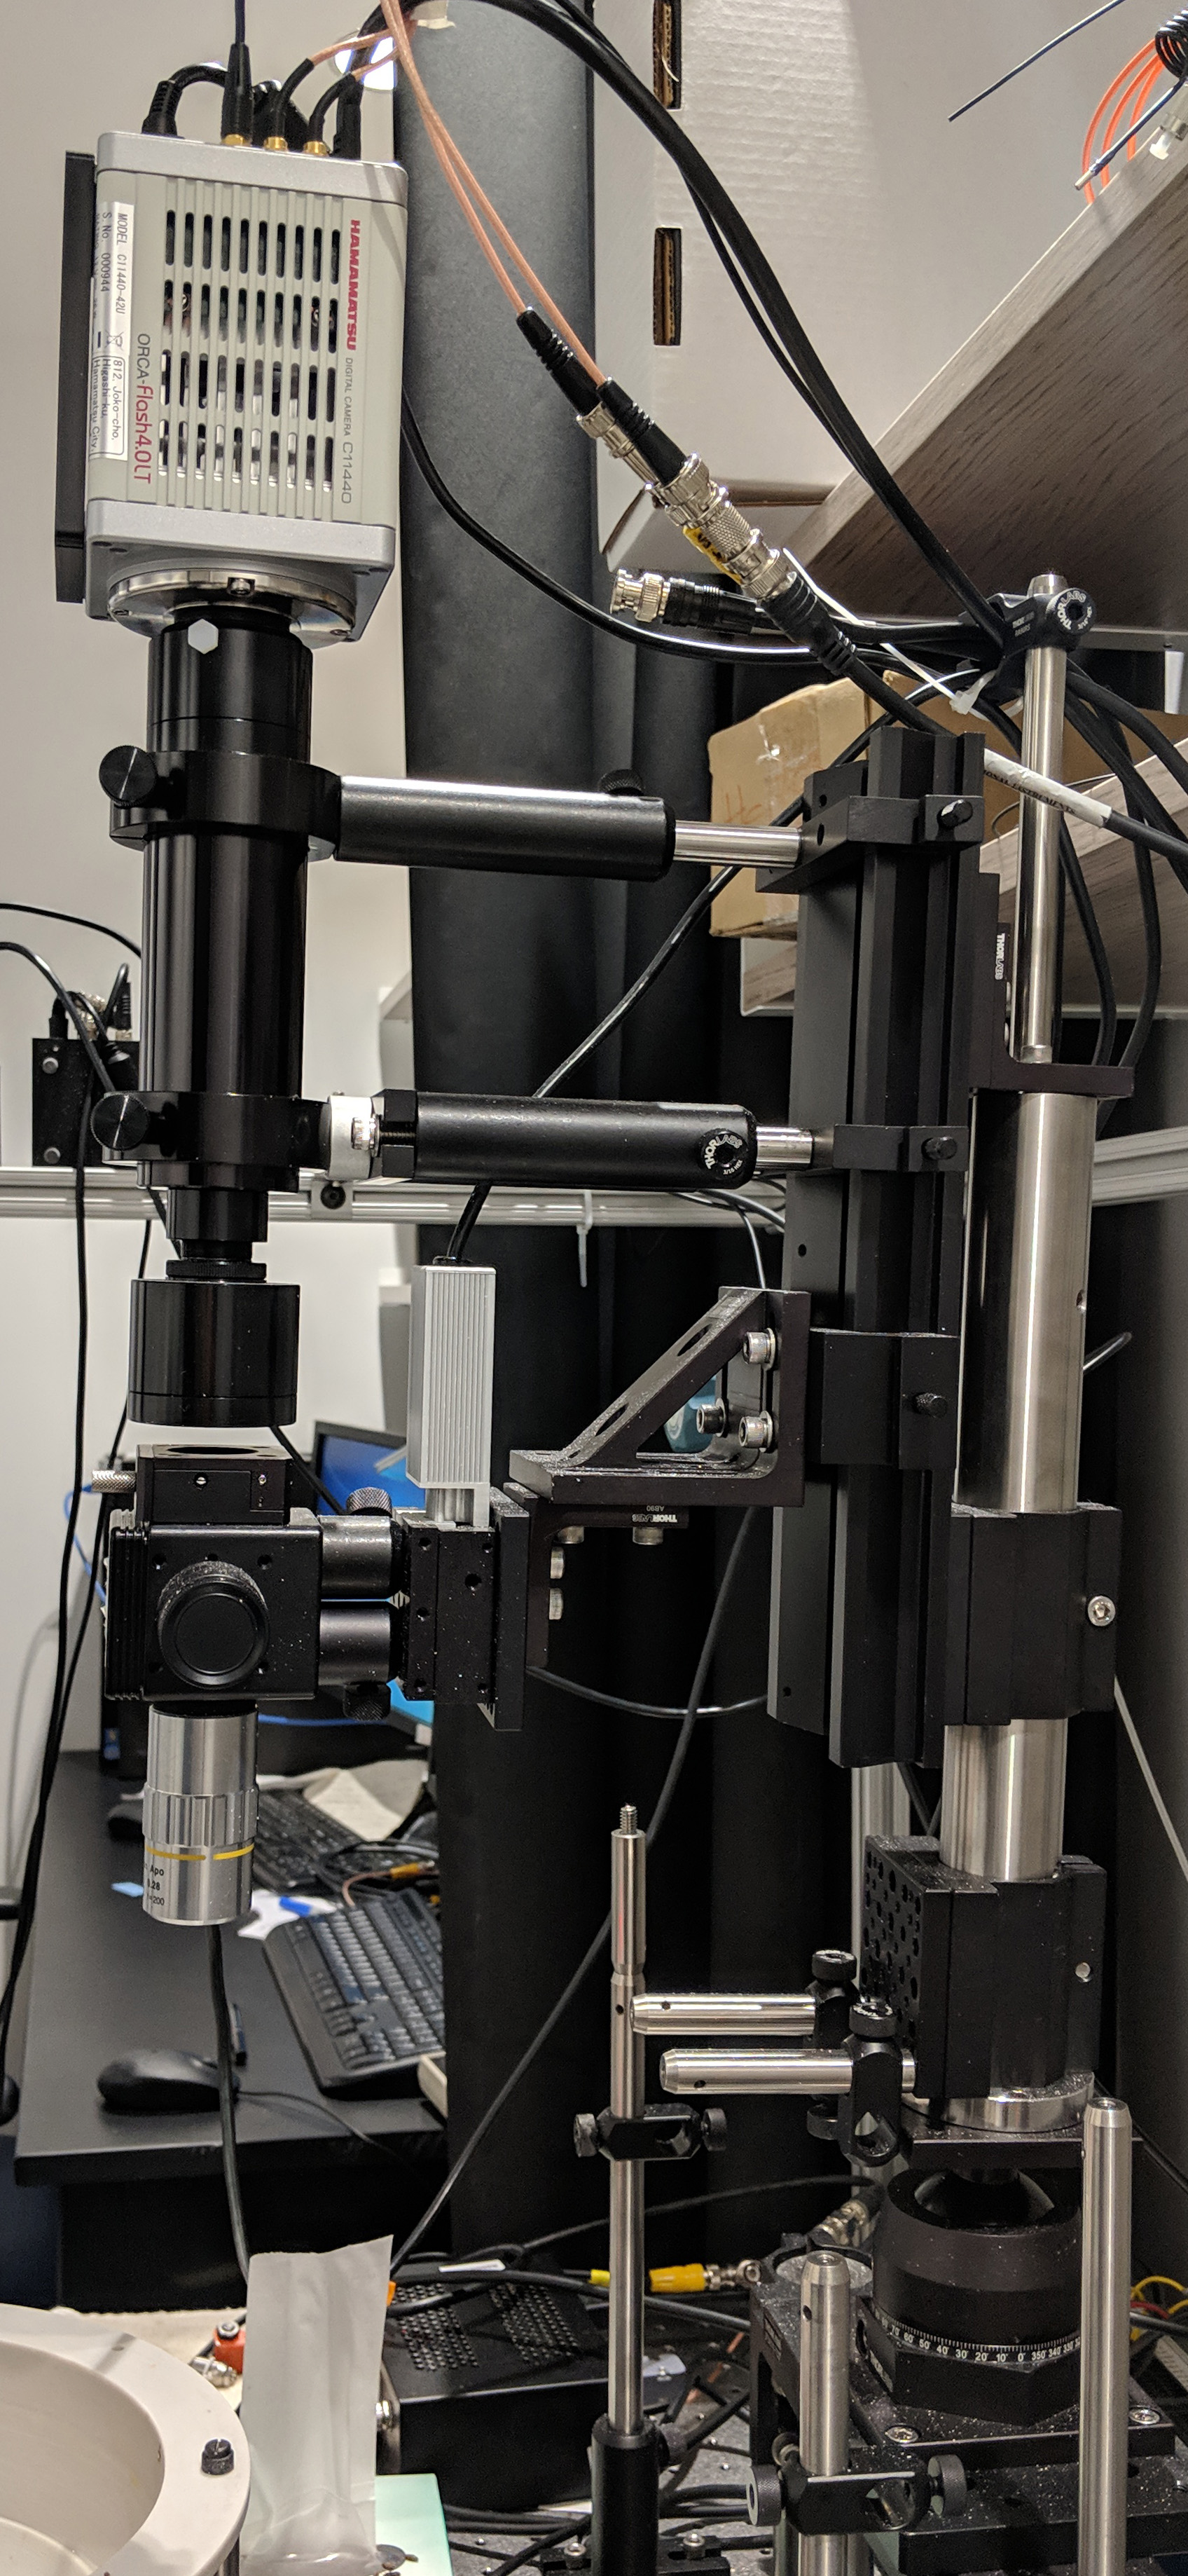
\includegraphics[width=4cm]{setup4-side.jpg}
		% \centerline{(b)}
        \caption{close up}
	\end{subfigure}
	\begin{subfigure}[t]{0.32\textwidth}\centering
		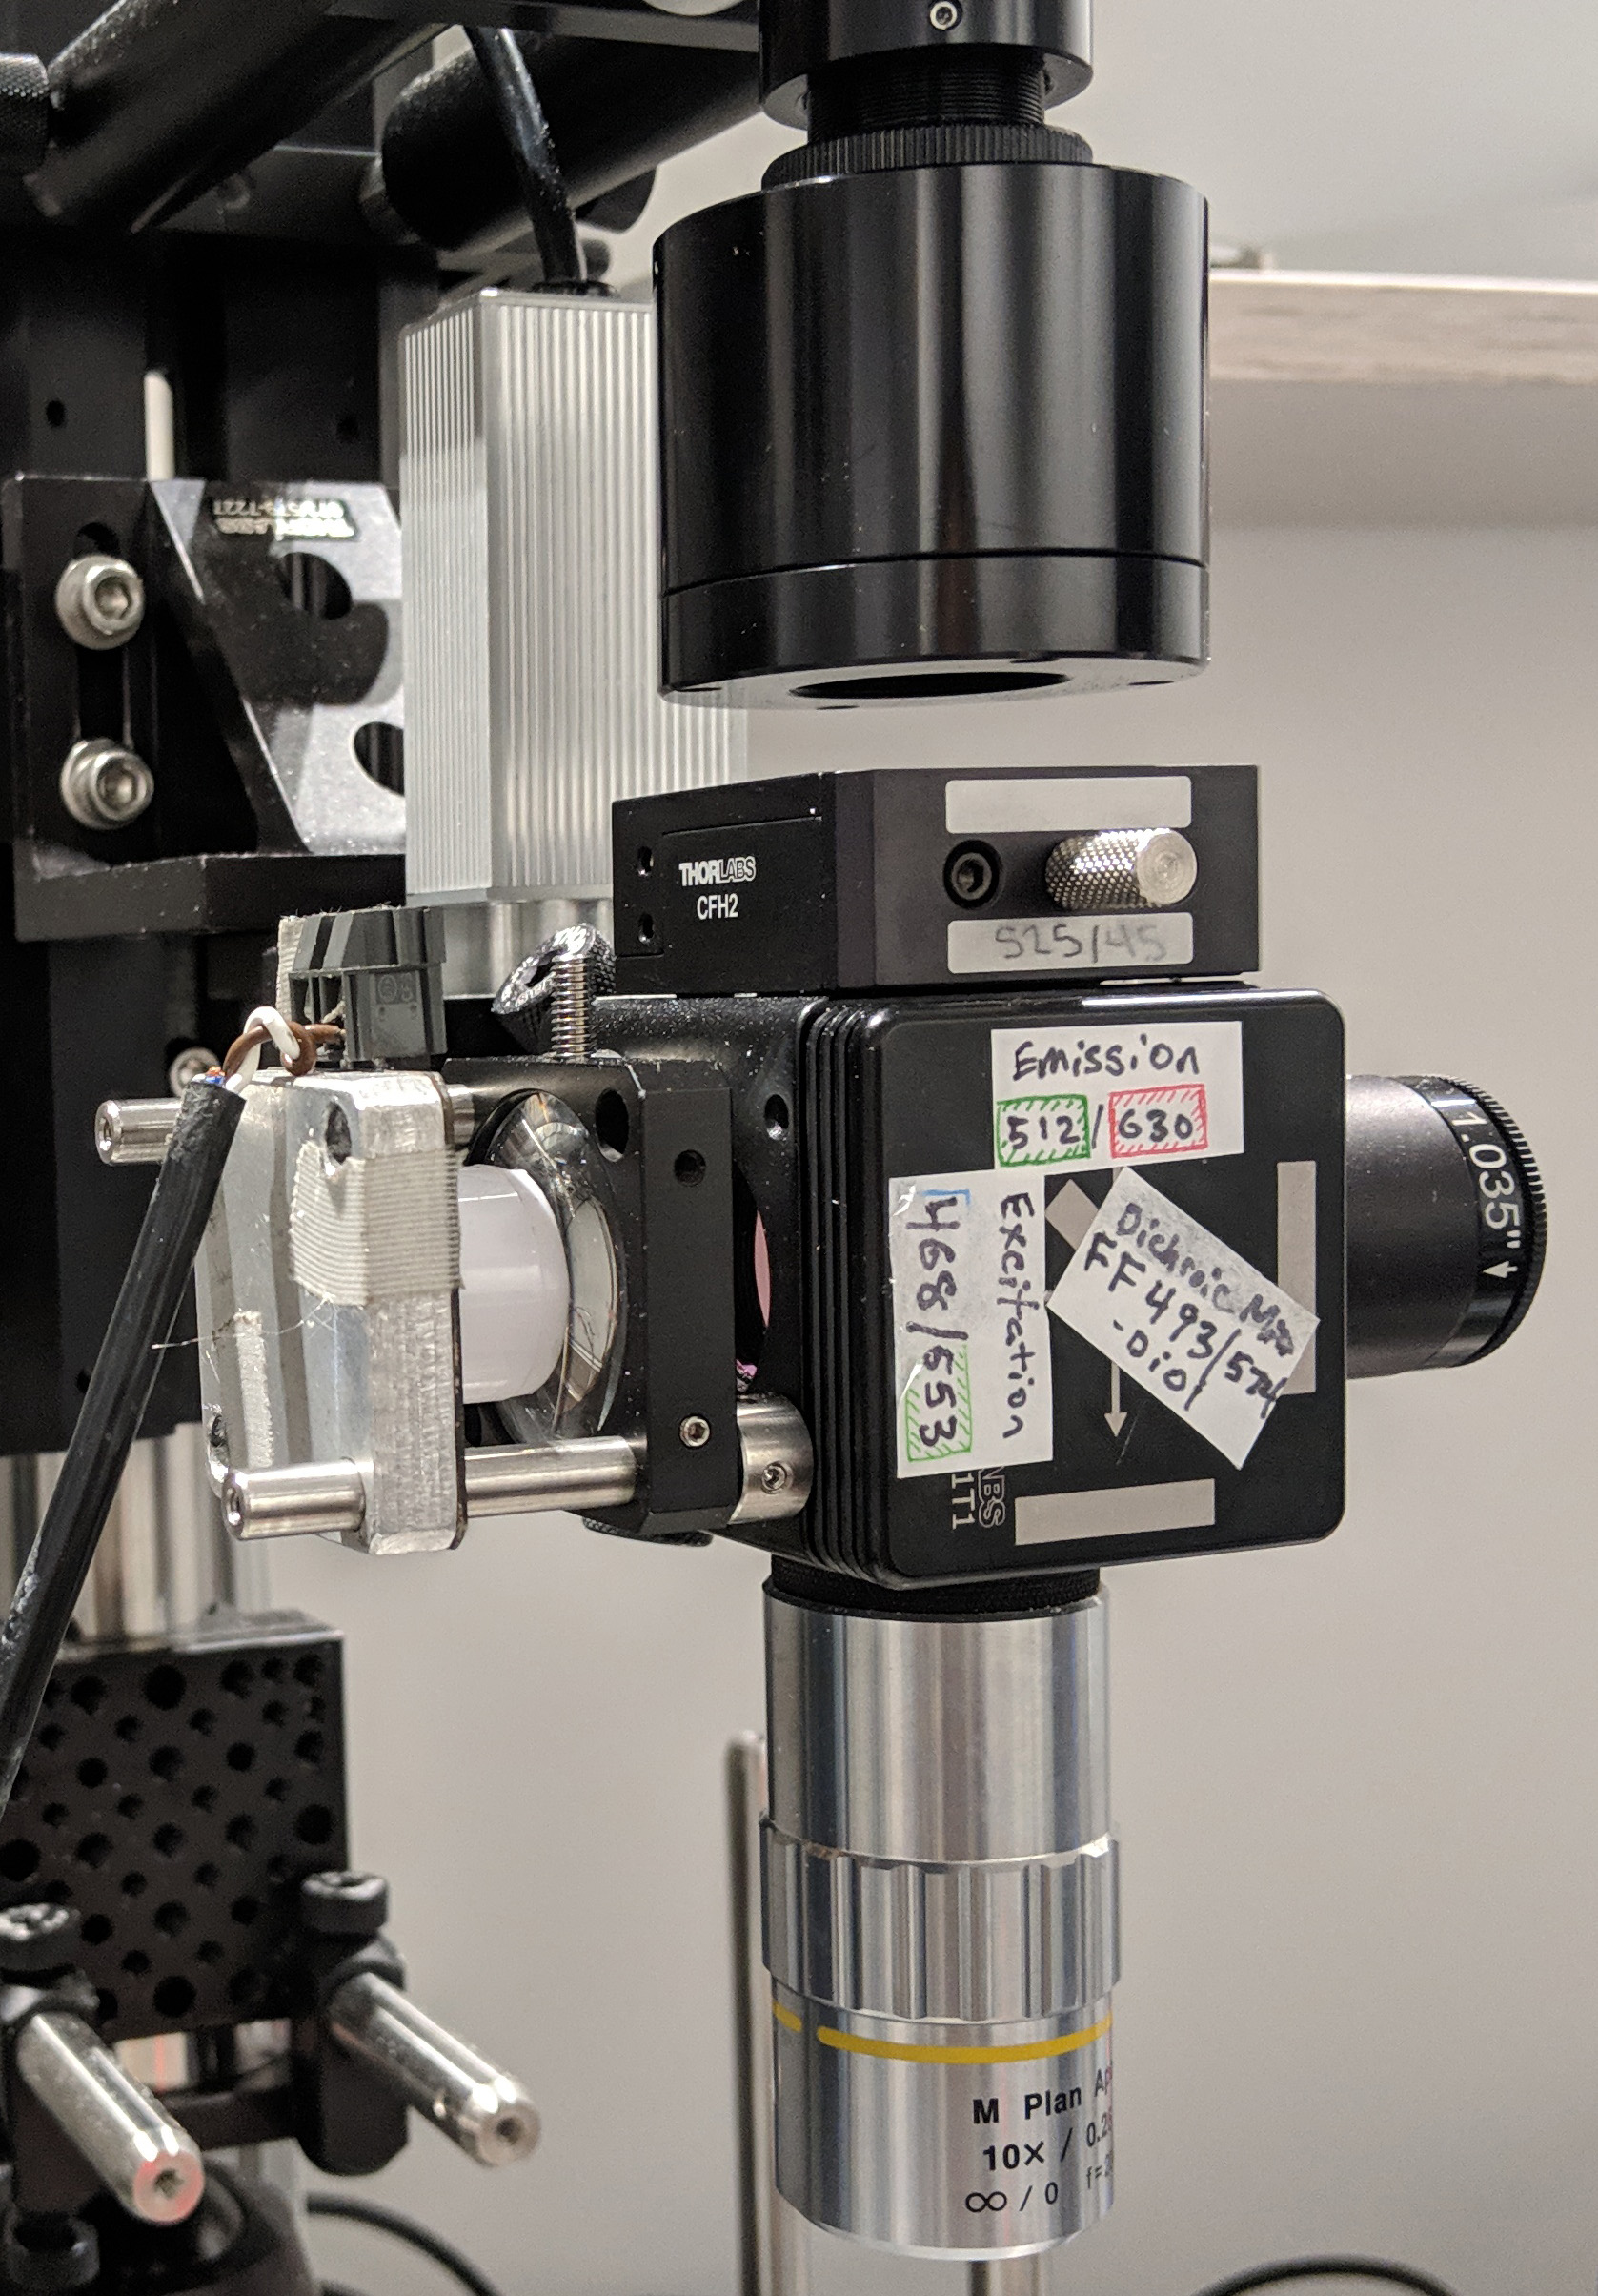
\includegraphics[width=4cm]{setup4-closeup.jpg}
		% \centerline{(c)}
        \caption{side}
	\end{subfigure}
	\caption[Widefield fluorescence microscope reconfigured (Setup 3)]{
		Widefield fluorescence microscope reconfigured Setup 3.
		Multiple iterations are shown, with later iterations offering improved compatibility with usage of off-the-shelf components.}
		% (a) front; (b) close up; (c) side}
	\label{fig:microscope-3}
\end{figure}

%You will also be using a lot of citations. Here is the format required in the dissertation: \cite{lamport1985:latex},\cite{Debr01}.

\clearpage

\end{document}

\cleardoublepage{}


% CHAPTER 3: THE BODY OF THESIS
\documentclass[../main.tex]{subfiles}
\begin{document}

\thispagestyle{myheadings}

\chapter{Neural Signals: Computational considerations, interpretation and usage}
\label{sec:neural-signals}

\section{Image Processing}\label{sec:image-processing}

The entire procedure for processing images and extracting cell signals can be performed in substantially less time than most commonly available tools using the approach described in Aim 1, particularly the methods for restricting the spatial extent of pixel-association operations, and distributing operations across parallel processing cores using a Single Program Multiple Data (SPMD) archetype.
However, the total time still exceeds that of the acquisition session.
Inefficiency arises from the overhead involved with distributing data and passing information between separate parallel processes.
Graphics cards, however execute in what's called Single Instruction Multiple Data (SIMD) fashion, to distribute computation across the thousands of processing cores.

The processing components are implemented using the MATLAB System-Object framework, which allows for slightly faster performance through internal optimizations having to do with memory allocation.
Most system objects, each representing one step in the serial processing and signal-extraction procedure, also have companion functions that implement the computation-heavy components of each algorithm using a pre-compiled CUDA kernel.

\subsection{Benchmarking \& General Performance}\label{sec:benchmarking-general-performance}

Built-in MATLAB functions that execute on the GPU can be profiled with benchmarking functions like \emph{gputimeit()}, or with the \emph{tic/toc} functions.
When execution isn't fast enough, they need to be replaced with custom functions.
The custom functions typically achieve the speed up necessary by enabling the operation to carried out on several frames at once.
This reduces the over-head costs inposed for each function call by spreading it over several frames.
This solution is not ideal, as it increases the latency of solutions, however does not preclude implementation in real-time system if the procedures are adapted to run on a real-time hybrid system-on-module like NVIDIA's Tegra X1, which should involve minimal effort once a standard set of successful procedures is realized.
The current implementation tests the processing time of each stage of the process to ensure that the sum is less than the acquisition time for each frame dictated by the inverse of the frame-rate (30-50 milliseconds).

\subsection{Buffered Operations}\label{sec:buffered-operations}

Combining frames for each operation can result in near linear speedup.
For example, for the phase-correlation step required for motion correction, the FFT and IFFT are called on 16 image-frames at once, and the time take to accomplish is approximately the same as if the operation were called on 1 frame.
This essentially leads to a 16x speedup, though the latency is also increased slightly.
The best size to use is difficult to pre-determine, and typically must be measured for varying size `chunks' using the benchmarking functions indicated above.
The system objects manage the details necessary to allow buffered chunks of video to be passed to each stage without introducing artifacts at the temporal edges between chunks.

\begin{figure}[htb]\centering
	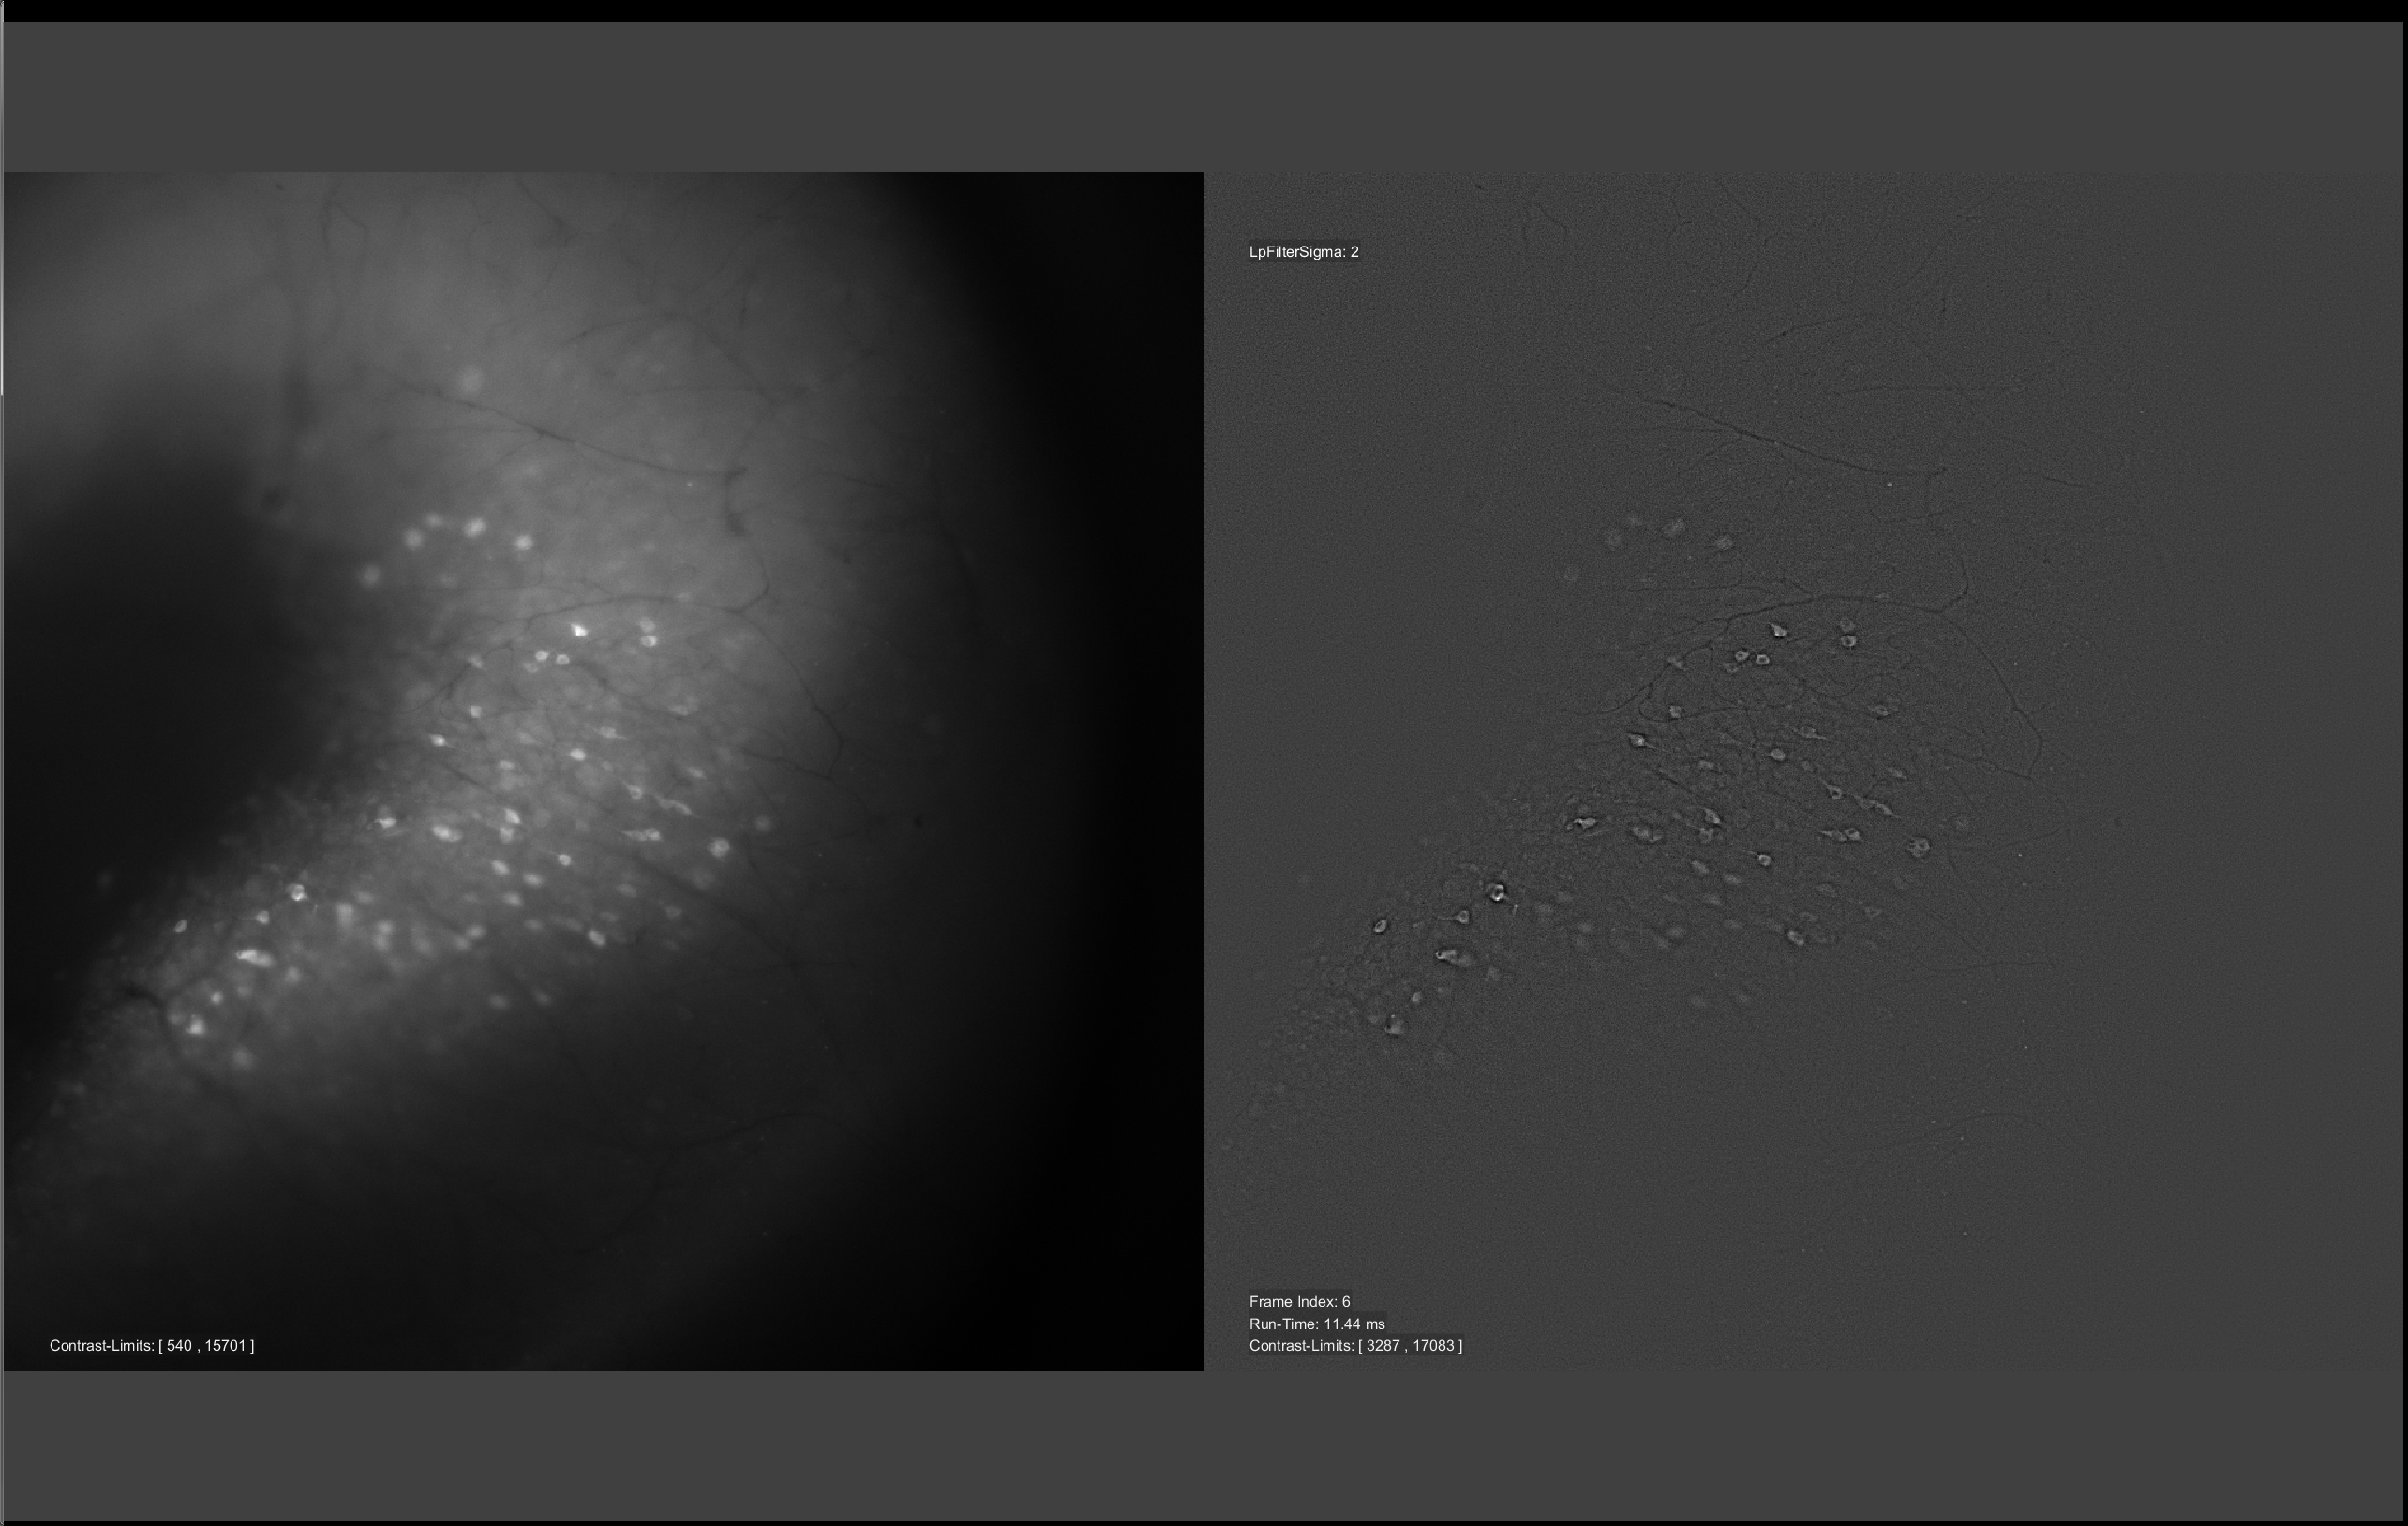
\includegraphics[width=12cm]{screenshot_20150608180058.png}
	\caption{Interactive parameter adjustment for homomorphic filter operation (local contrast enhancement)}
\end{figure}

\subsection{Image Pre-Processing \& Motion Correction}\label{sec:image-pre-processing-motion-correction}

Pre-processing is implemented as with the offline procedure, with a few changes.
Images are aligned in chunks, and they are aligned sequentially to two templates.
One template is the most recent stable frame from the preceding chunk.
The other is a recursively temporal-low-pass filtered image that mitigates slow drifts.
Aligning to the first template is usually more stable as the brightness of cells in the recent image will be more similar to those in the current chunk than will be the brightness of cells in the slow-moving average.

The displacement of each frame is found to sub-pixel precision, then used with a custom bicubic resampling kernel that replaces any pixels at the edges with images from the moving average.



\begin{figure}[htb]\centering
	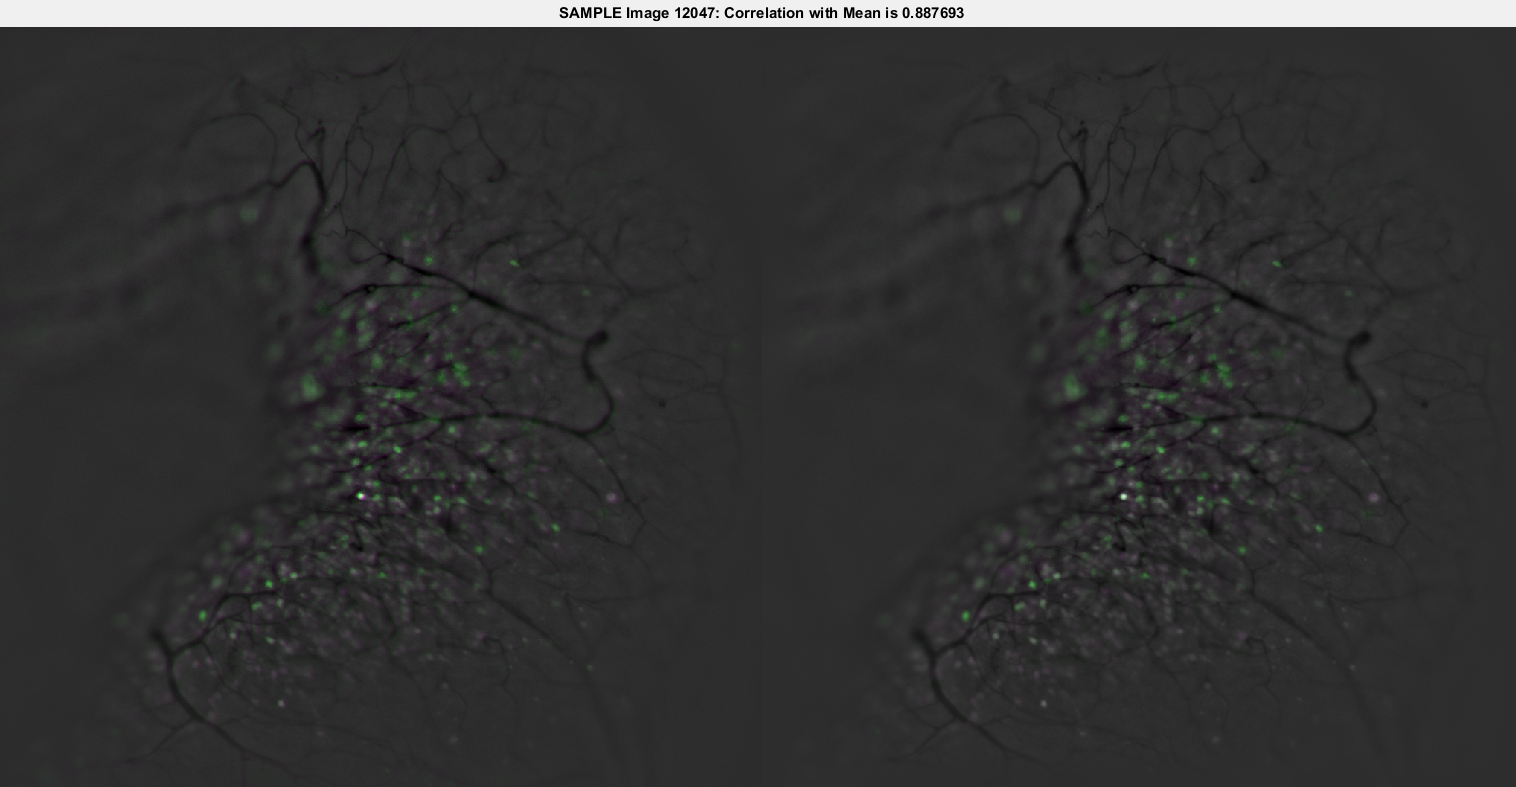
\includegraphics[width=12cm]{motion_correction_sample.png}
	\caption{Motion compensated; comparison of uncompensated and compensated frames overlayed with mean image}
\end{figure}

\subsection{Sequential Statistics}\label{sec:sequential-statistics}

A number of statistics for each pixel are updated online and can be used for normalization and segmentation procedures later in the process.
These include the minimum and maximum pixel intensity, and the first four central moments, which are easily converted to the mean, variance, skewness, and kurtosis.
The formulas for making these calculations are given below, and are performed in a highly efficient manner as data are kept local to each processing core, and repeat computations are minimized.

% \begin{
% 	Shaded} \begin{Highlighting}[] \NormalTok{n = n + }\FloatTok{1}\NormalTok{;
% }
% \NormalTok{f = F(rowIdx,colIdx,k);}
% \NormalTok{d = single(f) - m1;}
% \NormalTok{dk = d/n;}
% \NormalTok{dk2 = dk\textbackslash{}^}\FloatTok{2}\NormalTok{;}
% \NormalTok{s = d\textbackslash{}*dk\textbackslash{}*(n-}\FloatTok{1}\NormalTok{);}

% \CommentTok{% UPDATE CENTRAL MOMENTS}
% \NormalTok{m1 = m1 + dk;}
% \NormalTok{m4 = m4 + s\textbackslash{}*dk2\textbackslash{}*(n.\textbackslash{}^}\FloatTok{2}\NormalTok{-}\FloatTok{3}\NormalTok{\textbackslash{}*n+}\FloatTok{3}\NormalTok{) + }\FloatTok{6}\NormalTok{\textbackslash{}*dk2\textbackslash{}*m2 - }\FloatTok{4}\NormalTok{\textbackslash{}*dk\textbackslash{}*m3;}
% \NormalTok{m3 = m3 + s\textbackslash{}*dk\textbackslash{}*(n-}\FloatTok{2}\NormalTok{) - }\FloatTok{3}\NormalTok{\textbackslash{}*dk\textbackslash{}*m2;}
% \NormalTok{m2 = m2 + s;}

% \CommentTok{% UPDATE MIN & MAX}
% \NormalTok{fmin = min(fmin, f);}
% \NormalTok{fmax = max(fmax, f);}
% \end{
% 	Highlighting} \end{Shaded}

Furthermore, the value used to update each central moment at each point in time can be used as a measure of change in the distribution of each pixel caused by the current pixel intensity, as explained next.

\subsubsection{Non-Stationarity \& Differential Moments}\label{sec:non-stationarity-differential-moments}

Stationary refers to the property of a signal such that its statistics do not vary over time, i.e.~its distribution is stable.
Neural signals tend to specifically \emph{not} have this property, in contrast to other measurable components such as those contributed by physiologic noise (heart-rate, respirations, etc.)
.
Thus, by analyzing the evolution of statistical measures calculated for each pixel as frames are added in sequence gives a highly sensitive indicator of neural activity.
This is done using a routine analogous to that for updating central moments given above, except the values returned are not only the updated moment, but also the updating component -- essentially the partial derivative with respect to time.
This is illustrated below, including the normalization functions which convert the partial-moment values to their variance, skewness, and kurtosis analogues:

% \begin{Shaded} \begin{Highlighting}[] \NormalTok{dm1 = dk;
% }
% \NormalTok{m1 = m1 + dm1;}
% \NormalTok{dm4 = s\textbackslash{}*dk2\textbackslash{}*(n\textbackslash{}^}\FloatTok{2}\NormalTok{-}\FloatTok{3}\NormalTok{\textbackslash{}*n+}\FloatTok{3}\NormalTok{) + }\FloatTok{6}\NormalTok{\textbackslash{}*dk2\textbackslash{}*m2 - }\FloatTok{4}\NormalTok{\textbackslash{}*dk\textbackslash{}*m3;}
% \NormalTok{dm3 = s\textbackslash{}*dk\textbackslash{}*(n-}\FloatTok{2}\NormalTok{) - }\FloatTok{3}\NormalTok{\textbackslash{}*dk\textbackslash{}*m2;}
% \NormalTok{dm2 = s;}
% \NormalTok{m2 = m2 + dm2;}
% \NormalTok{dm2 = dm2/max(}\FloatTok{1}\NormalTok{,n-}\FloatTok{1}\NormalTok{);}
% \NormalTok{dm3 = dm3\textbackslash{}*sqrt(max(}\FloatTok{1}\NormalTok{,n))/(m2\textbackslash{}^}\FloatTok{1.5}\NormalTok{);}
% \NormalTok{dm4 = dm4\textbackslash{}*n/(m2\textbackslash{}^}\FloatTok{2}\NormalTok{);}
% \end{
% 	Highlighting} \end{Shaded}

% Caption: Differential-update-to-central-moments

These functions run on images representing the image intensity, and also on images taken from sequential differences indicating the temporal derivative of image intensity.
The combination of outputs from these operations indicate both when image intensities are significantly high relative to past distribution, and also when intensities are changing significantly faster than learned from their past distribution.

\begin{listing}[ht]
\inputminted[
frame=lines,
framesep=2mm,
bgcolor=black,
baselinestretch=1.0,
fontsize=10pt
]
{matlab}{updateStatisticStructure.m}
\caption{Incremental update of the statistics structure (min, max, and first 4 central moments)}
\label{listing:update-statistic}
\end{listing}

This type of function is also easily trasnalted to stencil functions on for computation on the GPU.

% \begin{listing}[ht]
% \inputminted[
% frame=lines,
% framesep=2mm,
% bgcolor=black,
% baselinestretch=1.0,
% fontsize=10pt
% ]
% {matlab}{updateStatisticsGPU.m}
% \caption{Incremental update of the statistics structure programmed to run as pixel-wise CUDA kernel on GPU}
% \label{listing:update-statistic-gpu}
% \end{listing}

\begin{listing}[ht]
\begin{minted}{matlab}
function [fmin,fmax,m1,m2,m3,m4,n] = statUpdateKernel(f,fmin,fmax,m1,m2,m3,m4,n)

    % update sample count for this pixel
    n = n + 1;

    % precompute & cache some values for speed
    d = f - m1;
    dk = d/n;
    dk2 = dk^2;
    s = d*dk*(n-1);

    % update central moments
    m1 = m1 + dk;
    m4 = m4 + s*dk2*(n.^2-3*n+3) + 6*dk2*m2 - 4*dk*m3;
    m3 = m3 + s*dk*(n-2) - 3*dk*m2;
    m2 = m2 + s;

    % update min & max
    fmin = min(fmin, f);
    fmax = max(fmax, f);

end
\end{minted}
\caption{Incremental update of the statistics structure programmed to run as pixel-wise CUDA kernel on GPU}
\label{listing:update-statistic-gpu}
\end{listing}

\subsection{Surface Classification: Peaks, Edges, Curvature}\label{sec:surface-classification-peaks-edges-curvature}

Edge-finding methods are employed for establishing boundaries between cells, and first and second-order gradients are used to compute local measures of curvature from an eigenvalue decomposition of the local Hessian matrix.
I won't go into detail, as the utility of these procedure in the most recent implementation has been lost, but nevertheless, the operation is optimized and ready to be plugged back in when further development calls for better accuracy informing cell-segmentation, or when a faster or more accurate motion-correction algorithm is called for.

\subsection{Online Cell Segmentation \& Tracking}\label{sec:online-cell-segmentation-tracking}

Cells are segmented by first running sequential statistics on the properties of identifiable regions on a pixel-wise basis.
That is, as regions are identified in a method similar to that used offline in Aim 1, the region-properties are calculated (Centroid, Bounding-Box, etc.) and statistics for these properties are updated at each pixel covered by a proposed region.
After sufficient evidence has gathered, Seeds are generated by finding the local peak of a seed-probability function that optimizes each pixel's proximity to a region centroid, and distance from any boundary.
Regions are grown from these seed regions, and registered in a hierarchy that allows for co-labeling of cellular and sub-cellular components.
Newly identified regions occur as new seeds, where as seeds overlapping with old regions are used to identify sub-regions, or to track regions over time.

\subsection{Signal Extraction from Subcellular Compartments}\label{sec:signal-extraction-from-subcellular-compartments}

I also have functions for the extraction of normalized Pointwise-Mutual-Information (nPMI), which can operate on a pixel-to-pixel basis or on a region-to-pixel basis.
This operation accumulates mutually informative changes in all pixels in the maximal bounding-box (e.g.~64x64 pixels) surrounding each identified regions centroid.
The weights given by this function can take on values between -1 and 1, and can be used to inform any reduction operations to follow.
Additionally, spatial moments can indicate the subcellular distribution of activity across the identified region.
In this context, the first spatial moment M\textsubscript{00} indicates the mean signal intensity.

\begin{listing}[ht]
\inputminted[
frame=lines,
framesep=2mm,
bgcolor=black,
baselinestretch=1.0,
fontsize=10pt
]
{matlab}{pointwiseMutualInformationRunGpuKernel.m}
\caption{Incremental update of point-wise normalized mutual information, assessed in the local neighborhood of each pixel}
\label{listing:npmi}
\end{listing}

\subsection{User Interface for Parameter Tuning}\label{sec:user-interface-for-parameter-tuning}

Some system-objects also incorporate a user interface to aid in parameter selection for tuning.

\subsection{Image Processing: Tone mapping and Filtering}\label{sec:image-processing-tonemapping-and-filtering}
\begin{figure}[htb]\centering
	\includegraphics[height=12cm]{sw-video-processing-feature-generation.png}
	\caption{Feature generation showing complex-valued moving average of distance of each pixel to bounding box corners (post segmentation)}
\end{figure}

% \begin{figure}[htb]\centering
% 	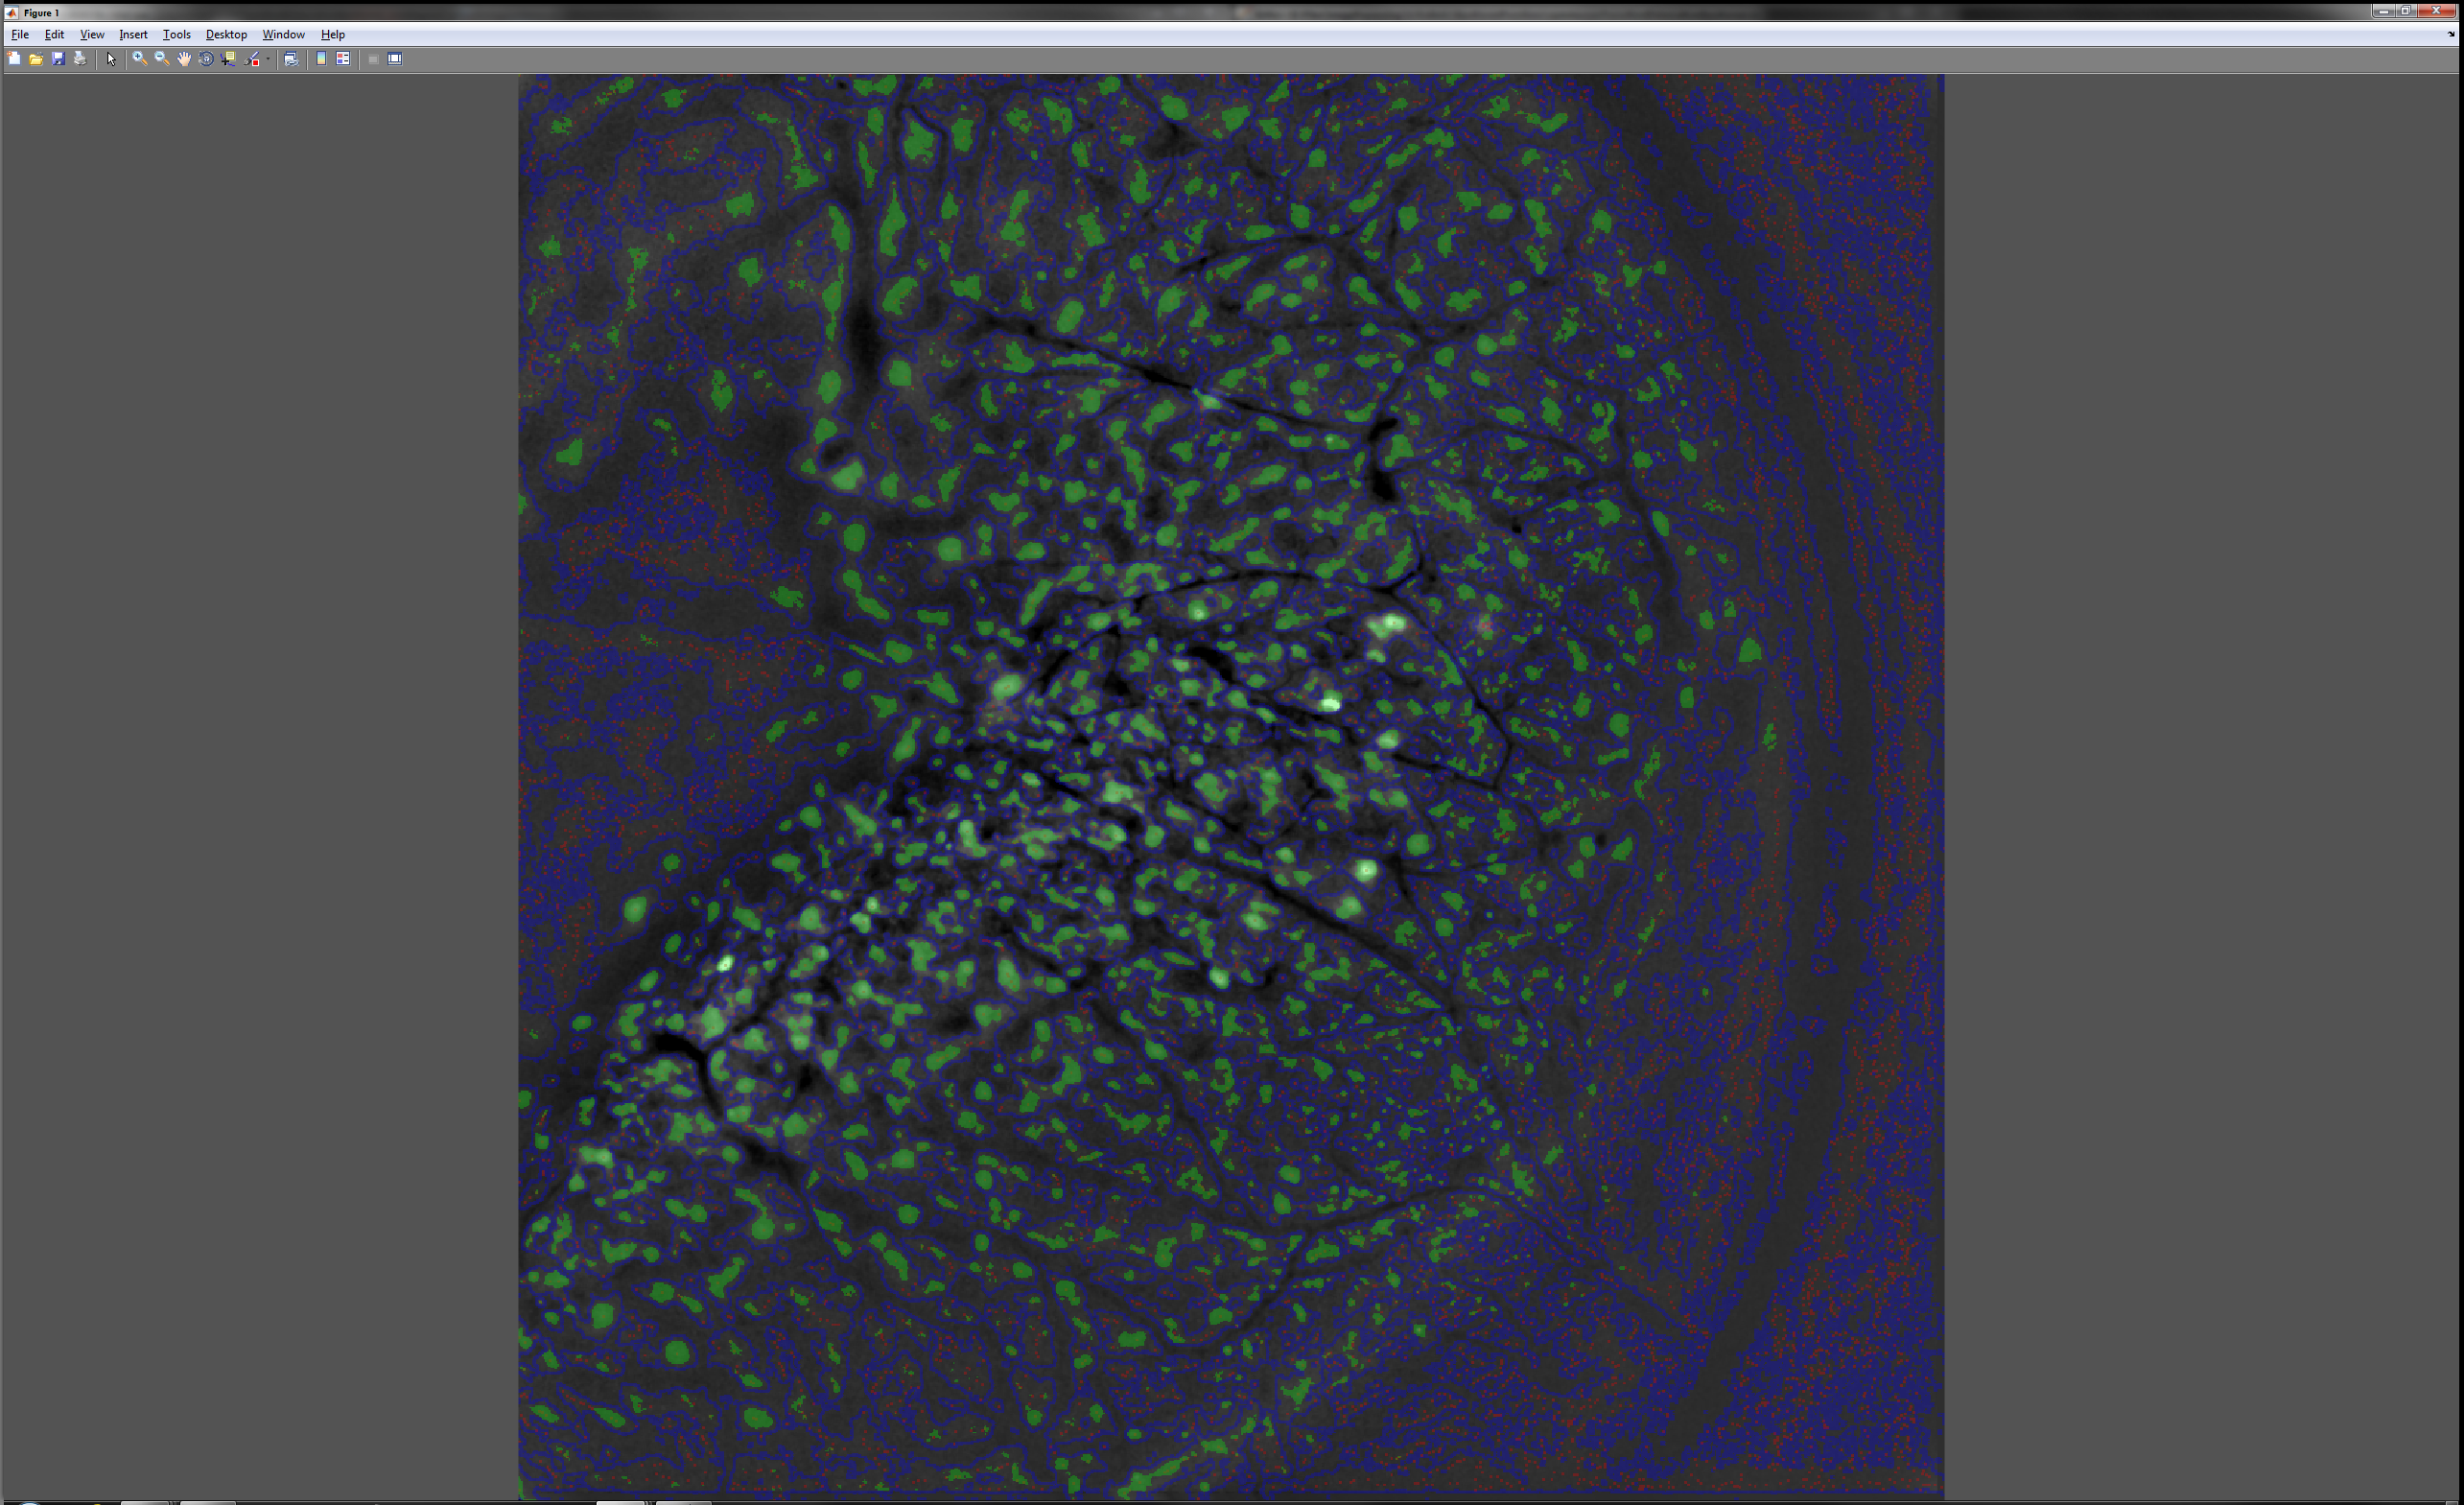
\includegraphics[height=12cm]{2.png}
% 	\caption{caption}
% \end{figure}

\begin{figure}[htb]\centering
	\includegraphics[height=12cm]{sw-video-processing-feature-pointwise-mutual-information.png}
	\caption{Feature generation of single motion-compensated frame using complex-valued normalized pointwise mutual information of each pixel with its local neghborhood}
\end{figure}


% \begin{figure}[htb]\centering
% 	\includegraphics[height=12cm]{trgb-013.png}
% 	\caption{caption}
% \end{figure}

\begin{figure}[htb]\centering
	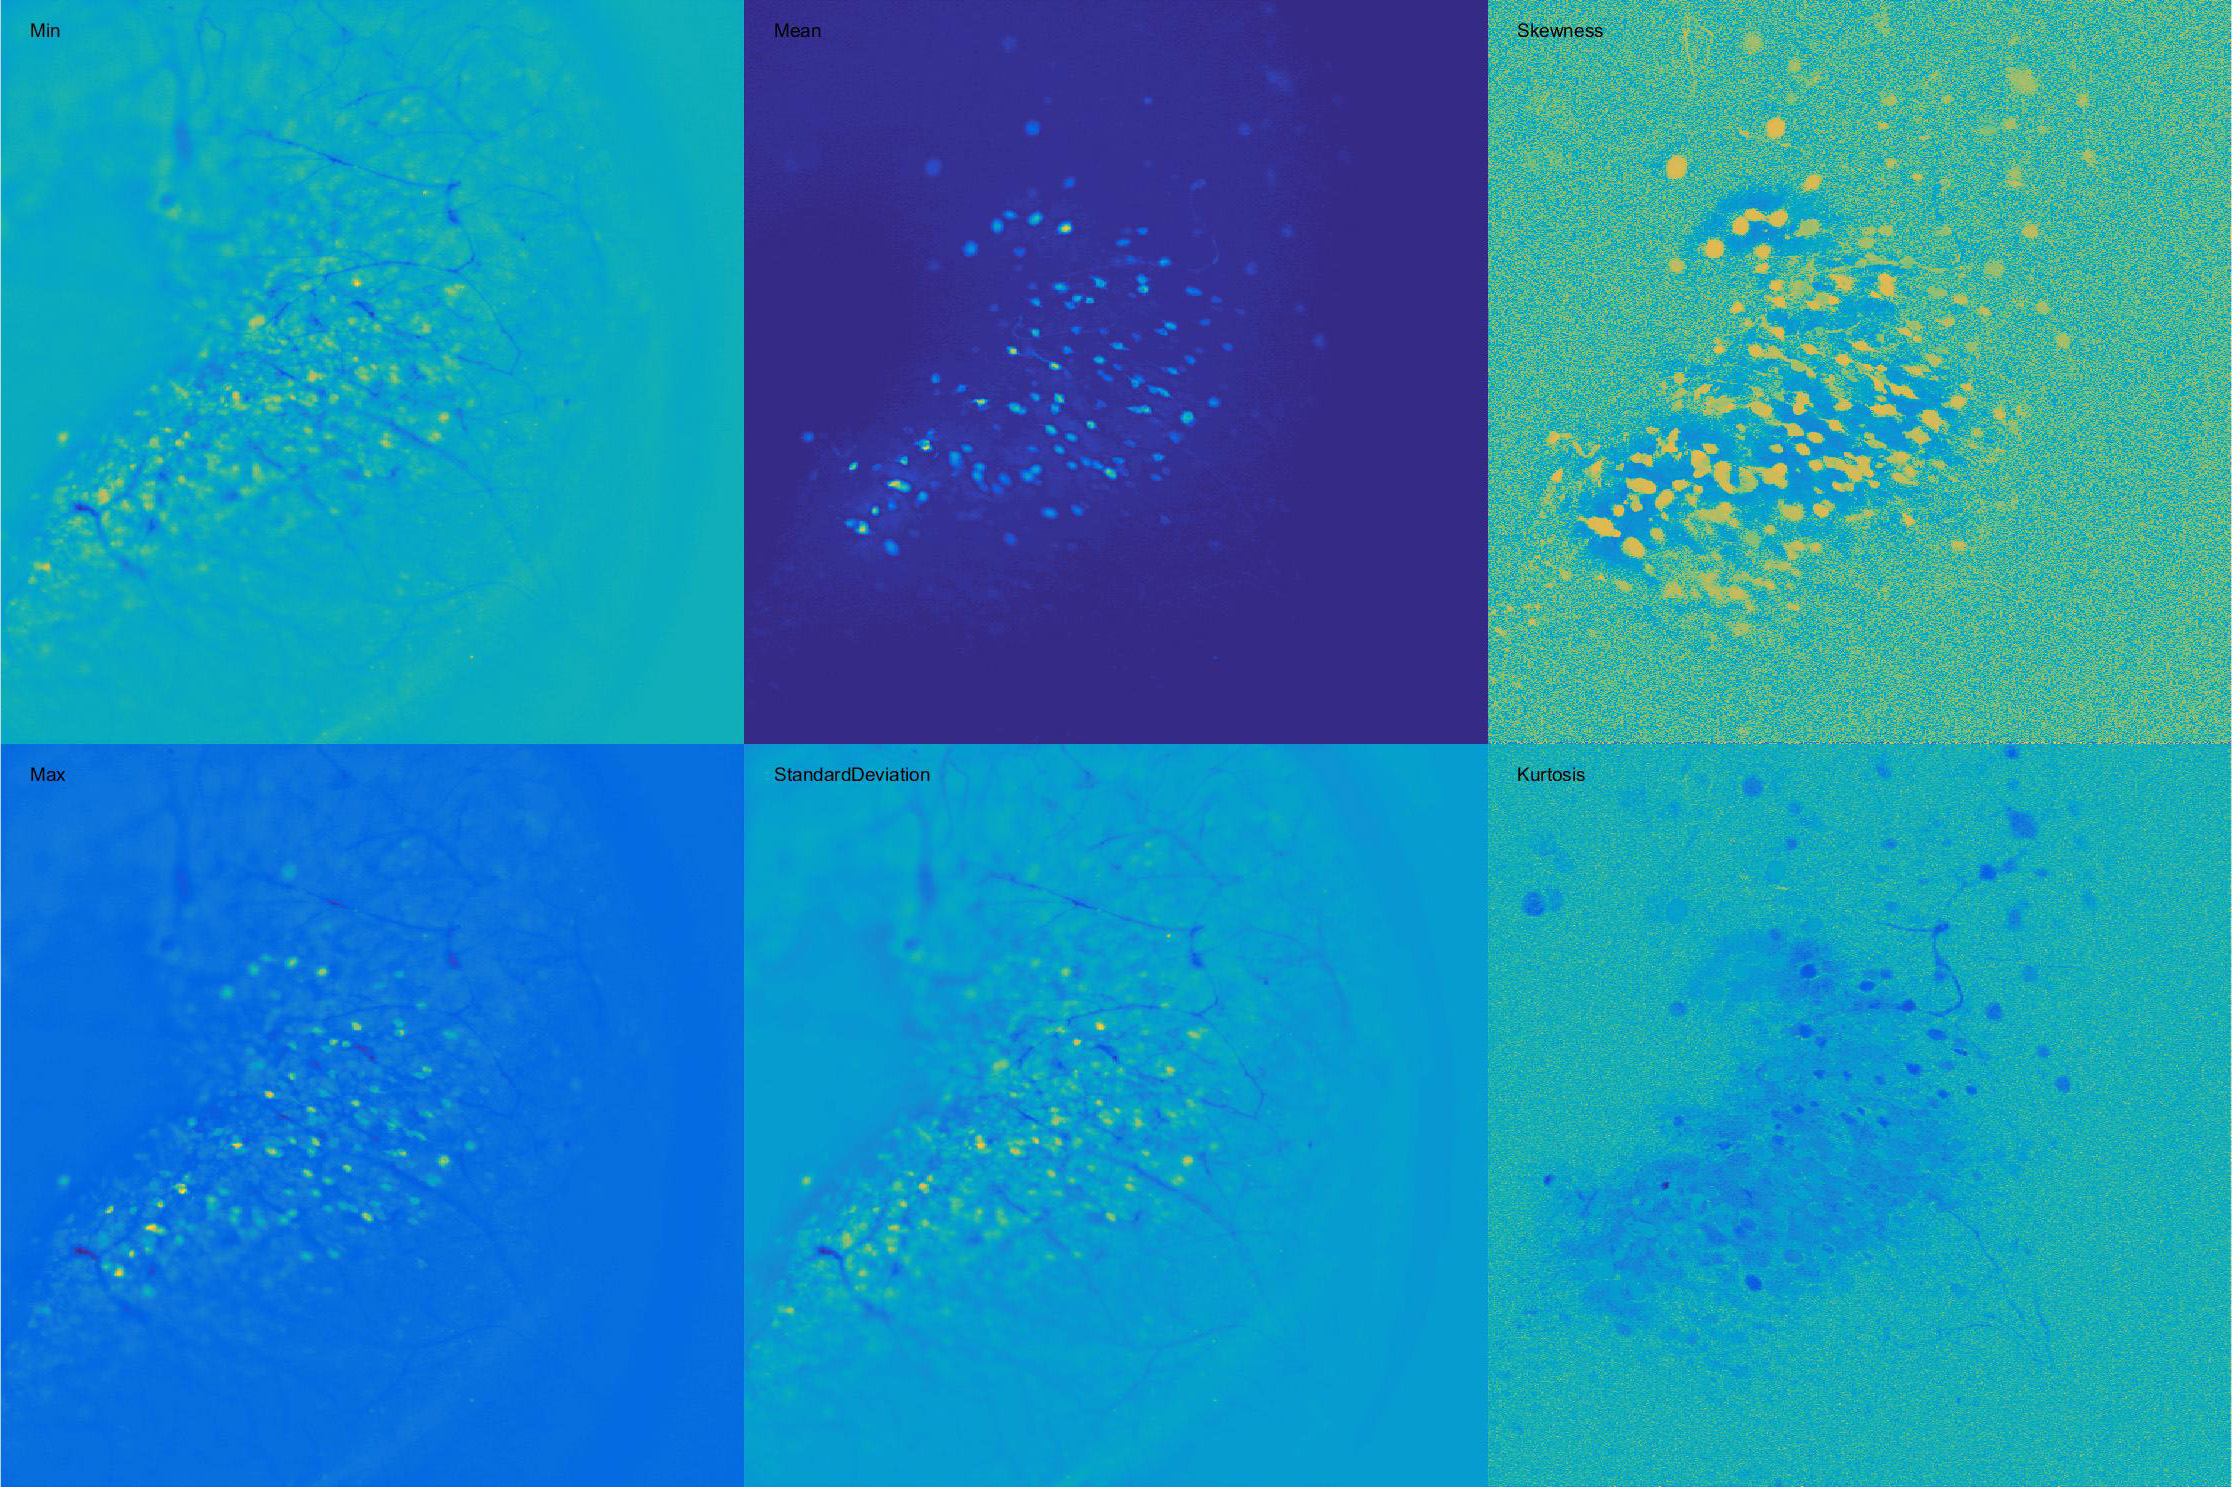
\includegraphics[width=12cm]{statistics_of_128_frames_contrast_enhanced.jpg}
	\caption{Pixel-wise statistics of 128 frames (min, max, mean, standard deviation, skewness, kurtosis)}
\end{figure}


\begin{figure}[htb]\centering
	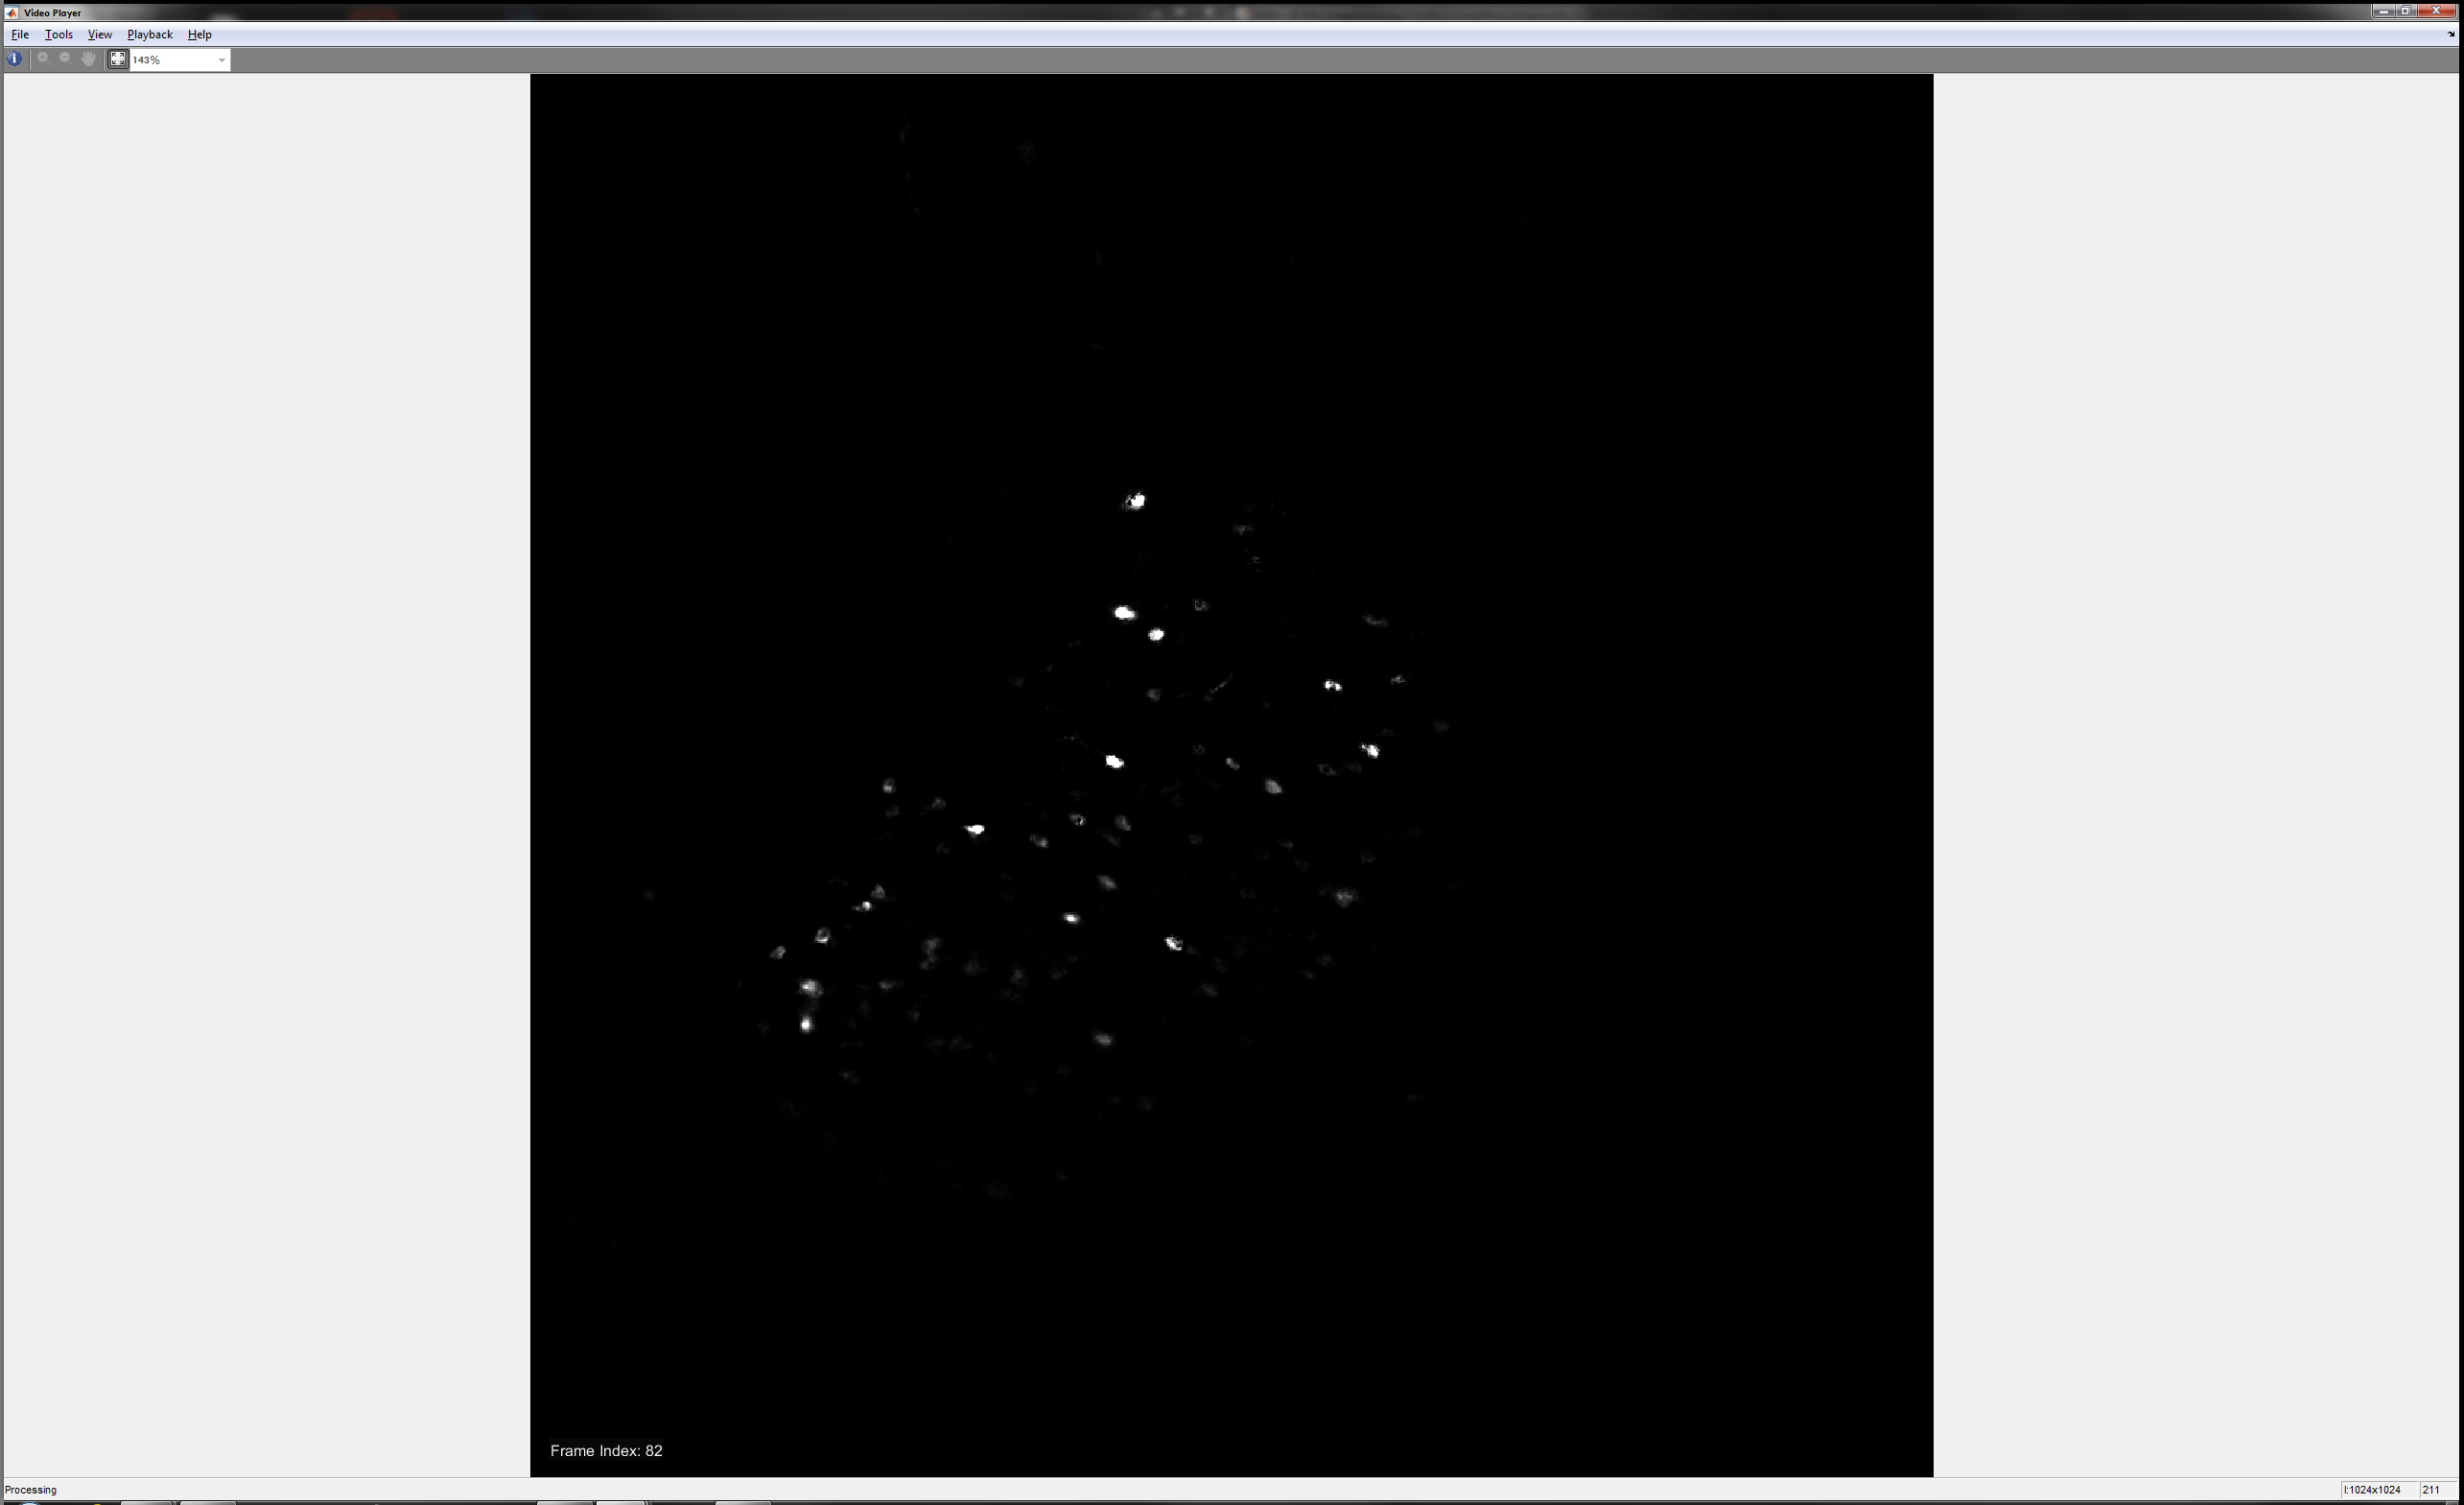
\includegraphics[width=12cm]{sw-sequence-bw.png}
	\caption{Normalized differential skewness}
\end{figure}

\clearpage


\end{document}

\cleardoublepage{}


% CHAPTER 4: DISCUSSION
\documentclass[../main.tex]{subfiles}
\begin{document}

\thispagestyle{myheadings}

\textbf{the last mile in computing for clinicians, engineers, and research scientists.
	..}

This dissertation presents straightforward and reproducible methods for assembling laboratory equipment that can capture the behavior and neural activity of laboratory animals as well as the procedures for managing and analyzing the collected data.
In some ways, the recommended procedures deviate from standard practice or the most obvious approaches.
In this section, the newer approaches are compared and contrasted with current or traditional ones.

\section{
  State of current methods}
\label{state-of-current-methods}

At the start of the work described here, we found ourselves with technology providing “neural signals” that vastly exceeded our expectations and the assumptions of the tools we applied to work with it.
In the past, fluctations in optical imaging data were dominated by “noise.
” The form of noise depended on the process; all types of imaging, intrinsic signal, fluorescent dye, etc., had relatively small fluctuations resulting from neural activity.
With new engineered molecules, like GCaMP6, and new images sensors, like those dubbed scientific CMOS, these sources of noise were comparatively small.
This improved signal-to-noise ratio opens the door for new opportunities and facilitates change to traditional analytic routines.
The abundance of signals available from our research animals not only makes old routines inefficient, but paradoxically, also insufficient.
Such an abundance of data factors at our finger tips requires a level of discipline in study design to make the scientific method work that was previously unnecessary as the difficulty in finding signals was inherently “self regulating” and inherently limiting.

\subsection{
	Signal and Noise in Neural Imaging Data}
\label{signal-and-noise-in-neural-imaging-data}

Traditional noise in neural signals can be roughly categorized as having origin in physiology or technology.
The physiological noise sources include “artifacts” caused by an animal’s breathing, heart beat, or other physical movements in response to the experimentally controlled world around them.
Technological noise is usually broken down into sensor noise sources:  read noise and thermal noise, and noise relating to digitization.
A third type of “noise” could arguably be categorized as either, as it lies at the interface of technology and biology.
For example, the complex interactions of exogenous calcium-binding proteins like GCaMP with the endogenous calcium handling proteins of a neuron potentially creates noise at the technology-biology interface.
By strict definition, however, only the sensor noise should termed noise, as other sources are mostly predictable and unpredictable and can be systematically neutralized or accommodated prior to data analysis.
The noise level in the signals gathered by a combination of GCaMP6 and a sCMOS camera is miniscule relative to the signals indicating fluctuation in calcium concentration.
The problem of visualization of these signals persists however, as the dynamic range of signal varies tremendously over space and time, and requires some treatment prior to being displayed on our currently limited computer monitors.
Previously common methods, particularly intrinsic-signal imaging, provided very small signals that required “averaging over time” before any specific or reproducible response could be ascertained.

\subsection{
	Correlation, Confounding Signals, and Non-linear dyanamics}
\label{correlation-confounding-signals-and-non-linear-dyanamics}

\subsection{Motion Artifact}
\label{motion-artifact}

\section{Exponential Expansion in Data Volume}
\label{exponential-expansion-in-data-volume}

The quality of cheaply available image sensors has risen drastically and are readily available.
A workable interface can be readily established and the stream of information they provide once switched on is virtually unlimited.
In the stark contrast however, storage for this never-ending data stream is both finite in its capacity, and cumulative in its consumption of available storage devices.

\subsection{
	Fields sharing these challenges}
\label{fields-sharing-this-challenges}

Scientists often view themselves as working inside laboratory full of sensors, being “data-rich” but “space-poor”.
For better or worse, scientists are not alone in dealing with this inherent technologic problem.
Massive investment has been poured into managing this issue for commercial purposes, and – perhaps unsettlingly – for governmental surveillance purposes.
The volume of recordable traffic bouncing through choke points of the internet exceeds the capacity of any government to store for more than about 24 hours.
Likewise, the massive volume of video data acquired by video surveillance systems in China requires a similar solution to one desired by scientists and physicians to resolve our data acquisition challenges.

\subsection{
	Technological Opportunities to Expect}
\label{technological-opportunities-to-expect}

Current solutions proposed by commercial and governmental giants are not radical.
They include calls for standardization in data format that could enable solutions for efficient transmission and storage to be shared by improving common tools.
Common streaming formats allow compression and storage to be abstracted from each application.
Databases are being developed to take advantage of heterogeneous computational architectures and distributed storage spaces.
Traditional document-based or relational databases are outperformed by graph-based “triple-store” databases, timeseries databases, and by databases programmed for specific architecture, including GPU-databases.
These technologic developments are targeted at the bottlenecks currently restricting access to data.
Early results with these approaches suggest an orders of magnitude improvement in throughput.
These tools are being developed both with and without the contribution of physicians and scientists.
It would be prudent however, to take advantage of new developments by orienting these tools to the specific needs of scientists and clinicians.

\section{
  Clinical translation potential}
\label{clinical-translation-potential}

Devices that rely on optogenetics to deliver stimulation to neurons inherently share the same hurdles to clinical translation.
These hurdles include the requirement for gene-therapy and its associated risks.
Several early trials of viral transfection of cells had adverse effects including a greatly increased risk of carcinoma.
In these early studies, the DNA insertion location was uncontrolled leaving important regions of DNA tumor suppressor genes exposed to damage.
New methods that improve the safety of gene therapy have been developed.
Several of the more recent methods utilize adeno-associated virus (AAV) with greater control regarding the site of DNA insertion and also cause less DNA damage.
These more recent methods suggest the possibility that with continuing research, methods may be developed without the inherent potential to stimulate malignancy.
Working on a project that requires a technology that does not as of yet exist represents one of the greatest educational challenges and benefits of this project.
That leap of faith into a future that also does not exist requires us to depend on each other as a team of collaborators in a mutually interdependent manner.
In order to succeed, we must do so together.
Without each other, our therapeutics would never reach their ultimate “target audience”, the patient.
In this scenario, we share both successes and setbacks in the same meaningful way whether such events occur within our own labs or others located elsewhere.

\section{
  Cranial Window}
\label{cranial-window}

The two-stage cranial implant device described here was developed to enable reliable, long-term optical access and intermittent physical access to mouse neocortex.
Our particular application required bilateral cortical windows compatible with wide-field imaging through a fluorescence microscope, and physical access to the underlying tissue for virus-mediated gene delivery and injection of exogenous labeled cells.
Optical access is required as soon as possible post-installation and ideally, is sustainable for several months thereafter.
My current designs are focused on addressing the issue common to other window designs meant for rodents, that is, progressive degradation of the optical light-path at the brain-to-window interface caused by highly scattering tissue growth.
The elastomer insert is molded to fit the chamber and craniotomy site, blocking tissue growth in way that provides a reliable optical interface lasting up to one year.
Additionally, the core design can be rapidly adapted to improve its performance or interface with diverse applications.

\subsection{“Biomimicry” in visual processing}
This section describes how computer image and video processing relate to visual processing in the mammalian brain.
The overall goal is to emphasize the advantage and importance of biomimetic development.
Neuromorphic computing with “on chip” image processing repsents an improvement over “edge computing”.
Event-based image sensors such as the “artificial retina”or tittto attempt to replicate physiologic environments  wherein event streams are demanded that are asynchronous and threshold-based.
Convolutional neural-nets and deep learning for specific tasks have secveal but also have substantial technlgoic similarities differences.
Genetic programming approaches to procedure optimization will hopefully minimize latency whle maximizing sensitivity and accuracy at minimal  computational cost, energy expenditure (i.e., with high metabolic efficiency) that facilitates visual stream processing amenable to feature extraction with motion estimation and compensation.
The current asymmetry of learning/training time negatively impacts on the  desired inference computation time.
Common standards applied across projects with common themes can be facilitatied by employing rigorous adherence to non-proprietary open source conventions that includes (bt is not limited to) optical parts (lens threads), file formats, widely available software libraries in standard programming languages, and ease of file transmission that are web-based.
We are well advised to borrow from related sectors with better developed solutions such as surveillance, media streaming for web/entertainment, sports, astronomy/telescopes, medical imaging and even automotive applications.

\subsection{
	Critical Elements}
\label{critical-elements}

In assessing the design presented here, we highlight a few critical elements that facilitate the maintenance of the long-term optical quality.
The Methods section describes the specifics of surgical procedures for headplate installation and insert attachment.
These procedures were established after testing the variable formulations in protocol.
First, the design of the silicone insert must incorporate a mechanical barrier that fits along the edges of the craniotomy.
To be effective, the barrier must be continuous along the circumference, and extend as far as the inside surface of the skull.
Achieving this tight fit without agressively impinging on the brain requires some sort of fine height adjustment capability.
The silicone insert must be attached at the correct height during the installation procedure, or shortly thereafter.
The insert must be slightly depressed until full contact is made across the entire window.
However, pressing beyond this distance quickly exerts an untoward increase in intracranial pressure that promotes both inflammation and adverse outcomes.
A mechanism for fine adjustment can be designed into the system and is in fact incorporated into the installation procedure as is done in the first design and demonstrated in the second design presented here.
Of particular note, we found that administration of antibiotic and anti-inflammatory drugs in the days surrounding any major surgical procedure had a substantial impact on the viability of the optical interface.
We used both corticosteroid and non-steroidal anti-inflammatory drugs.
Attempts to exclude either drug caused poor outcomes for study animals.
Lastly, sealing the chamber is absolutely critical for achieving viability of the optical interface as well as the animal’s overall well being.
Equally critical to the long-term health of the imaging chamber is the requirement to establish and maintain an air-tight seal between the chamber and the outside world.
This includes a permanent seal between the chamber and skull and a reversible seal between the chamber rim and the optical insert.
is Although specific to the system design, a permanent seal is absolutely essential to ensure long-term functionality.
In addition to establishing and maintaining an air-tight seal, it is necessary to eliminate all air pockets within the chamber.
Residual air pockets will be susceptible to bacteria growth and may disrupt normal intracranial and intermembrane pressures after installation.
We employed sterile agarose fill to displace all air within the chamber prior to sealing.
Dead space surrounding the silicone insert, including that temporarily filled with agarose, will fill with fluid and eventually be overtaken by granulation tissue.
This preventive process is helpful to the maintenance of a sterile chamber environment and therefore, care should be taken not to disrupt it.
However, an excess of dead space will delay this process and thus should also be minimized when adapting the design.
Several attempts to test variations from the described procedures indicated that all elements mentioned above are equally critical to achieving a reliable imaging window with sustained optical quality.
Implementing the procedures as described or an effective alternative solution should mitigate the primary obstacle to long-term imaging in mice and other rodents by reducing the need to pre-terminate imaging experiments due to light-path disruption by tissue ingrowth.
This capability will drastically reduce wasted time and resources for experiments of any duration and facilitate previously infeasible research that require longer-term observations including aging or progressive chronic neurological disorders.

\subsection{
	Staging Implant Installation \& Tissue Access}
\label{staging-implant-installation-tissue-access}

Configuring the implant as described to enable a staged installation of multiple parts enables surgical procedures to be easily spread across multiple days.
This capability offers a number of advantages including saving time and resources, particularly during the prototype stages by allowing time to ensure each implanted animal fully recovers from the initial procedure and anesthesia.
Additionally, the delay between surgeries allows the initial inflammation and immune system responses triggered by craniotomy to resolve before attempting a second intervention in tissue that is sensitive to these manipulations (e.g., viral or cell injections).
Importantly, this system affords the capability to image the first tissue intervention from day 0.
Similarly, designing a system installed in multiple stages enables trivial and repeatable tissue access at later time points by simply reversing the insert attachment procedure.
The process may be comparable to a previously reported method of removing the entire cranial glass window to access the tissue.
With this newer system however, the methods used to detach and reattach the cranial window are relatively faster, simpler and carry less risk of tissue damage.
Additionallly, the described methodd provide full cranial access without compromising the image field, an advantage not provided by a fixed access port.

\subsection{
	Design Adaptation}
\label{design-adaptation}

The specific designs described in this report work well and have much to offer.
The potential for fast and unrestricted adaptation is the greatest asset of the underlying system.
Most users will find greater utility in adopting components of the design and fabrication process that can be readily customized to fit their exact needs.
The design can also be rapidly transformed to accommodate various applications or to modify its performance in response to new technologies and demands.
This rapid adaptability was a primary goal of this projec, and informed our design and engineering decisions throughout developement.
Anyone with access to common laboratory equipment and moderate engineering and fabrication skills can produce a system to fit their particular needs.
As an inherent aspect of any design process, the adaptation of the original design evolved over the course of prototyping and testing.
In presenting two designs in this report, our intention was to demonstrate the technical feasibility of continuous development of a “future-proof” system.
The original system was adapted to accomodate the continuous evolution of image sensor technology, particularly the growth in size and resolution, expanding the field of view and allowing simultaneous access to cellular interactions across multiple brain regions using wide-field imaging.
We found that subtle dimensional changes, and the addition of miniscule features exert a large impact on the success of any design.
We also found that adjusting features to address one aspect of functionality may have unintended effects.
For example, the inclusion of a thin skirt extending below the optical insert that was incorporated to protect against tissue growth within the image field also promotes physical conformity of the brain to the optical window interface over time.
This conformity results in a flat imaging plane that is optimal for wide-field imaging and was previously unachievable.

\subsection{
	Rapid fabrication}
\label{rapid-fabrication}
The rapid iterative process used here was made possible by using a combination of widely available rapid prototyping procedures, 3D-printing and laser-cutting.
Major progress of manufacturing and its increased versatility, providing better quality, customization, lower cost and shorter production time.
In an effort to compare various manufacturing technologies, we explored a number of companies and advanced with 3D metal printing.
The final products provided by at i.materialise achieved our experimental goals in product design.
We also developed parts in collaboration with other rapid prototyping companies including Shapeways and Sculpteo.
In addition:
\begin{itemize}
	\item	Various features and functions of the silicone insert were transformed and extended to conform to new design requirements, some requiring distinctively different design approaches
	\item	Versatility of silicone elastomer to cover a spectrum of design strategies to optimize its configuration might be beneficial
	\item	The design principles that evolved from the initial development are robust and can be applied to new developments or refinements while preserving the successful qualities of the original implant
	\item	CAD designs of these reported systems are open source accessible and can be modified and extended by evolving demands and technologies We, the authors, also call for replication, adaptation, and evaluation (i.e., continued open/shared development).
\end{itemize}
\subsection{
	Future improvements} The current project primarily explores the ability to mold precise and complex features using silicone elastomer to discover configurations to improve image performance using encapsulated electrodes and optical guides.
These approaches replace combination optical + integrated electrode window and do not require optogenetics stimulation.
More significantly, the encapsulation of carbon, metal colloidal particles or quantum dots into polymer hydrogel networks imparts exclusive thermal, sonic, optical, electrical or magnetic properties.
Specifically, the polymer interface may provides a means for directly penetrating neurons to gain electrophysiological recording or facilitate drug infusions, allowing recording and/or manipulation during imaging session.
In the near future, improvments in window thickness and chromatic aberration wil enhance both wider-field and 2-photon imaging, aprocess that will be enhanced by improved and lenses and embeded, integrated electronic components, such as LEDs for illumination or stimulation, or sensors.
These mbedded devices will facilitate positioning, especially in combination with kinematic headplates that alow for repeatable head positioning and newer fabrication materials.

\clearpage

\end{document}



%%%%%%%%%%%%%%%%%%%%%%%%%%%%%%%%%%%%%%%%%%%%%%%%%%%%%%%%%%%%%%%%
% POST (everything following main text)
%%%%%%%%%%%%%%%%%%%%%%%%%%%%%%%%%%%%%%%%%%%%%%%%%%%%%%%%%%%%%%%%

% APPENDIX
\begin{appendices}
  % \chapter{Appendix}
% \label{appendix1}

\chapter{Published Abstracts}
\label{sec:published-abstracts}
\thispagestyle{myheadings}
\section*{An integrative approach for analyzing hundreds of neurons in task performing mice using wide-field calcium imaging}
\label{sec:ali}

Advances in neurotechnology have been integral to the investigation of neural circuit function in systems neuroscience.
Recent improvements in high performance fluorescent sensors and scientific CMOS cameras enables optical imaging of neural networks at a much larger scale.
While exciting technical advances demonstrate the potential of this technique, further improvement in data acquisition and analysis, especially those that allow effective processing of increasingly larger datasets, would greatly promote the application of optical imaging in systems neuroscience.
Here we demonstrate the ability of wide-field imaging to capture the concurrent dynamic activity from hundreds to thousands of neurons over millimeters of brain tissue in behaving mice.
This system allows the visualization of morphological details at a higher spatial resolution than has been previously achieved using similar functional imaging modalities.
To analyze the expansive data sets, we developed software to facilitate rapid downstream data processing.
Using this system, we show that a large fraction of anatomically distinct hippocampal neurons respond to discrete environmental stimuli associated with classical conditioning, and that the observed temporal dynamics of transient calcium signals are sufficient for exploring certain spatiotemporal features of large neural networks.

\noindent
Published 2016 \cite{Mohammed_2016}
\clearpage


\section*{Striatal cholinergic interneurons generate beta and gamma oscillations in the corticostriatal circuit and produce motor deficits}
\label{sec:kk}

Cortico-basal ganglia-thalamic (CBT) neural circuits are critical modulators of cognitive and motor function.
When compromised, these circuits contribute to neurological and psychiatric disorders, such as Parkinson’s disease (PD).
In PD, motor deficits correlate with the emergence of exaggerated beta frequency (15–30 Hz) oscillations throughout the CBT network.
However, little is known about how specific cell types within individual CBT brain regions support the generation, propagation, and interaction of oscillatory dynamics throughout the CBT circuit or how specific oscillatory dynamics are related to motor function.
Here, we investigated the role of striatal cholinergic interneurons (SChIs) in generating beta and gamma oscillations in cortical-striatal circuits and in influencing movement behavior.
We found that selective stimulation of SChIs via optogenetics in normal mice robustly and reversibly amplified beta and gamma oscillations that are supported by distinct mechanisms within striatal-cortical circuits.
Whereas beta oscillations are supported robustly in the striatum and all layers of primary motor cortex (M1) through a muscarinic-receptor mediated mechanism, gamma oscillations are largely restricted to the striatum and the deeper layers of M1.
Finally, SChI activation led to parkinsonian-like motor deficits in otherwise normal mice.
These results highlight the important role of striatal cholinergic interneurons in supporting oscillations in the CBT network that are closely related to movement and parkinsonian motor symptoms.

\noindent
Published 2016 \cite{Kondabolu_2016}

\clearpage


\section*{Young adult born neurons enhance hippocampal dependent performance via influences on bilateral networks}
\label{sec:jm}

Adult neurogenesis supports performance in many hippocampal dependent tasks.
Considering the small number of adult-born neurons generated at any given time, it is surprising that this sparse population of cells can substantially influence behavior.
Recent studies have demonstrated that heightened excitability and plasticity may be critical for the contribution of young adult-born cells for certain tasks.
What is not well understood is how these unique biophysical and synaptic properties may translate to networks that support behavioral function.
Here we employed a location discrimination task in mice while using optogenetics to transiently silence adult-born neurons at different ages.
We discovered that adult-born neurons promote location discrimination during early stages of development but only if they undergo maturation during task acquisition.
Silencing of young adult-born neurons also produced changes extending to the contralateral hippocampus, detectable by both electrophysiology and fMRI measurements, suggesting young neurons may modulate location discrimination through influences on bilateral hippocampal networks.

\noindent
Published 2016 \cite{Zhuo_2016}
\clearpage


\section*{A Teensy microcontroller-based interface for optical imaging camera control during behavioral experiments}
\label{sec:mr}

\subsubsection*{Background}
Systems neuroscience experiments often require the integration of precisely timed data acquisition and behavioral monitoring.
While specialized commercial systems have been designed to meet various needs of data acquisition and device control, they often fail to offer flexibility to interface with new instruments and variable behavioral experimental designs.

\subsubsection*{New method}
We developed a Teensy 3.2 microcontroller-based interface that is easily programmable, and offers high-speed, precisely timed behavioral data acquisition and digital and analog outputs for controlling sCMOS cameras and other devices.

\subsubsection*{Results}
We demonstrate the flexibility and the temporal precision of the Teensy interface in two experimental settings. In one example, we used the Teensy interface to record an animal’s directional movement on a spherical treadmill, while delivering repeated digital pulses that can be used to control image acquisition from a sCMOS camera.
In another example, we used the Teensy interface to deliver an auditory stimulus and a gentle eye puff at precise times in a trace conditioning eye blink behavioral paradigm, while delivering repeated digital pulses to trigger camera image acquisition.

\subsubsection*{Comparison with existing methods}
This interface allows high-speed and temporally precise digital data acquisition and device control during diverse behavioral experiments.

\subsubsection*{Conclusion}
The Teensy interface, consisting of a Teensy 3.2 and custom software functions, provides a temporally precise, low-cost, and flexible platform to integrate sCMOS camera control into behavioral experiments.

\noindent
Published 2019 \cite{Romano_2019}


\clearpage


\section*{Unique contributions of parvalbumin and cholinergic interneurons in organizing striatal networks during movement}
\label{sec:hg}

Striatal parvalbumin (PV) and cholinergic interneurons (CHIs) are poised to play major roles in behavior by coordinating the networks of medium spiny cells that relay motor output.
However, the small numbers and scattered distribution of these cells have hindered direct assessment of their contribution to activity in networks of medium spiny neurons (MSNs) during behavior.
Here, we build on recent improvements in single-cell calcium imaging combined with optogenetics to test the capacity of PVs and CHIs to affect MSN activity and behavior in mice engaged in voluntary locomotion.
We find that PVs and CHIs have unique effects on MSN activity and dissociable roles in supporting movement.
PV cells facilitate movement by refining the activation of MSN networks responsible for movement execution.
CHIs, in contrast, synchronize activity within MSN networks to signal the end of a movement bout.
These results provide new insights into the striatal network activity that supports movement.

\noindent
Published 2019 \cite{Gritton_2019}
\clearpage



% \section{Project contribution 1 (2016)}
% 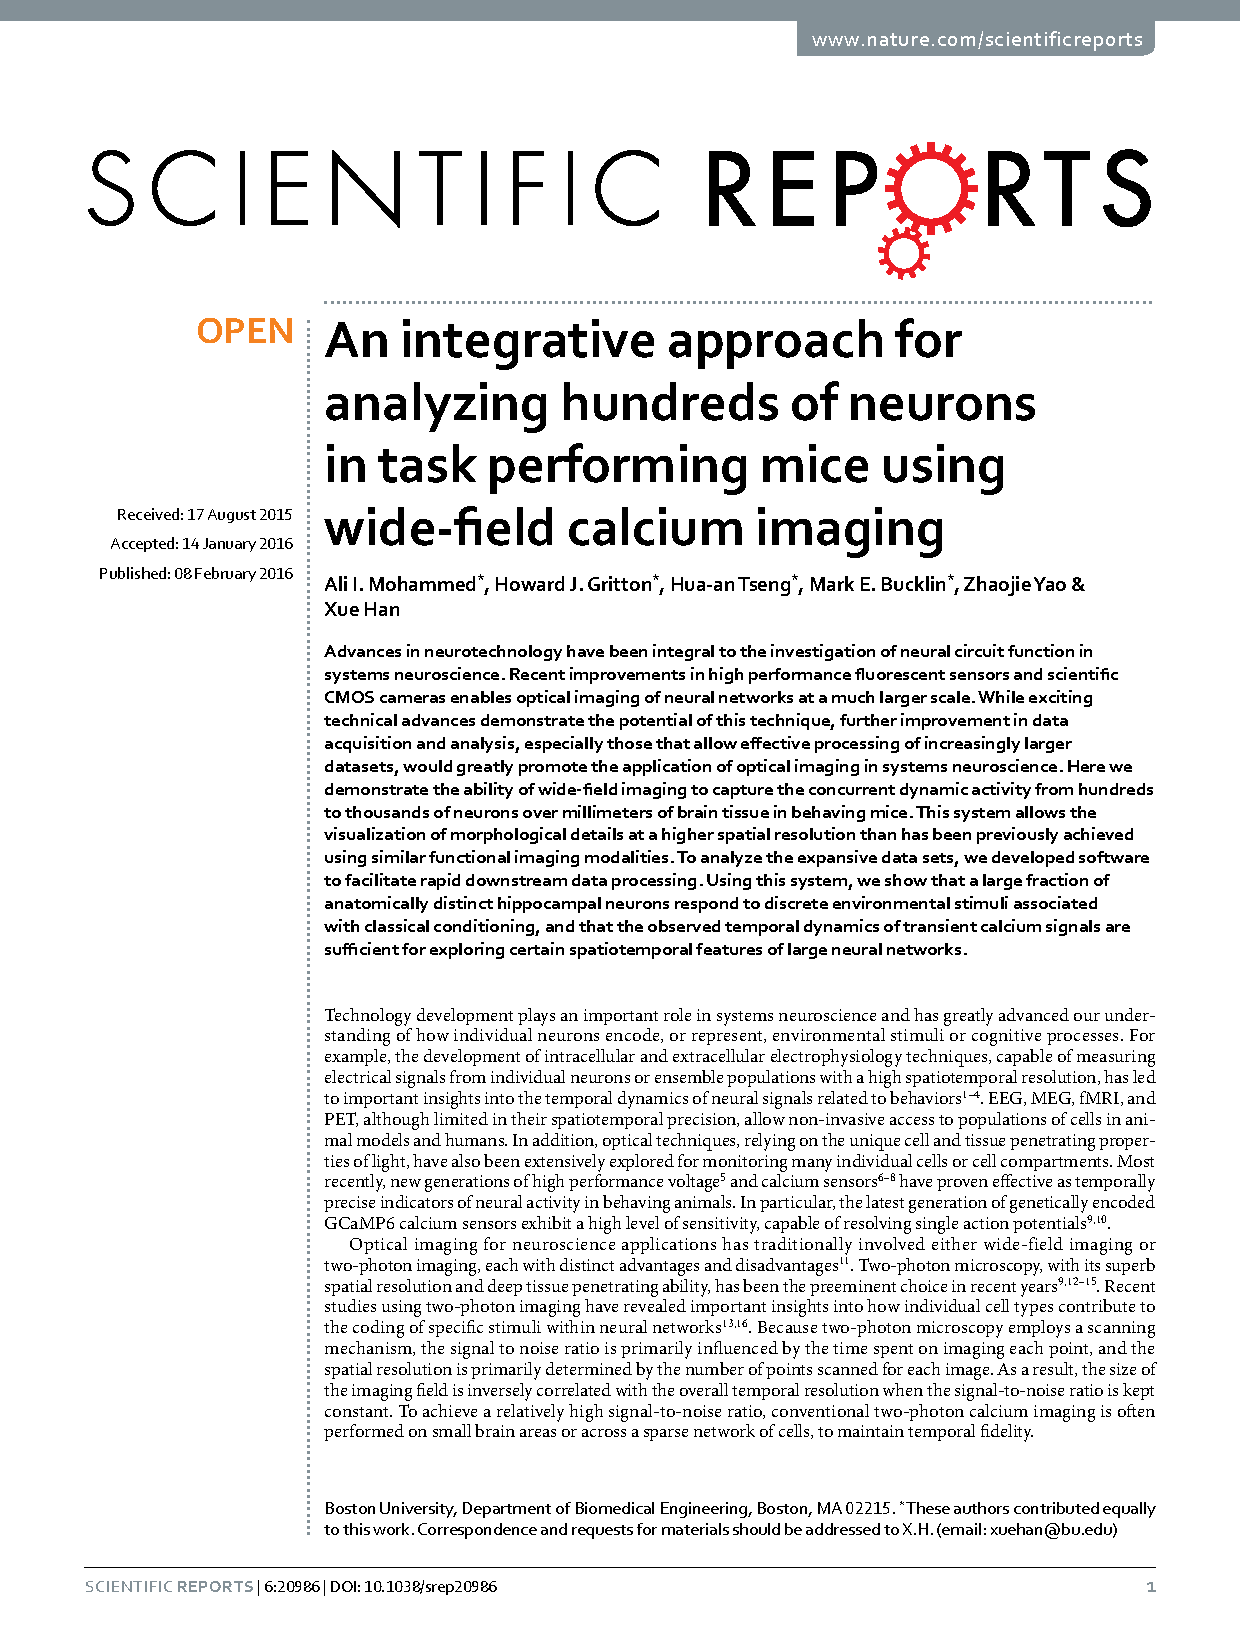
\includepdf[pages=-,templatesize={120mm}{175mm},scale=0.85]{appendix/ali.pdf}
% \section{Project contribution 2 (2016)}
% 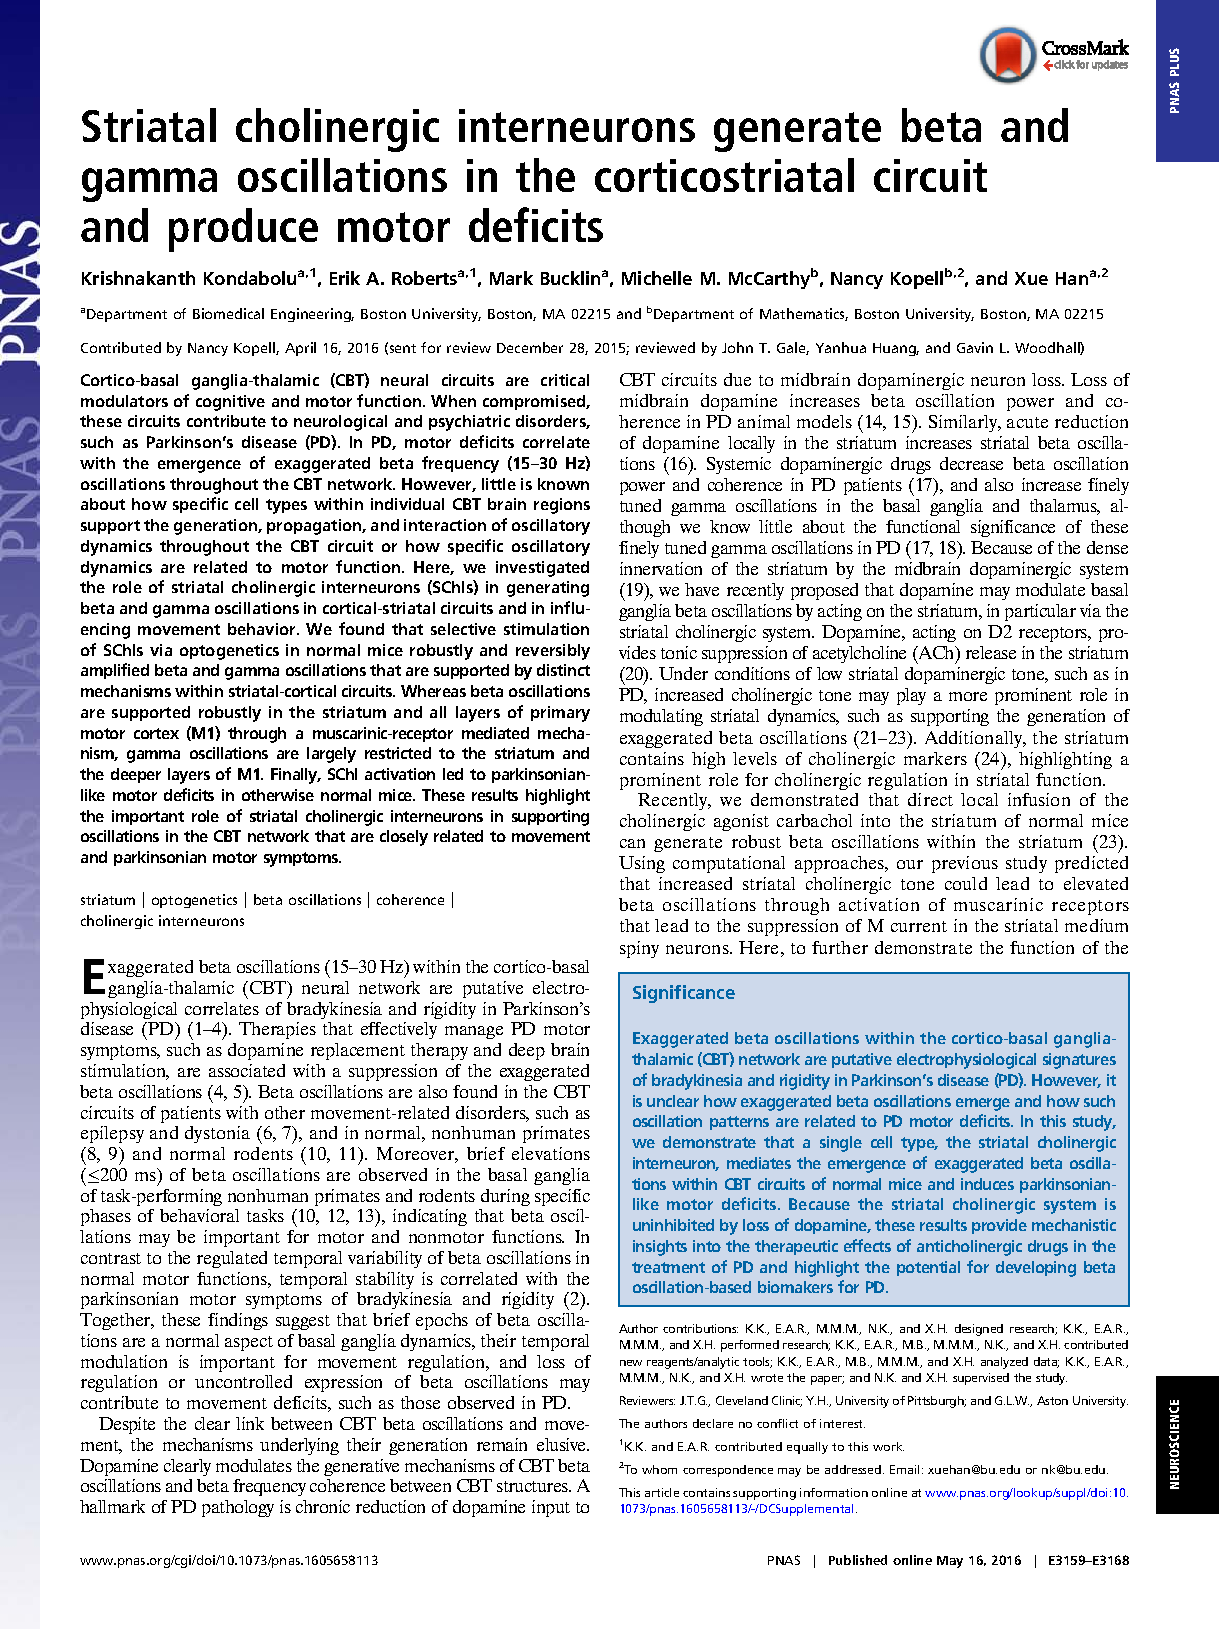
\includepdf[pages=-,templatesize={120mm}{175mm},scale=0.85]{appendix/kk.pdf}
% \section{Project contribution 3 (2016)}
% 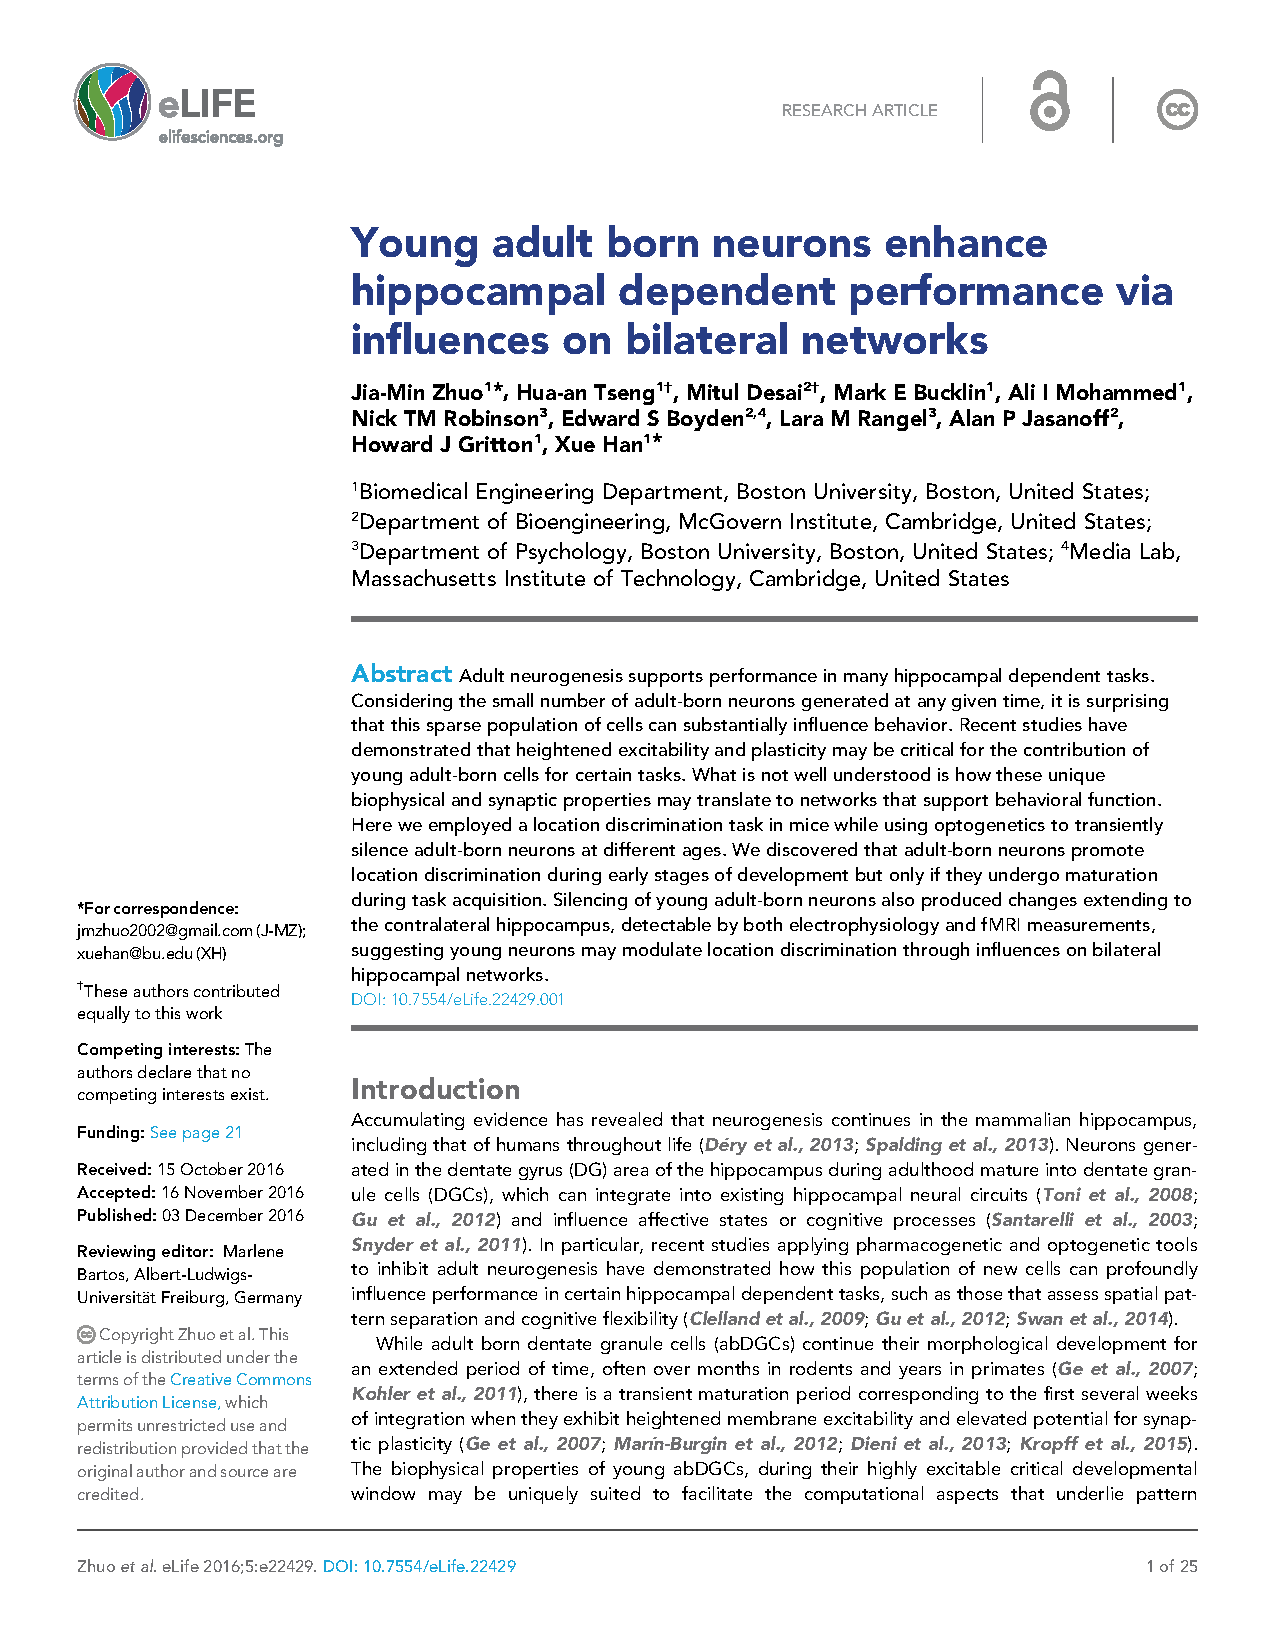
\includepdf[pages=-,templatesize={120mm}{175mm},scale=0.85]{appendix/jm.pdf}
% \section{Project contribution 4 (2019)}
% 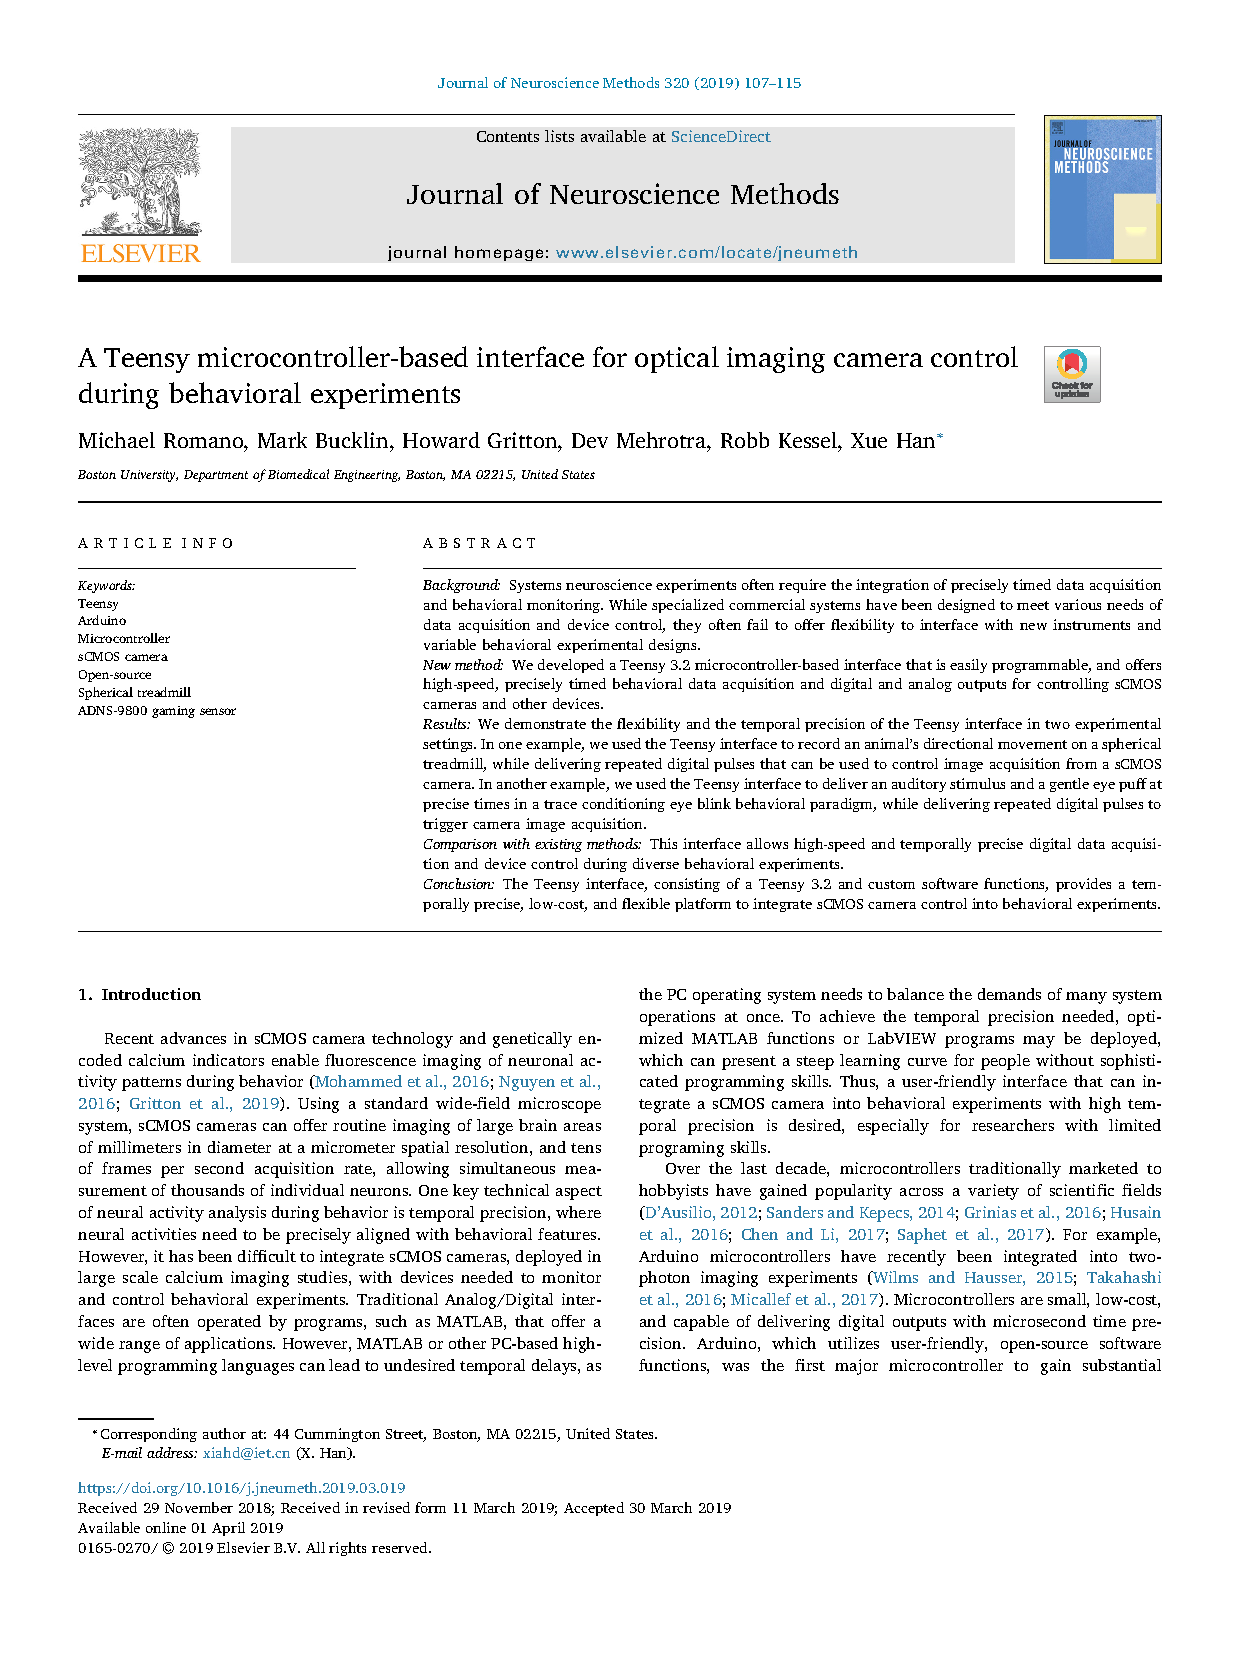
\includepdf[pages=-,templatesize={120mm}{175mm},scale=0.85]{appendix/mr.pdf}
% \section{Project contribution 5 (2019)}
% \includepdf[pages={1-17},templatesize={120mm}{175mm},scale=.85]{appendix/hg.pdf}

\end{appendices}

% BIBLIOGRAPHY
\nocite{*}
\clearpage
\phantomsection
\singlespace{}
\raggedright{}
% \renewcommand{\refname}{\section{Bibliography}} % Using "Sources" as the title of the section
% \addcontentsline{toc}{chapter}{Bibliography}
% \addcontentsline{toc}{chapter}{References}
% \printbibliography{thesis}
\thispagestyle{myheadings}
\bibliographystyle{apalike}
\bibliography{thesis}
% \thebibliography{thesis}
\clearpage{}

% CURRICULUM-VITA
\chapter*{Curriculum Vitae}\label{sec:cv}
\addcontentsline{toc}{chapter}{Curriculum Vitae}

\thispagestyle{empty}

\begin{center}
% {\LARGE {\bf CURRICULUM VITAE}}\\
% \vspace{0.5in}
{\large {\bf Mark E. Bucklin}}
\end{center}

6 Front St
Chelsea, MA 02150
markbucklin@gmail.com

\textbf{Education}

\begin{quote}
\textbf{BOSTON UNIVERSITY,}

\textbf{School of Medicine; Division of Graduate Medical Sciences}

\textbf{Boston, MA}

\emph{2010-Present}
\end{quote}

\begin{itemize}
\item
  Currently in 1\textsuperscript{st} year of M.D./Ph.D.~program
\item
  Pursuing Ph.D.~in Biomedical Engineering
\end{itemize}

\begin{quote}
\textbf{COLUMBIA UNIVERSITY,}

\textbf{Fu Foundation School of Engineering and Applied Science}

\textbf{New York, NY}

\emph{2005-2009}
\end{quote}

\begin{itemize}
\item
  B.S. Biomedical Engineering -- Biomedical Imaging track
\item
  3.69 Cumulative GPA
\item
\end{itemize}

\begin{quote}
\textbf{MOUNT DESERT ISLAND HIGH SCHOOL}

\textbf{Bar Harbor, ME}
\end{quote}

\emph{2001-2005}

\textbf{Experience}

CENTER FOR NEUROBIOLOGY AND BEHAVIOR - CUMC

Technician: Lab of Aniruddha Das, Ph.D.

New York, NY

\begin{quote}
May 2008-August 2010
\end{quote}

\begin{itemize}
\item
  Developed image acquisition software in MATLAB and firmware in
  embedded C
\item
  Built routines for data management, analysis, visualization, and
  access over a network
\item
  Constructed a device to measure respiratory patterns in non-human
  primates
\item
  Upgraded optical imaging system to use optical fibers, enabling
  simultaneous dual-wavelength intrinsic signal imaging and
  neural-recording
\end{itemize}

NORTHEAST HARBOR AMBULANCE SERVICE

EMT/Ambulance Attendant

Northeast Harbor, ME

2005-Present

\begin{itemize}
\item
  Lead care or assist a paramedic
\item
  Completed Intermediate level course for higher level license
\item
  Started IVs, collected blood, and obtained ECGs during \textgreater100
  hours of clinical rotations
\end{itemize}

TEACHING AND PROJECTS ABROAD

Medical Volunteer

Nagoda Hospital, Sri Lanka

May-June 2006

\begin{itemize}
\item
  Assisted and observed local medical personnel in rounds and various
  procedures
\item
  Spent time in General, OB-GYN, Pediatric, Surgical, and Post-Mortem
  wards
\end{itemize}

JACKSON LABORATORY

Research Intern

Bar Harbor, ME

2003-2005

\begin{itemize}
\item
  Designed and led study determining the effect of a global growth
  hormone deficiency on atherosclerosis in mice
\item
  Bred and genotyped mice and performed histology to quantify arterial
  damage
\item
  Used PCR genotyping to identify QTLs, and taught procedures to
  incoming students
\end{itemize}

HANCOCK COUNTY MEDICAL MISSION

Surgeon's Assistant

Ibarra, Ecuador

March 2005

\begin{itemize}
\item
  Directly assisted one general and one vascular surgeon in more than 50
  operations
\item
  Provided free-healthcare while gaining valuable medical experience
\end{itemize}

\textbf{Skills and Interests}

\begin{quote}
PROGRAMMING: MATLAB, Java, C/C++

INTERESTS: Electronics, Sailing, Traveling, Web Development
\end{quote}

\textbf{References}

\begin{quote}
Aniruddha Das Ph.D., Center for Neurobiology and Behavior, CUMC --
\href{mailto:ad2069@columbia.edu}{\nolinkurl{ad2069@columbia.edu}}

Michael Dennis M.D., St.~Mary's Episcopal Church --
\href{mailto:newrinkle@aol.com}{\nolinkurl{newrinkle@aol.com}}

Heather Frazer, Pd.D., --
\href{mailto:Frazer@fau.edu}{\nolinkurl{Frazer@fau.edu}}
\end{quote}

\clearpage{}

\end{document}
